\documentclass[UTF8]{ctexart}
\usepackage{algorithm}
\usepackage{algorithmic}
\usepackage{subfigure}
\usepackage{amsmath,bm}
\usepackage{fancybox}
\usepackage{listings}
\usepackage{xcolor}
\usepackage{diagbox}
\usepackage{amssymb}
\usepackage{amsmath}
\usepackage{amsthm}
\usepackage{empheq}
\usepackage[framemethod=tikz]{mdframed}
\usepackage{mathtools}
\usepackage{fancyhdr} 
\usepackage{longtable,booktabs}                               
\usepackage{lastpage}                                           
\usepackage{layout} 


% 图表
\usepackage{array,multirow}
  \setlength\extrarowheight{2pt} % 行高增加
\usepackage{longtable}
\usepackage{graphicx}

\usepackage{listings}

\usepackage{xcolor}

	\definecolor{ocre}{RGB}{243,102,25}
	\definecolor{mygray}{RGB}{243,243,244}


\lstset{
columns=flexible,
numbers=left,
numberstyle=\footnotesize\color{darkgray}, 
basicstyle=\small\ttfamily,
stringstyle=\color{purple},
keywordstyle=\color[RGB]{40,40,255}\bfseries,
commentstyle=\it\color[RGB]{0,96,96},  
stringstyle=\rmfamily\slshape\color[RGB]{128,0,0}, 
showstringspaces=false,      
% directivestyle=\color{blue},
frame=shadowbox,
%framerule=0pt,
backgroundcolor=\color[RGB]{245,245,244},
escapeinside=``, %逃逸字符(1左面的键),用于显示中文
breaklines,
extendedchars=false,
%解决代码跨页时,章节标题,页眉等汉字不显示的问题
xleftmargin=2em,xrightmargin=2em,
aboveskip=1em,%设置边距
tabsize=4, %设置tab空格数  
showspaces=false %不显示空格 
rulesepcolor=\color{red!20!green!20!blue!20}
%rulesepcolor=\color{brown}
}



% 行号
\usepackage{lineno}


% 引用
\usepackage[colorlinks=true,
            pdfborder=001,     
            citecolor=blue,
            linkcolor=red,
            anchorcolor=green,
            urlcolor=blue,
            bookmarksopen=true,bookmarksnumbered=true]{hyperref}

\title{\heiti 最优化大作业}
\author{\kaishu 张晋\\
				\kaishu 北京航空航天大学,数学与系统科学学院}
\date{\today}

\begin{document}
\maketitle
\tableofcontents

\newpage
\section{5.6}
\[G=\begin{bmatrix}
10&-9\\
-9&10
\end{bmatrix},\qquad \lambda_1=19,\lambda_2=1,\qquad (\dfrac {\lambda_{1}-\lambda_{2}}{\lambda_{1}+x_{2}})^2 =0.81\]

\begin{algorithm}[h]  
\caption{Steepest-denscent method for problem(5.6)}  
\begin{algorithmic}[1]  
\STATE Given $\bm{x}^{(0)}$ and $G$
\STATE Set $\bm{p}^{(0)}=-\bm{g}^{(0)},k=0$
\WHILE {$\|\bm{g}^{(k)}\|>\epsilon$}
\STATE Set $\alpha_k=-\dfrac{{{\bm{p}^{(k)}}^T}\bm{g}^{(k)}}{{\bm{p}^{(k)}}^T\bm{G}\bm{p}^{(k)}}$
\STATE Set $\bm{x}^{(k+1)}=\bm{x}^{(k)}+\alpha_k\bm{p}^{(k)}$
\STATE Set $\bm{g}^{(k+1)}=g(\bm{x}^{(k+1)})$
\STATE Set $\bm{p}^{(k)}=-\bm{g}^{(k)}$
\STATE k=k+1
\ENDWHILE
\end{algorithmic}  
\end{algorithm}  

\begin{figure}[H]
\centering
\subfigure{
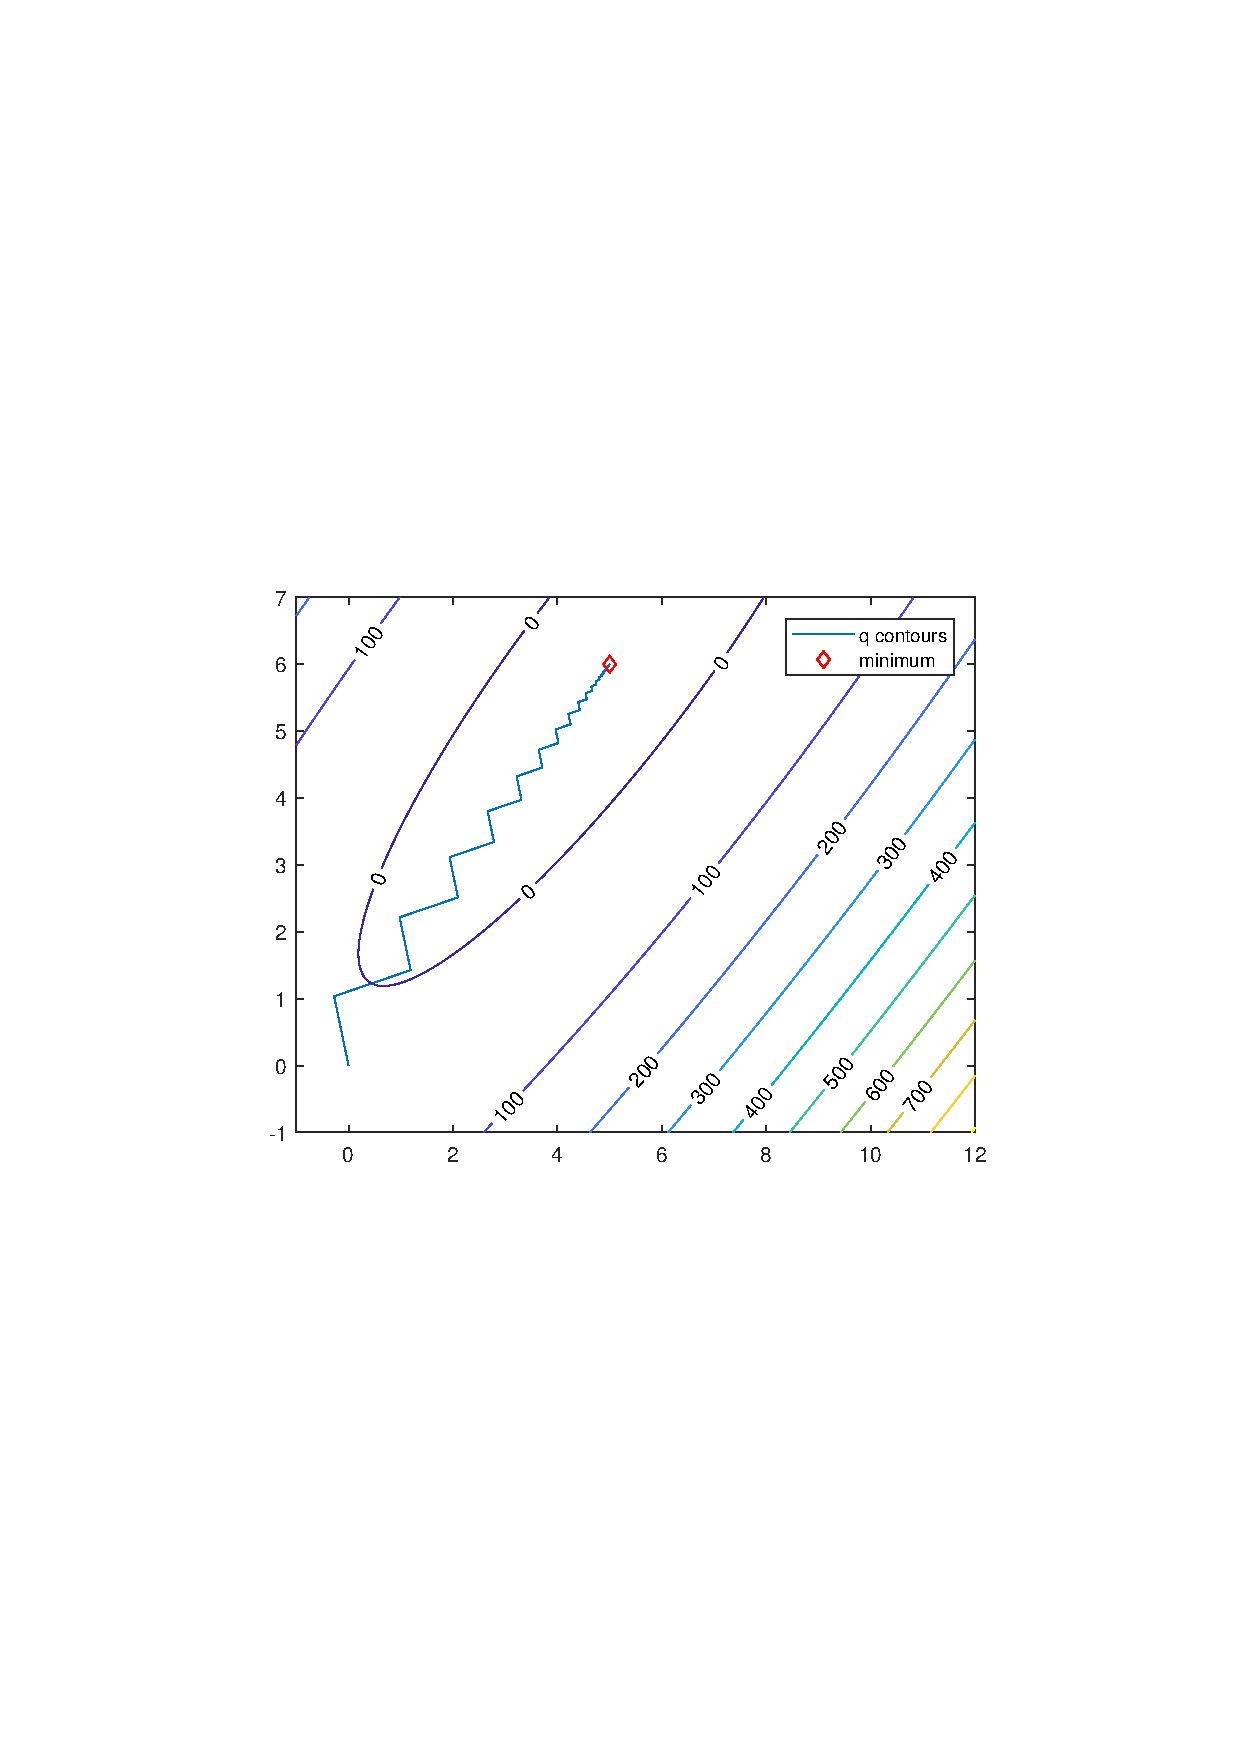
\includegraphics[width=5.7cm]{fig/1_1a.pdf}}
\subfigure{
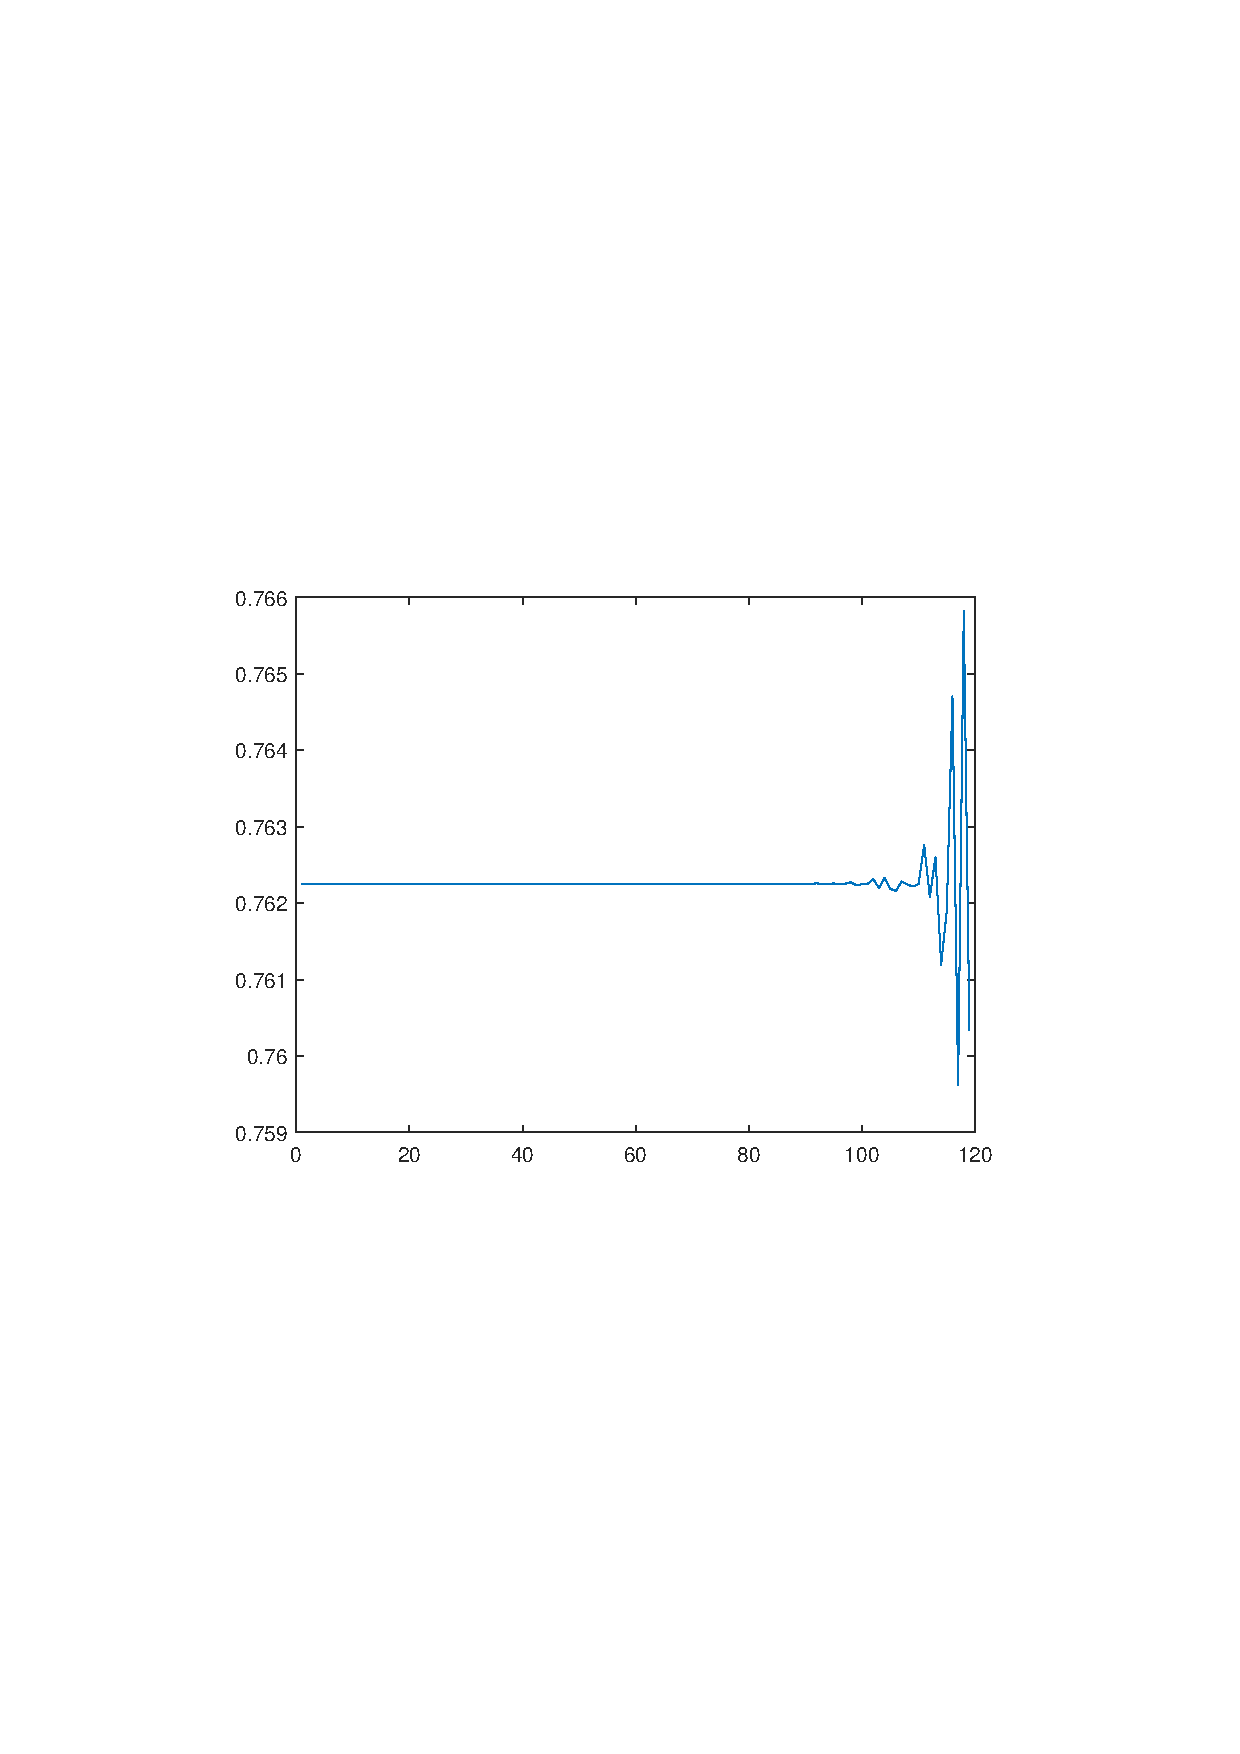
\includegraphics[width=6cm]{fig/1_1b.pdf}}
\caption{Steepest-denscent in (0,0)}
\label{Fig.lable}
\end{figure}

\begin{figure}[H]
\centering
\subfigure{
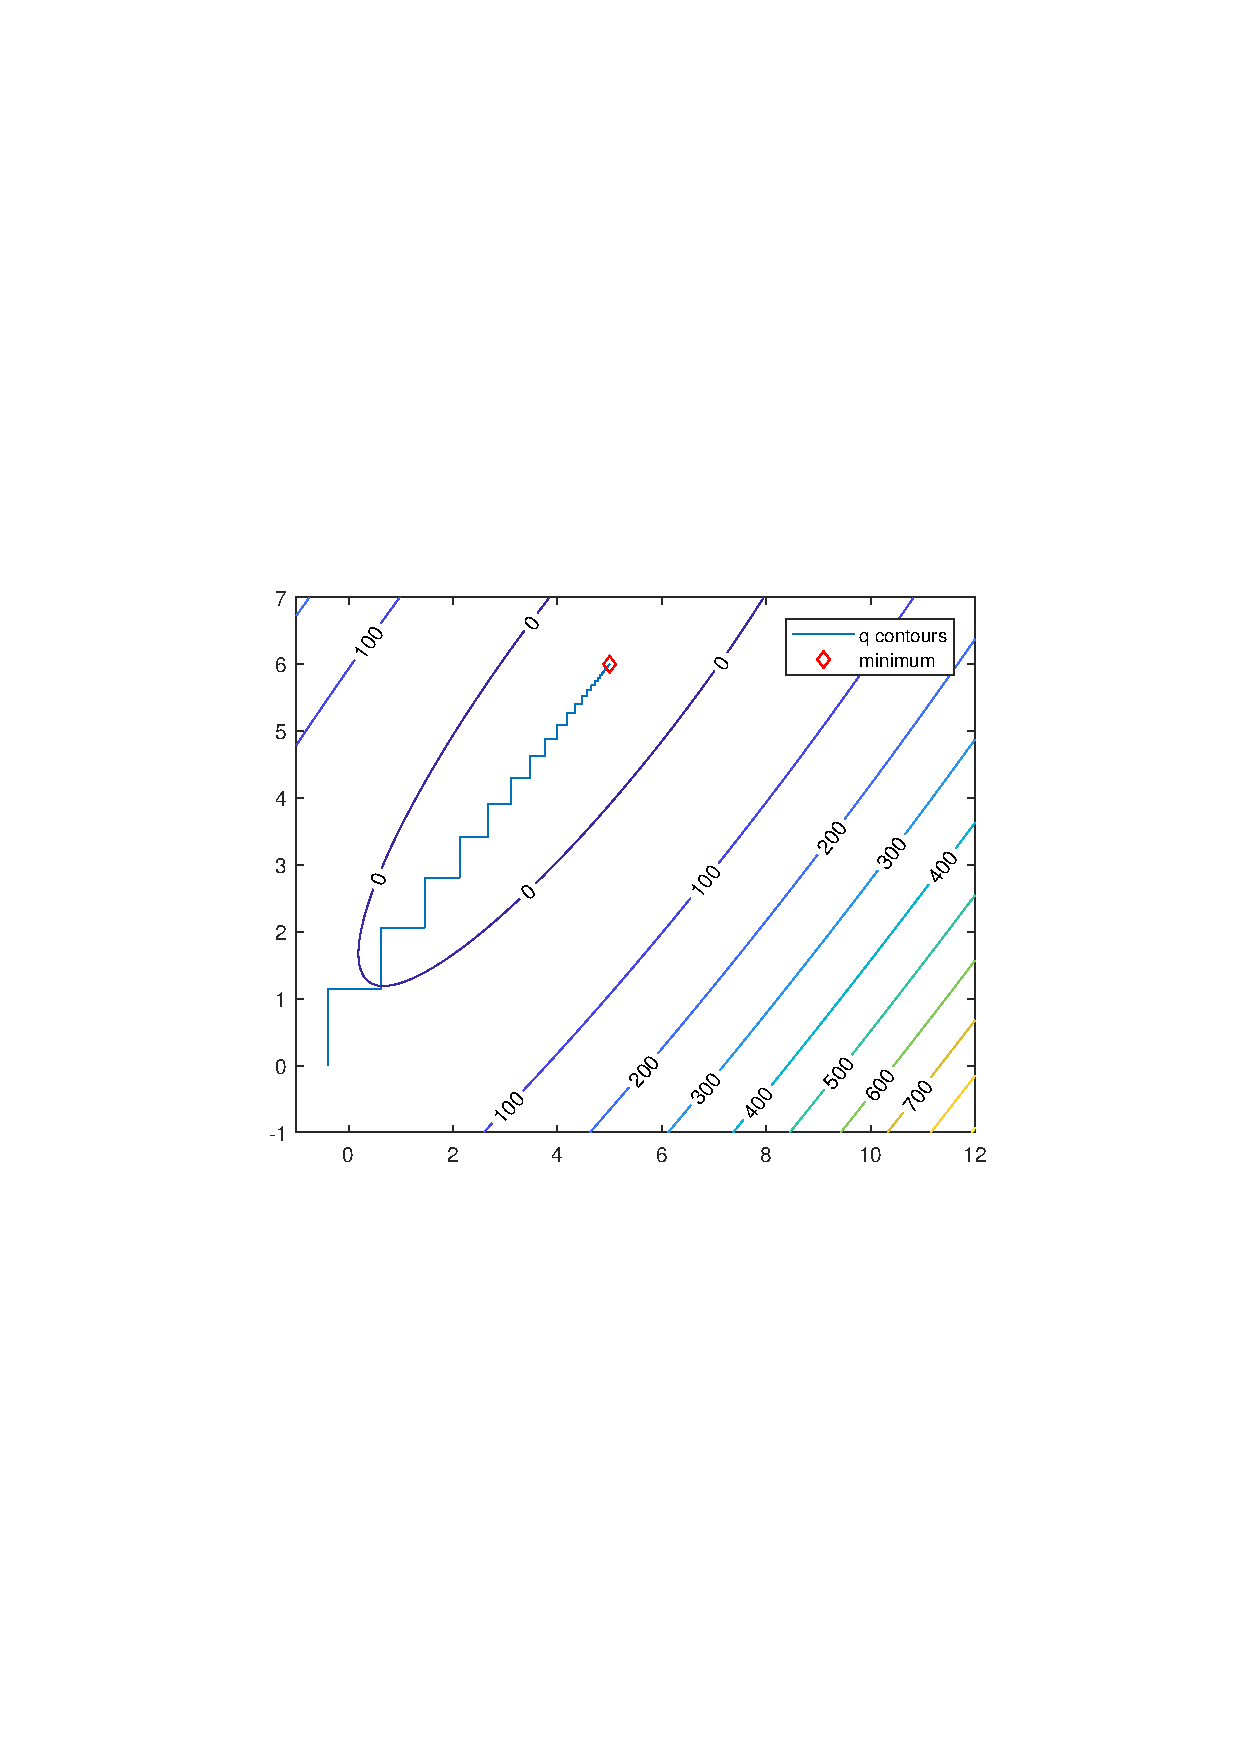
\includegraphics[width=5.7cm]{fig/1_2a.pdf}}
\subfigure{
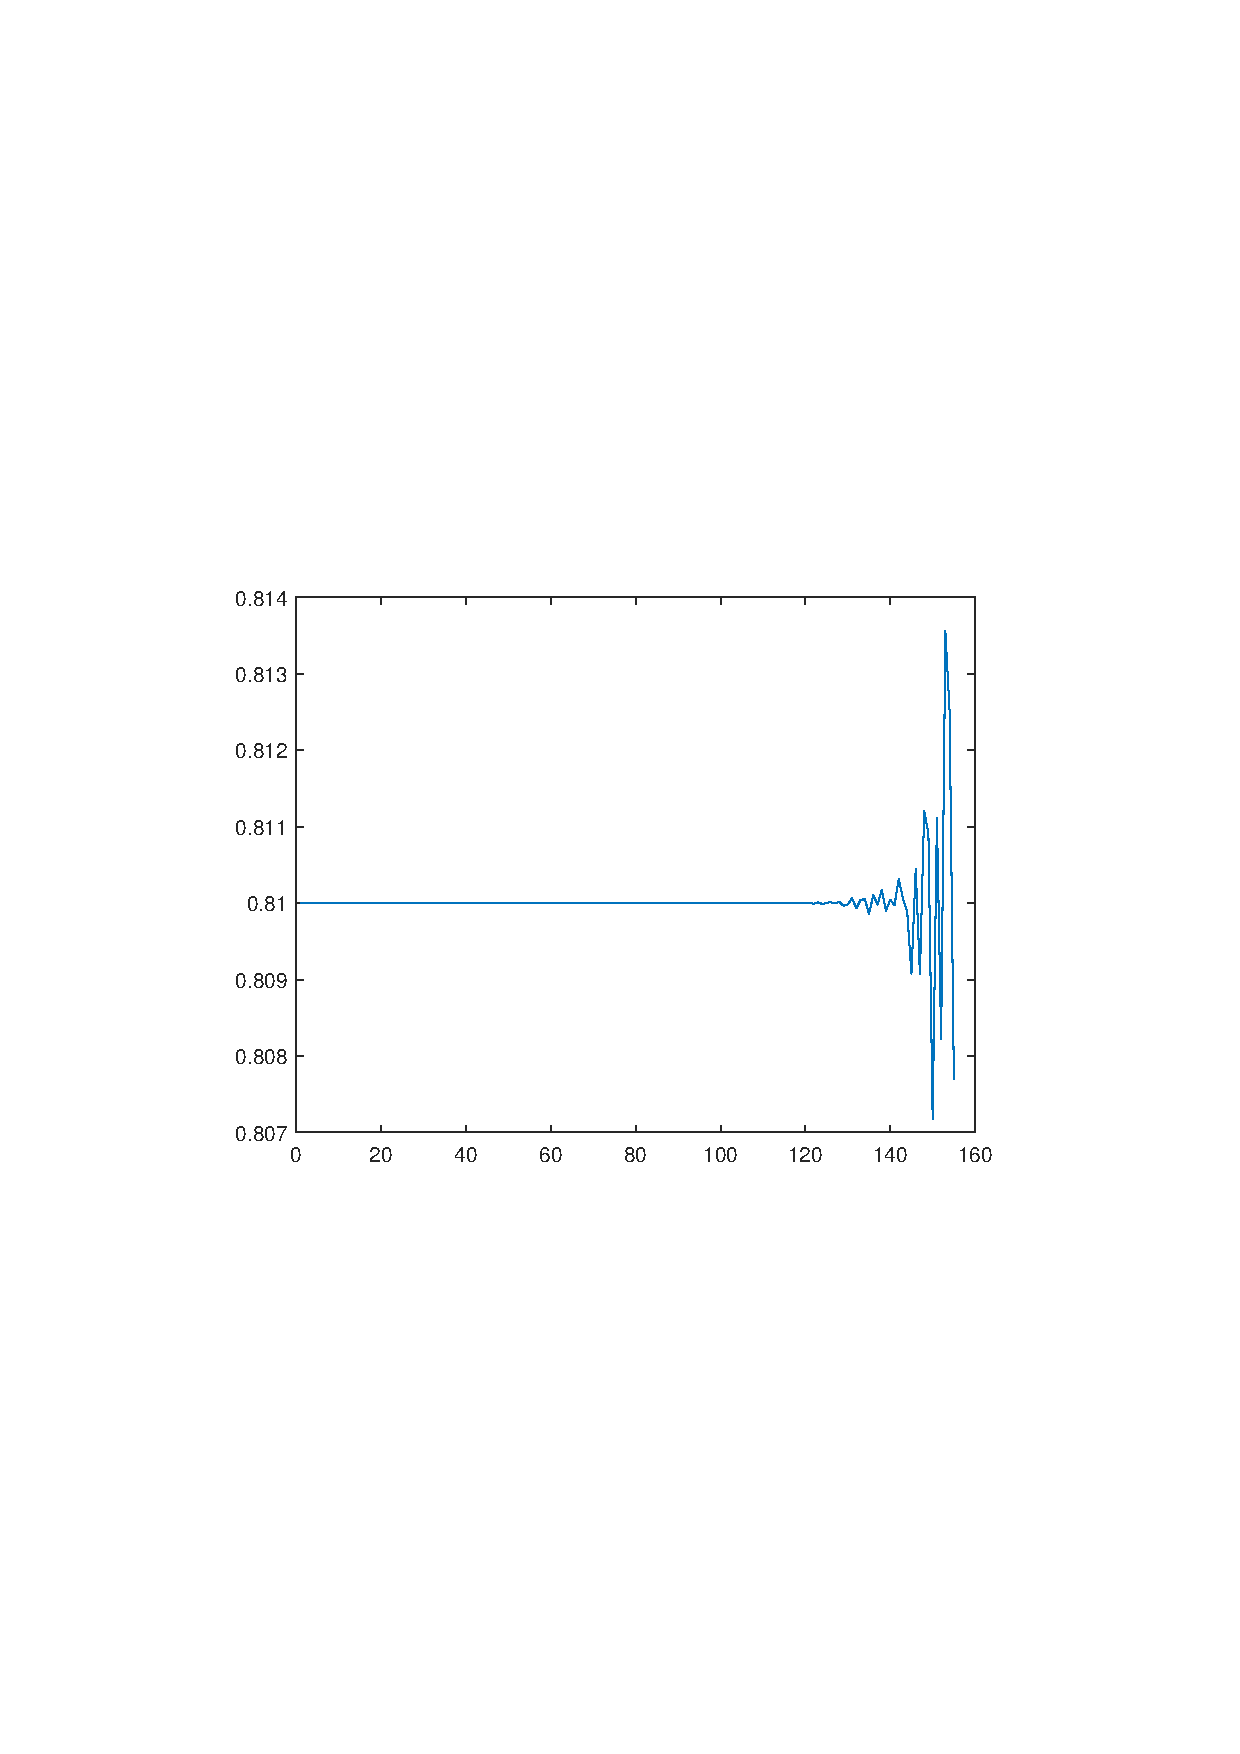
\includegraphics[width=6cm]{fig/1_2b.pdf}}
\caption{Steepest-denscent in (-0.4,0)}
\label{Fig.lable}
\end{figure}

\begin{figure}[H]
\centering
\subfigure{
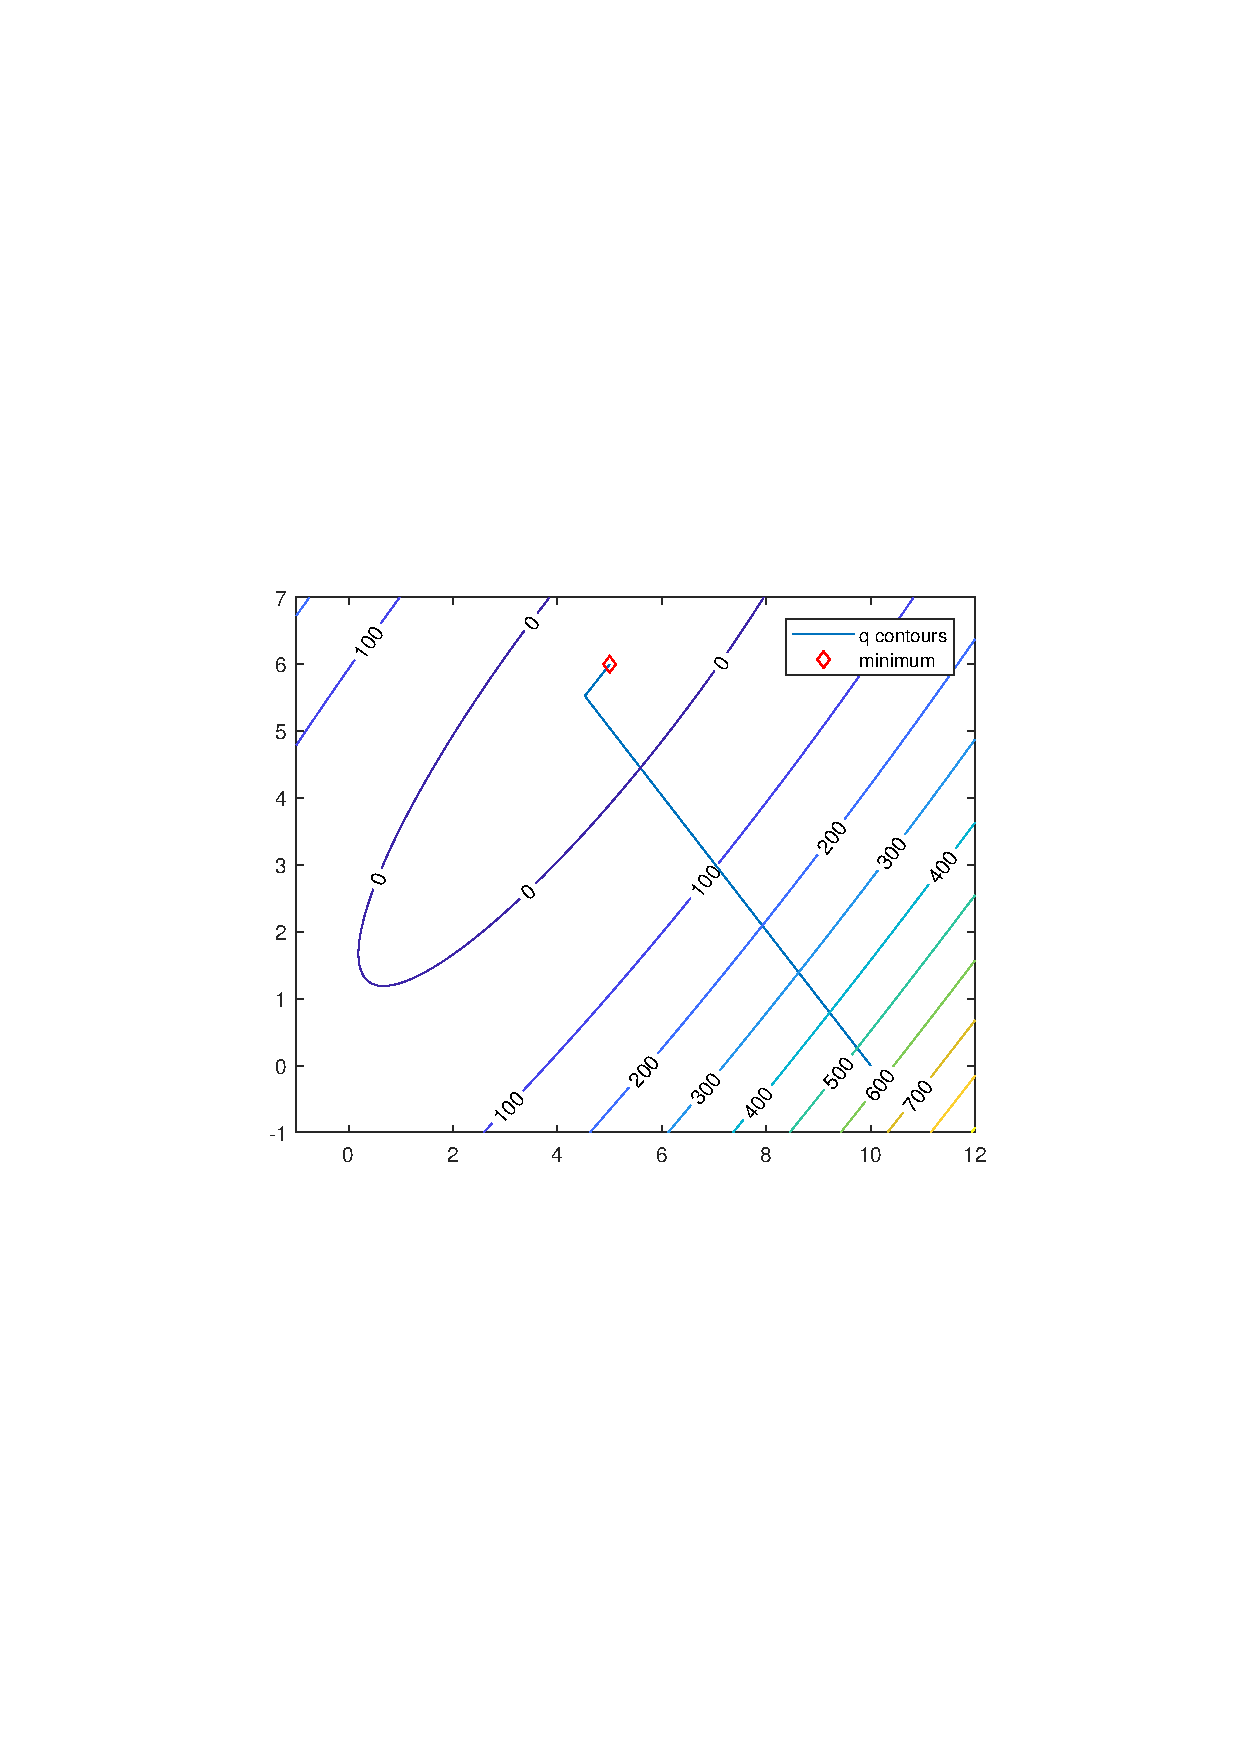
\includegraphics[width=5.7cm]{fig/1_3a.pdf}}
\subfigure{
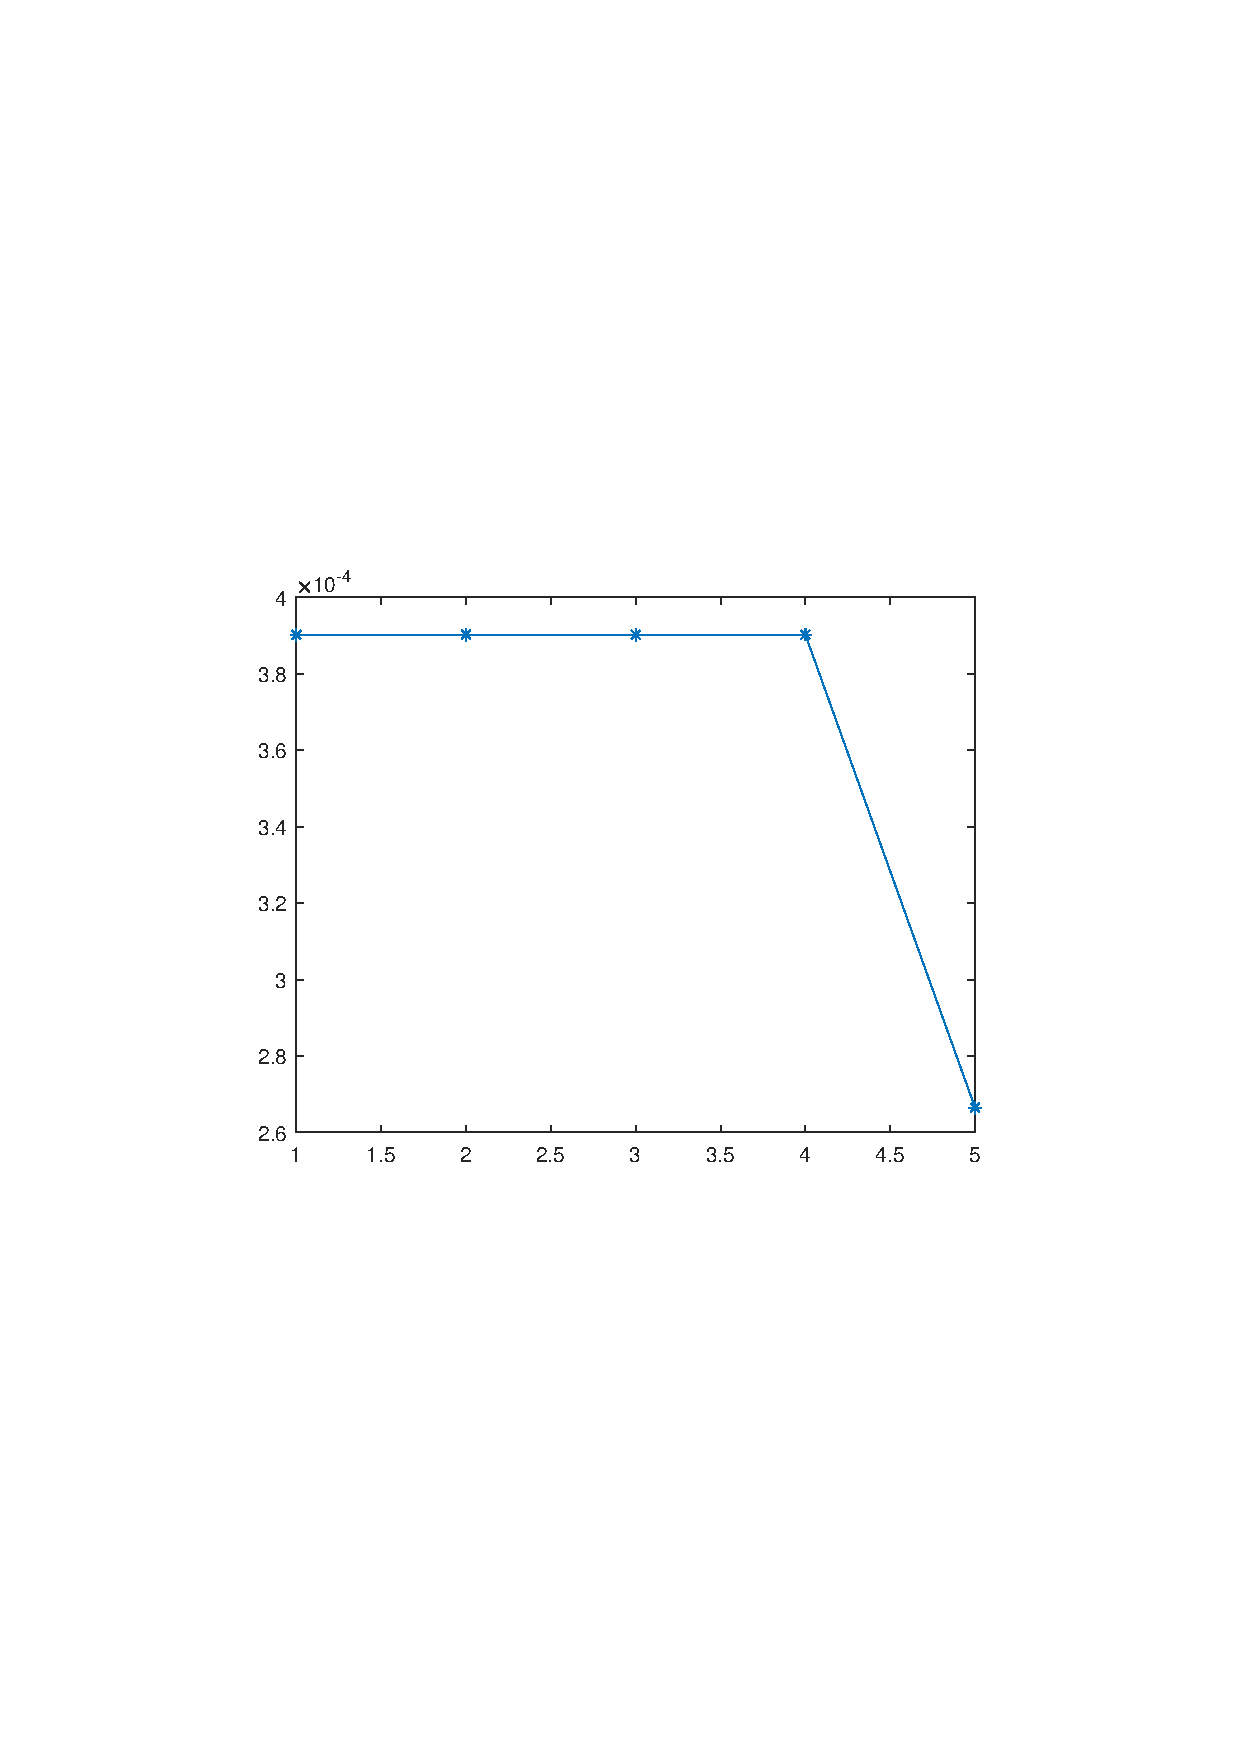
\includegraphics[width=5.8cm]{fig/1_3b.pdf}}
\caption{Steepest-denscent in (10,0)}
\label{Fig.lable}
\end{figure}

\begin{figure}[H]
\centering
\subfigure{
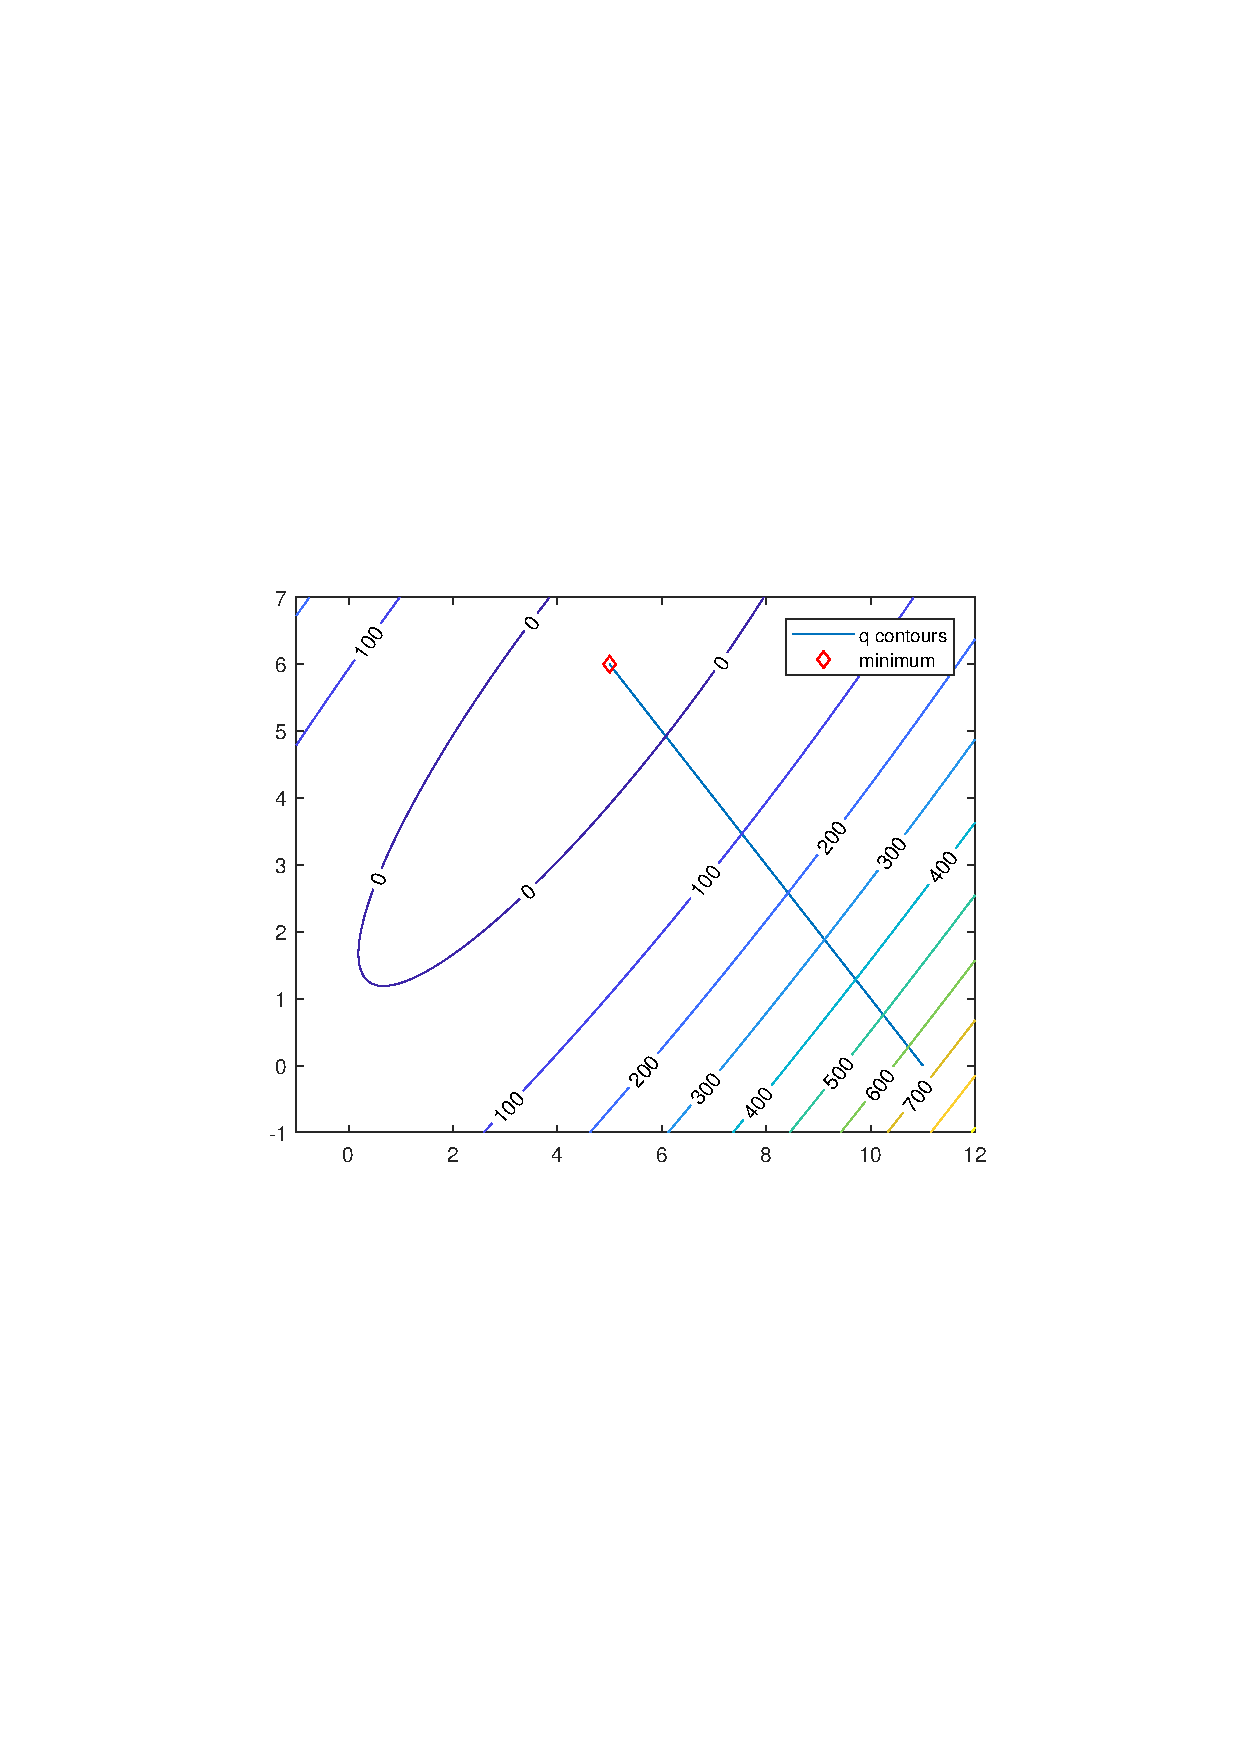
\includegraphics[width=5.8cm]{fig/1_4a.pdf}}
\subfigure{
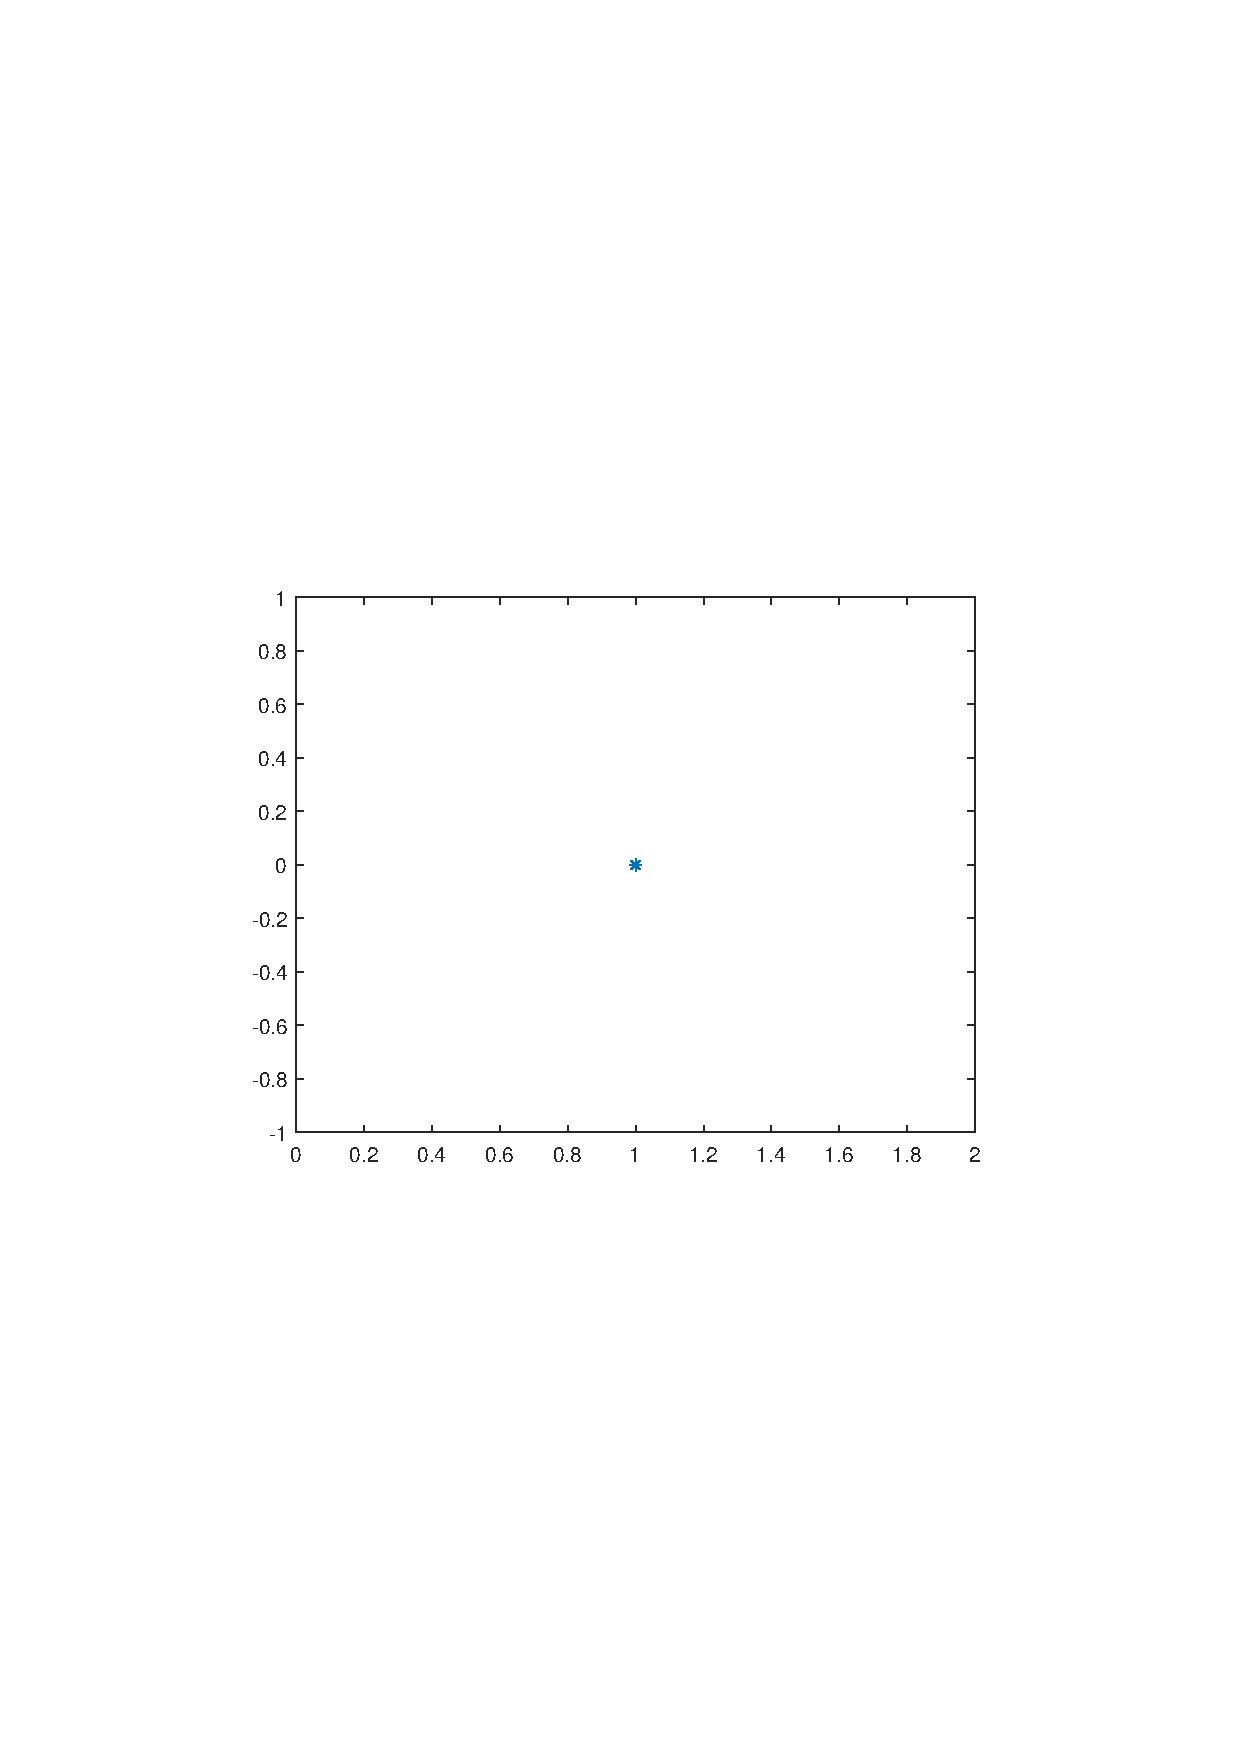
\includegraphics[width=5.9cm]{fig/1_4b.pdf}}

\caption{Steepest-denscent in (11,0)}
\label{Fig.lable}
\end{figure}

\begin{table}[H]
\centering
\caption{收敛因子比较}
	\begin{tabular}{ccccc}
	\toprule
	{起始点}&$(0,0)$&$(-0.4,0)$&$(10,0)$&$(11,0)$\\
	\midrule
	{收敛因子}&0.762255&0.810000&0.000390&0\\
	\bottomrule
	\end{tabular}
\end{table}

\subsection*{分析:}
由于目标函数为凸函数,故使用梯度下降法从这四个不同的起始点出发都能收敛到全局最优点,然而线性收敛因子却互不相同.

由图像可知:在迭代开始后,函数值的收敛速度稳定在一个值左右,直到接近最优点时,收敛速度开始较大幅度波动。

而且,可以看出,初始点越接近等值线椭圆的狭长端,线性收敛因子越大,在点$(-0.4,0)$处甚至达到了线性收敛因子的上界0.81,而离狭长端越远,收敛因子越小。
这是由于梯度下降在构造搜索方向时没有充分利用到函数的二阶导数信息,在面临“峡谷”状的函数时,会反复震荡到“峡谷”的另一端,而不能直接向最优值方向前进。

容易看出,等值线椭圆的长轴端斜率为$9/10$,且$(-0.4,0)=(5,6)-0.6*(9,10)$,这说明点$(-0.4,0)$刚好处在等值线椭圆的长轴上,因此也是震荡最剧烈的地方,收敛速度达到了最坏收敛速度。


\section{5.7}

\begin{algorithm}[h]  
\caption{Newton method for problem(5.7)}  
\begin{algorithmic}[1]  
\STATE Given $x^{(0)}$ and compute $g(x)=f'(x)$
\STATE Compute $G(x)=g'(x)$
\STATE Set $g^{(0)}=g(x^{(0)}),k=0$
\WHILE {$|g^{(k)}|>\epsilon$}
\STATE Set $s^{(k)}=-g^{(k)}/G^{(k)}$
\STATE Set $x^{(k+1)}=x^{(k)}+s^{(k)}$
\STATE Set k=k+1
\ENDWHILE
\end{algorithmic}  
\end{algorithm}  

其中:\[g(x)=f'(x)=9-\dfrac{4}{x-7}\]
\[G(x)=g'(x)=\dfrac{4}{(x-7)^2}\]
\[x^{(k+1)}=x^{(k)}-\dfrac{1}{4}(x^{(k)}-7)(9x^{(k)}-67)\]

% Table generated by Excel2LaTeX from sheet 'Sheet1'
\begin{table}[htbp]
  \centering
  \caption{迭代5次过程}
    \begin{tabular}{clllll}
\toprule
  $x^{(0)}$&7.4  & 7.2  & 7.01 &7.80  & 7.88 \\
	\midrule
   $x^{(1)}$& 7.44  & 7.31  & 7.019775 & 7.16  & 7.0176 \\
    $x^{(2)}$&7.4444 & 7.403775 & 7.038670136 & 7.2624 & 7.03450304 \\
    $x^{(3)}$&7.44444444 & 7.440722936 & 7.073975668 & 7.36987904 & 7.066327546 \\
   $ x^{(4)}$&7.444444444 & 7.444413283 & 7.135638438 & 7.431934445 & 7.122756569 \\
    $x^{(5)}$&7.444444444 & 7.444444442 & 7.229881858 & 7.444092319 & 7.211607493 \\
	\midrule
    $f(x^{(5)})$&70.24372086 & 70.24372086 & 70.94969577 & 70.24372212 & 71.11655611 \\
	\bottomrule
    \end{tabular}%
  \label{tab:addlabel}%
\end{table}%
由MATLAB函数fminsearch求得最优解为:\[x^{\star}=7.444421386718750,\quad f(x^{\star})=70.243720870248540\]

\begin{figure}[H]
\centering
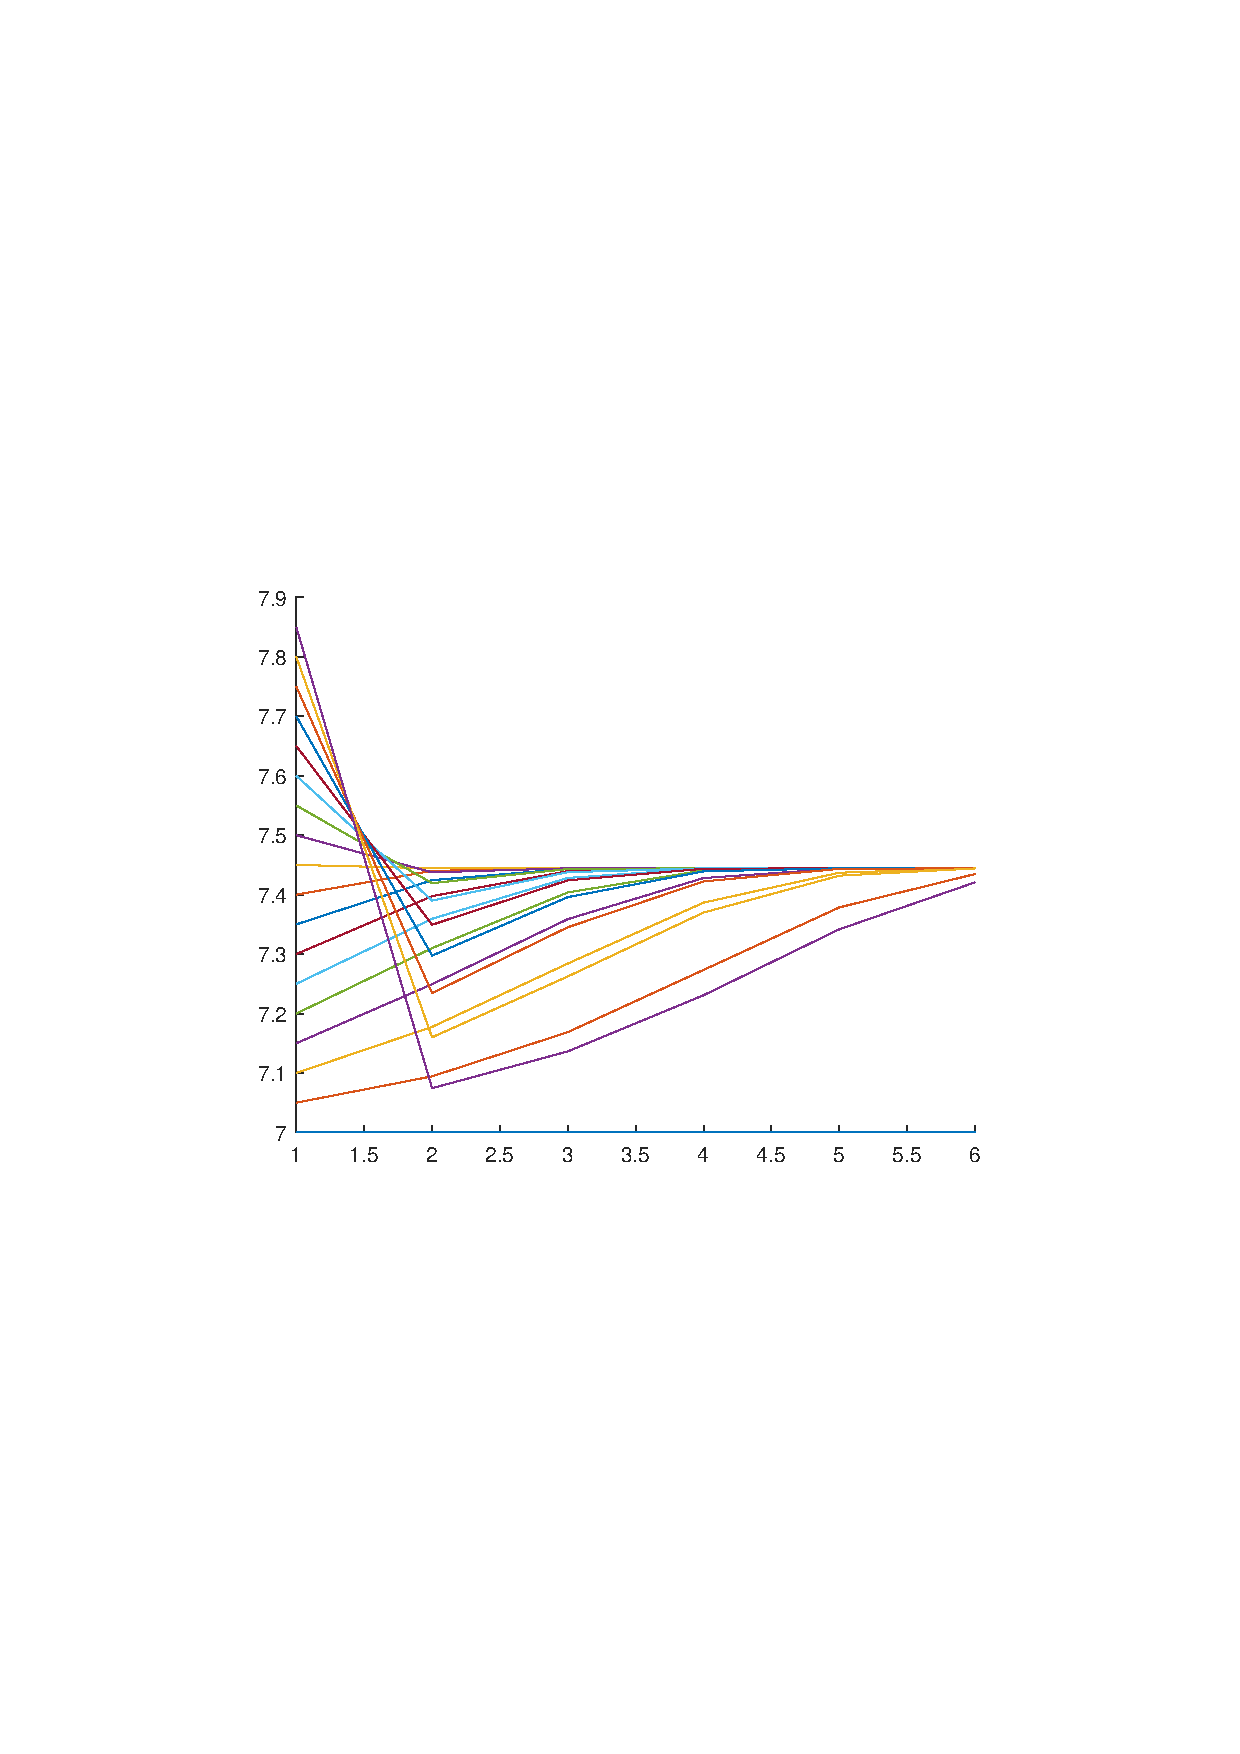
\includegraphics[width=11cm]{fig/2_1.pdf}
\end{figure}

\begin{figure}[H]
\centering
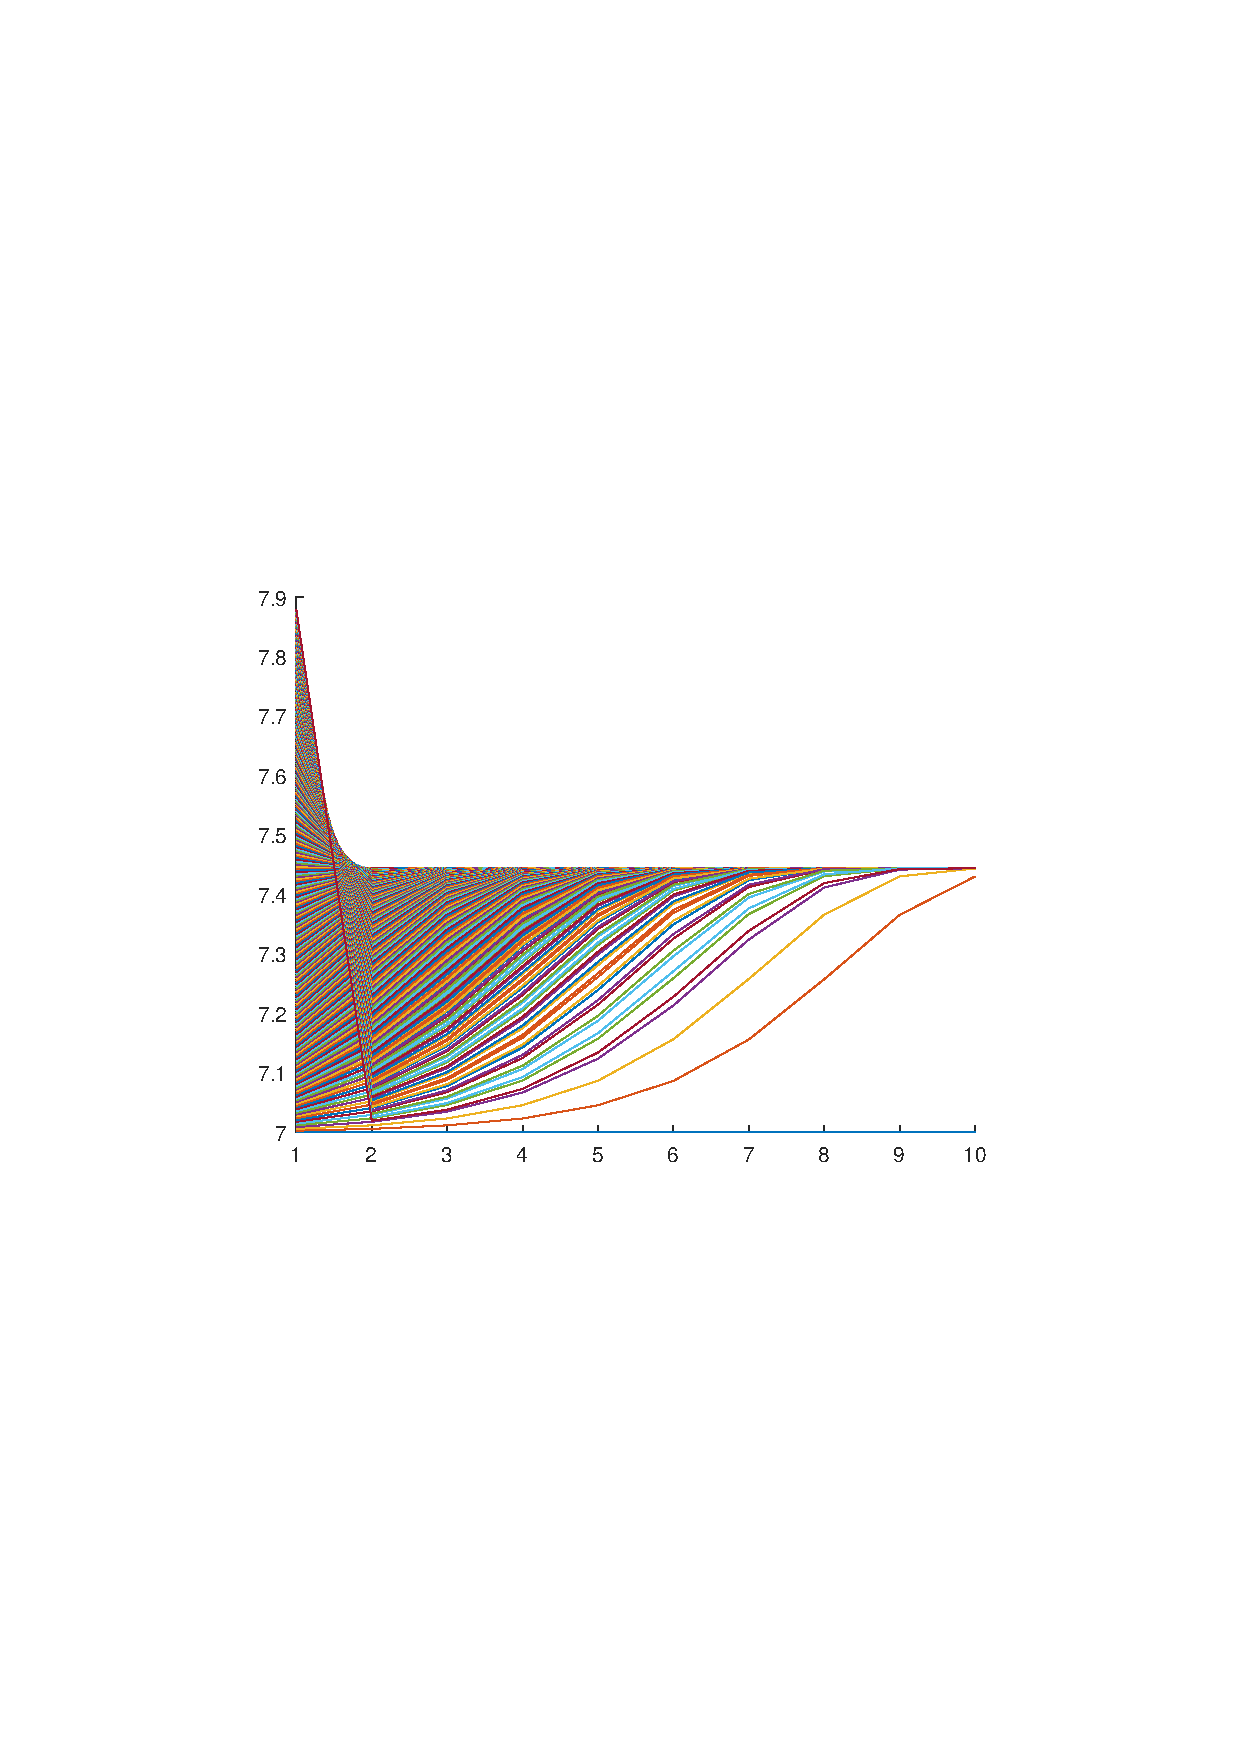
\includegraphics[width=11cm]{fig/2_2.pdf}
\end{figure}

\section{5.8}
\[f({x_1},{x_2}){:=}-9{x_1}-10{x_2}-\mu \left[\ln(-{x_1}-{x_2}+100)+\ln (-{x_1}+{x_2}+50)+\ln ({x_1})+\ln ({x_2})\right]\]

\[
g(x_1, x_2) = \nabla f(x_1, x_2)=
\begin{bmatrix}
-9 -\dfrac{\mu}{x_1 }+\dfrac{\mu}{100 - x_1 - x_2} + \dfrac{\mu}{50 - x_1 + x_2} \\
-10 - \dfrac{\mu}{x_2 }+\dfrac{\mu}{100 - x_1 - x_2} - \dfrac{\mu}{50 - x_1 + x_2}
\end{bmatrix}
\]


\[G[x_1, x_2] = \nabla g(x_1, x_2)=\]
\[
\begin{bmatrix}
\dfrac{1}{{x_1}^2 }+\dfrac{1}{(100 - x_1 - x_2)^2} + \dfrac{1}{(50 - x_1 + x_2)^2} 
&\dfrac{1}{(100 - x_1 - x_2)^2} - \dfrac{1}{(50 - x_1 + x_2)^2}\\
\dfrac{1}{(100 - x_1 - x_2)^2} - \dfrac{1}{(50 - x_1 + x_2)^2}&
\dfrac{1}{{x_2}^2 }+\dfrac{1}{(100 - x_1 - x_2)^2} + \dfrac{1}{(50 - x_1 + x_2)^2} 
\end{bmatrix}
\]

\begin{figure}[H]
\centering
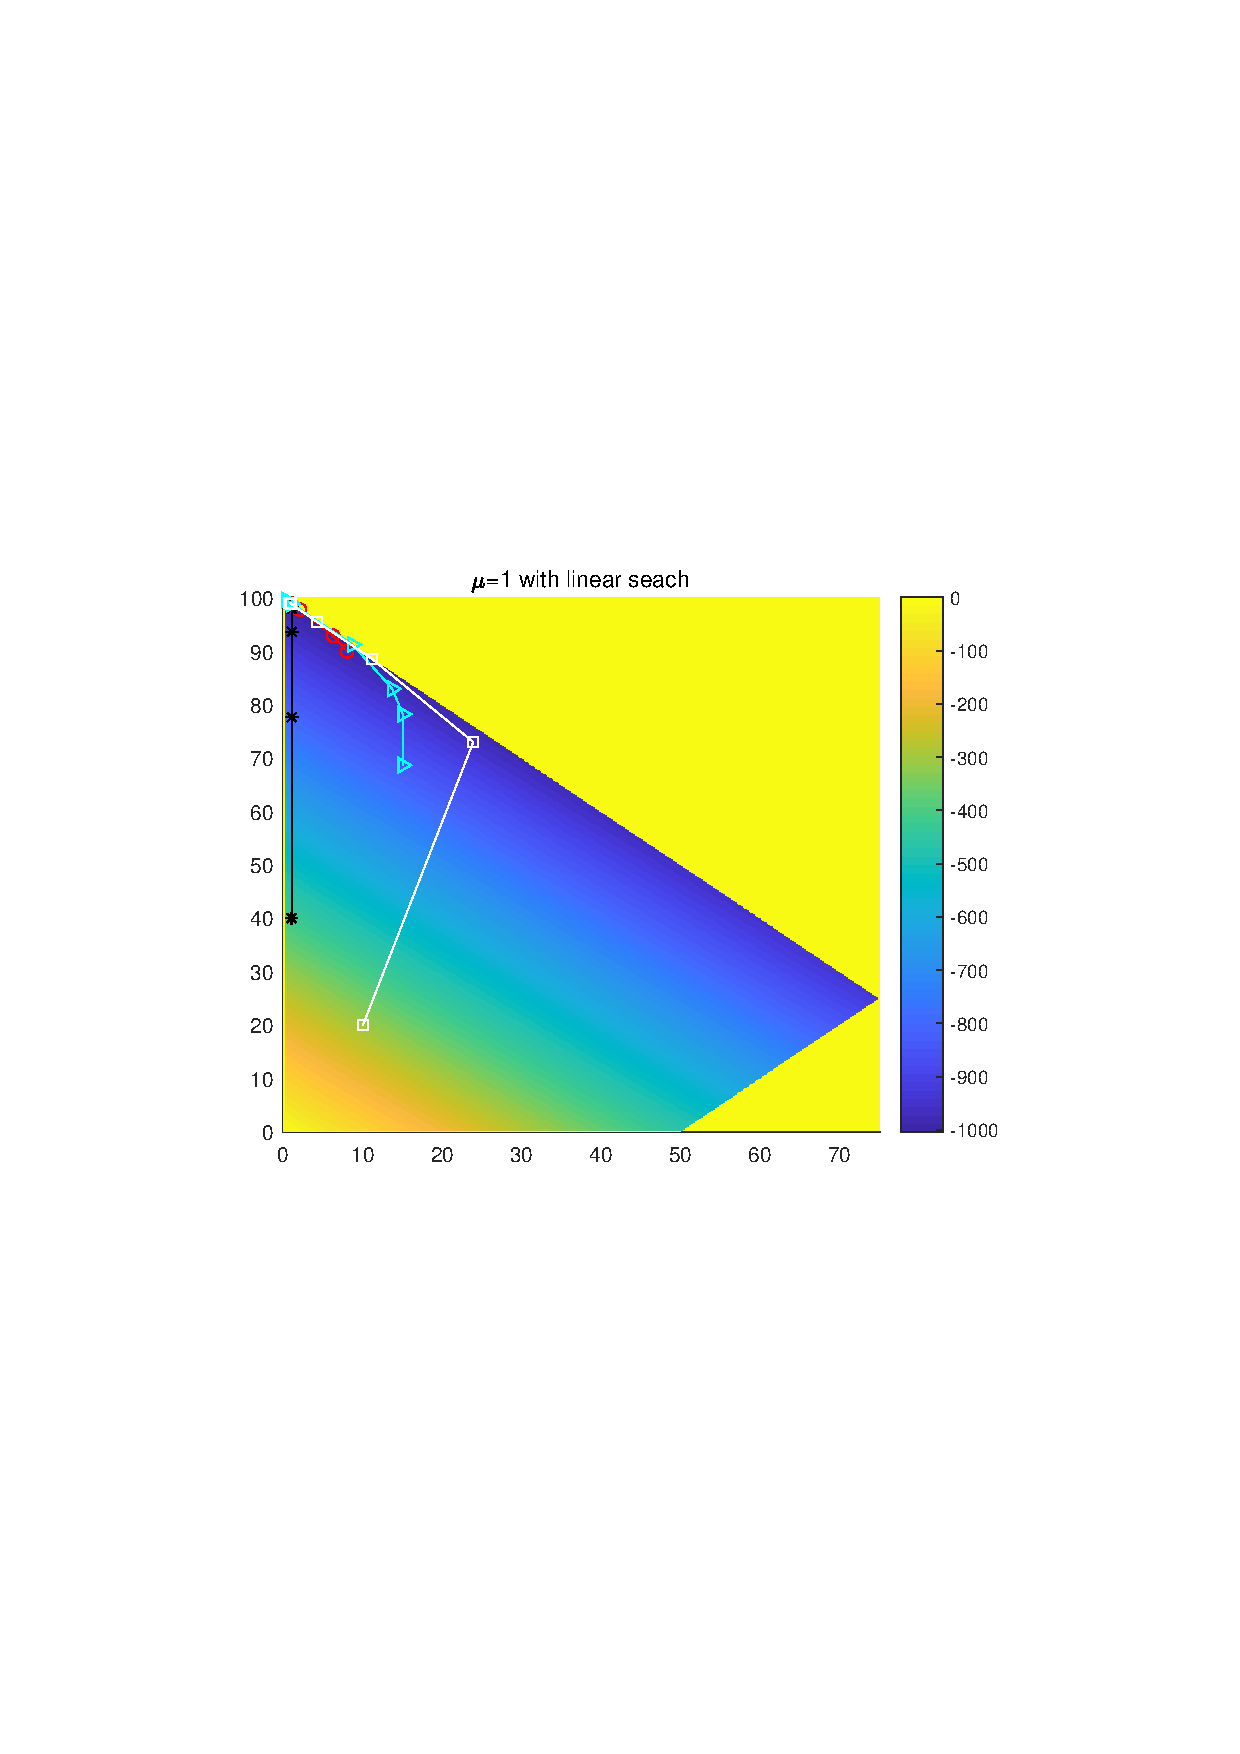
\includegraphics[width=11cm]{fig/5_1.pdf}
\end{figure}

\begin{figure}[H]
\centering
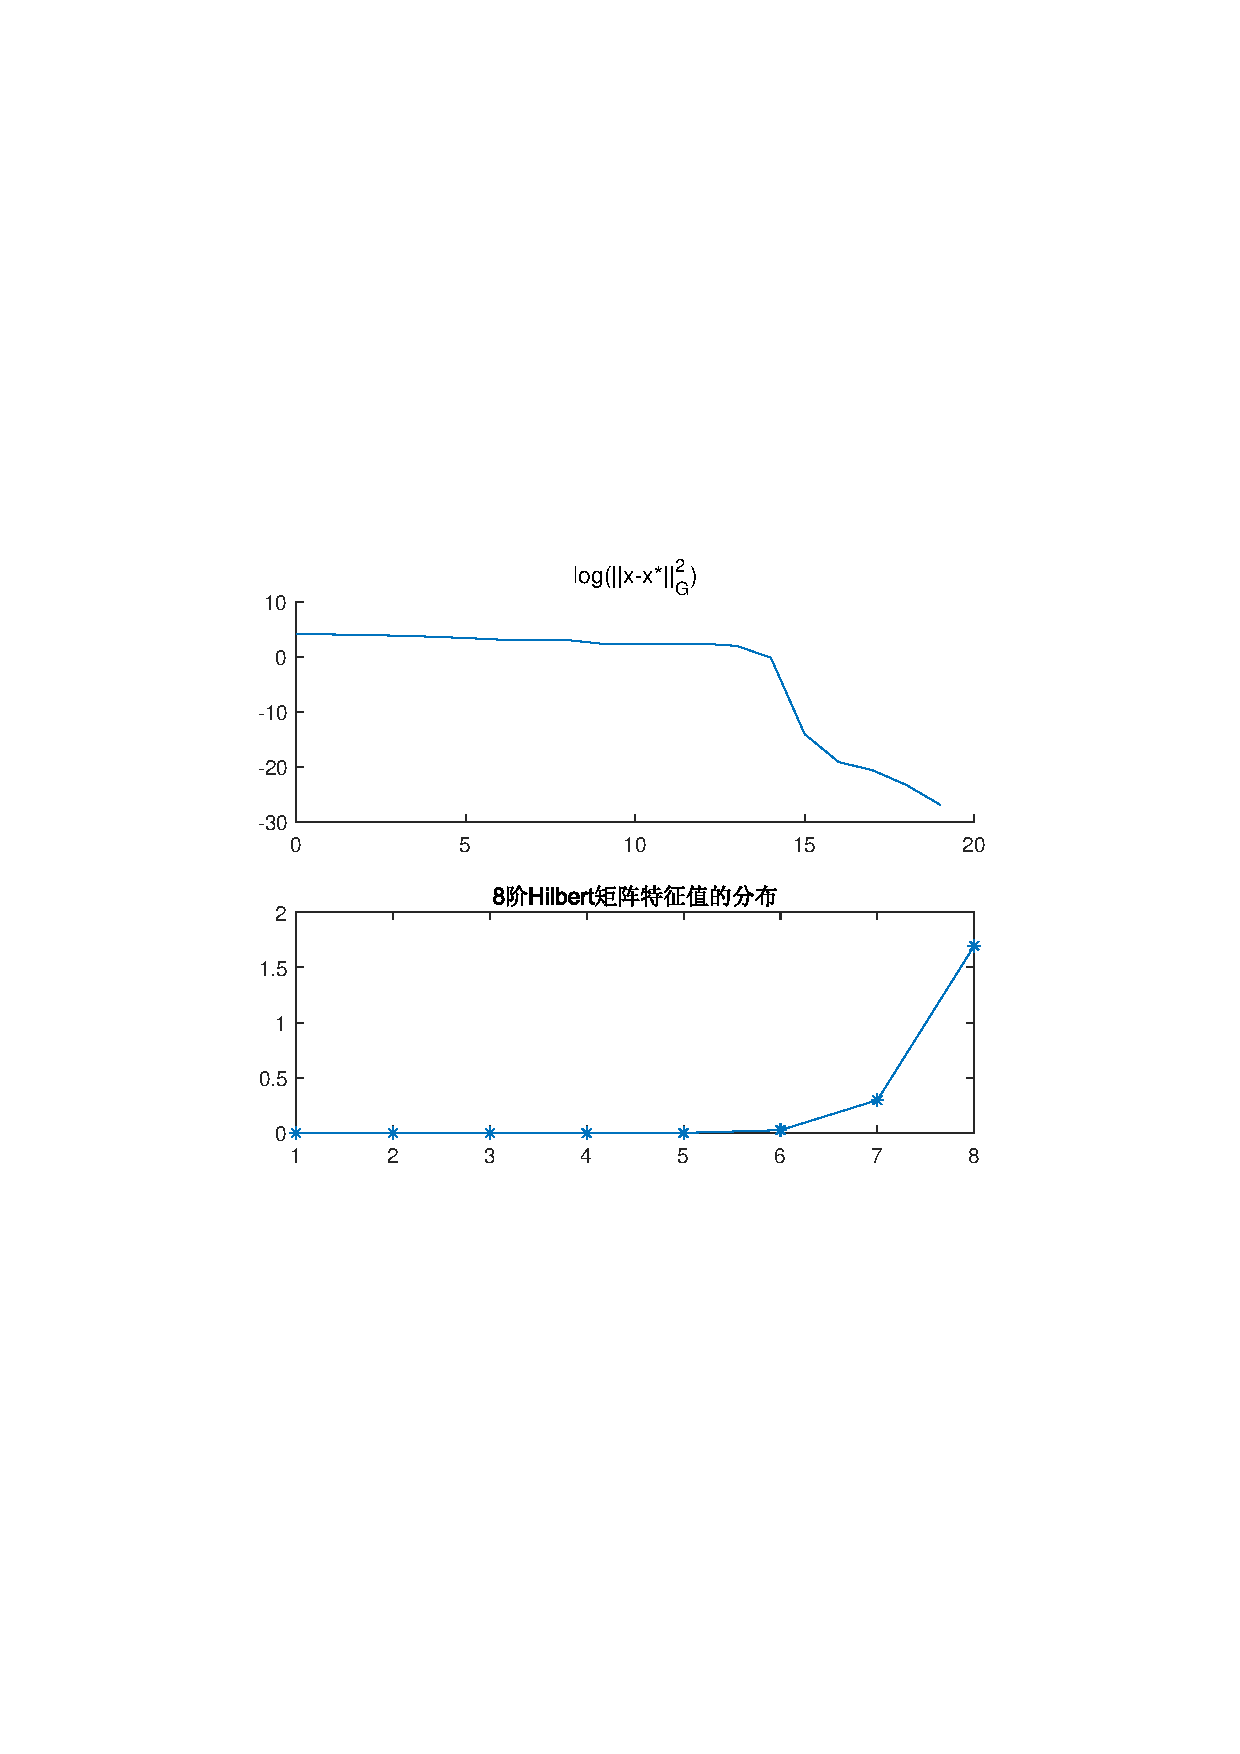
\includegraphics[width=11cm]{fig/5_2.pdf}
\end{figure}



\section{5.9}
首先画出Rosenbrock函数的图像及等值线如下\footnote{由于Rosenbrock函数过于陡峭,因此对原函数进行了取对数处理,以便于观察其特点。}:


\begin{figure}[H]
\centering
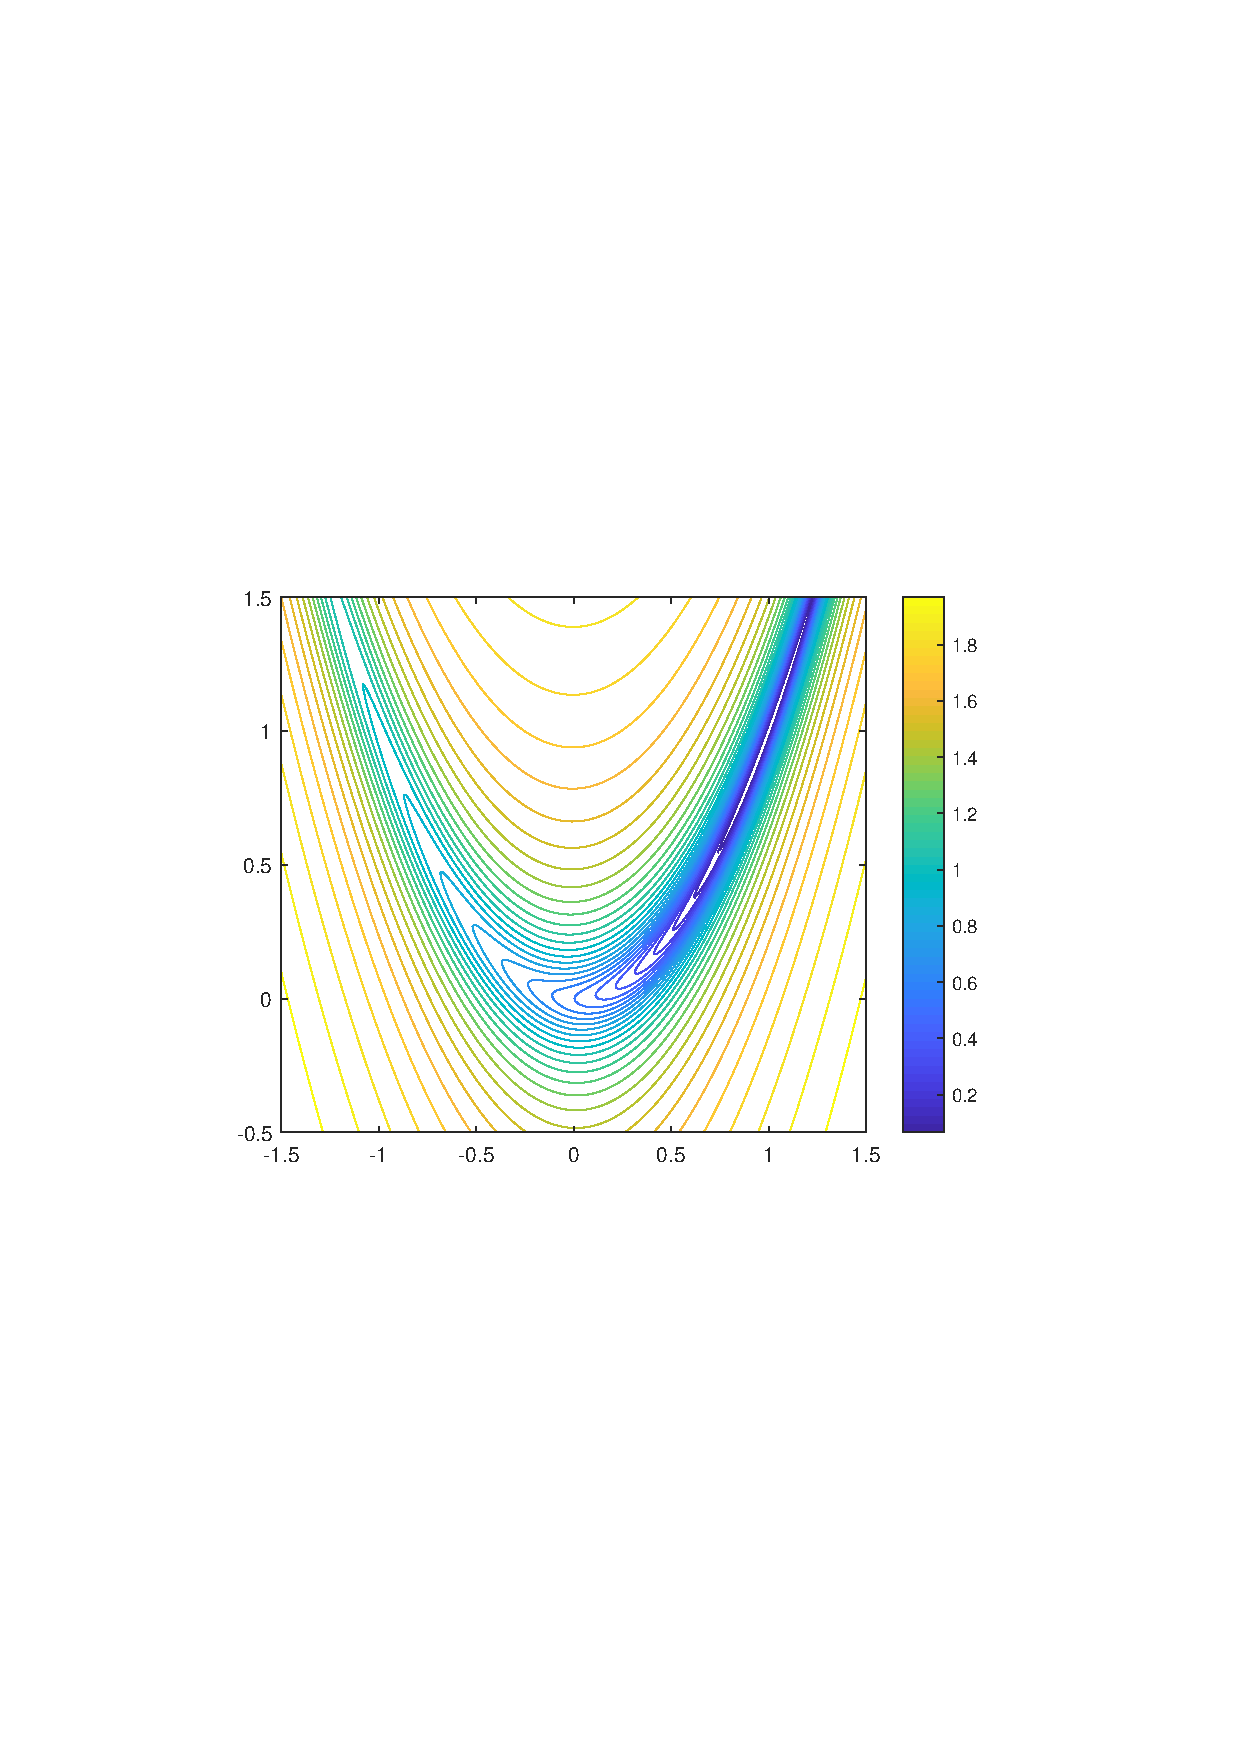
\includegraphics[width=11cm]{fig/4_01.pdf}
\end{figure}


\begin{figure}[H]
\centering
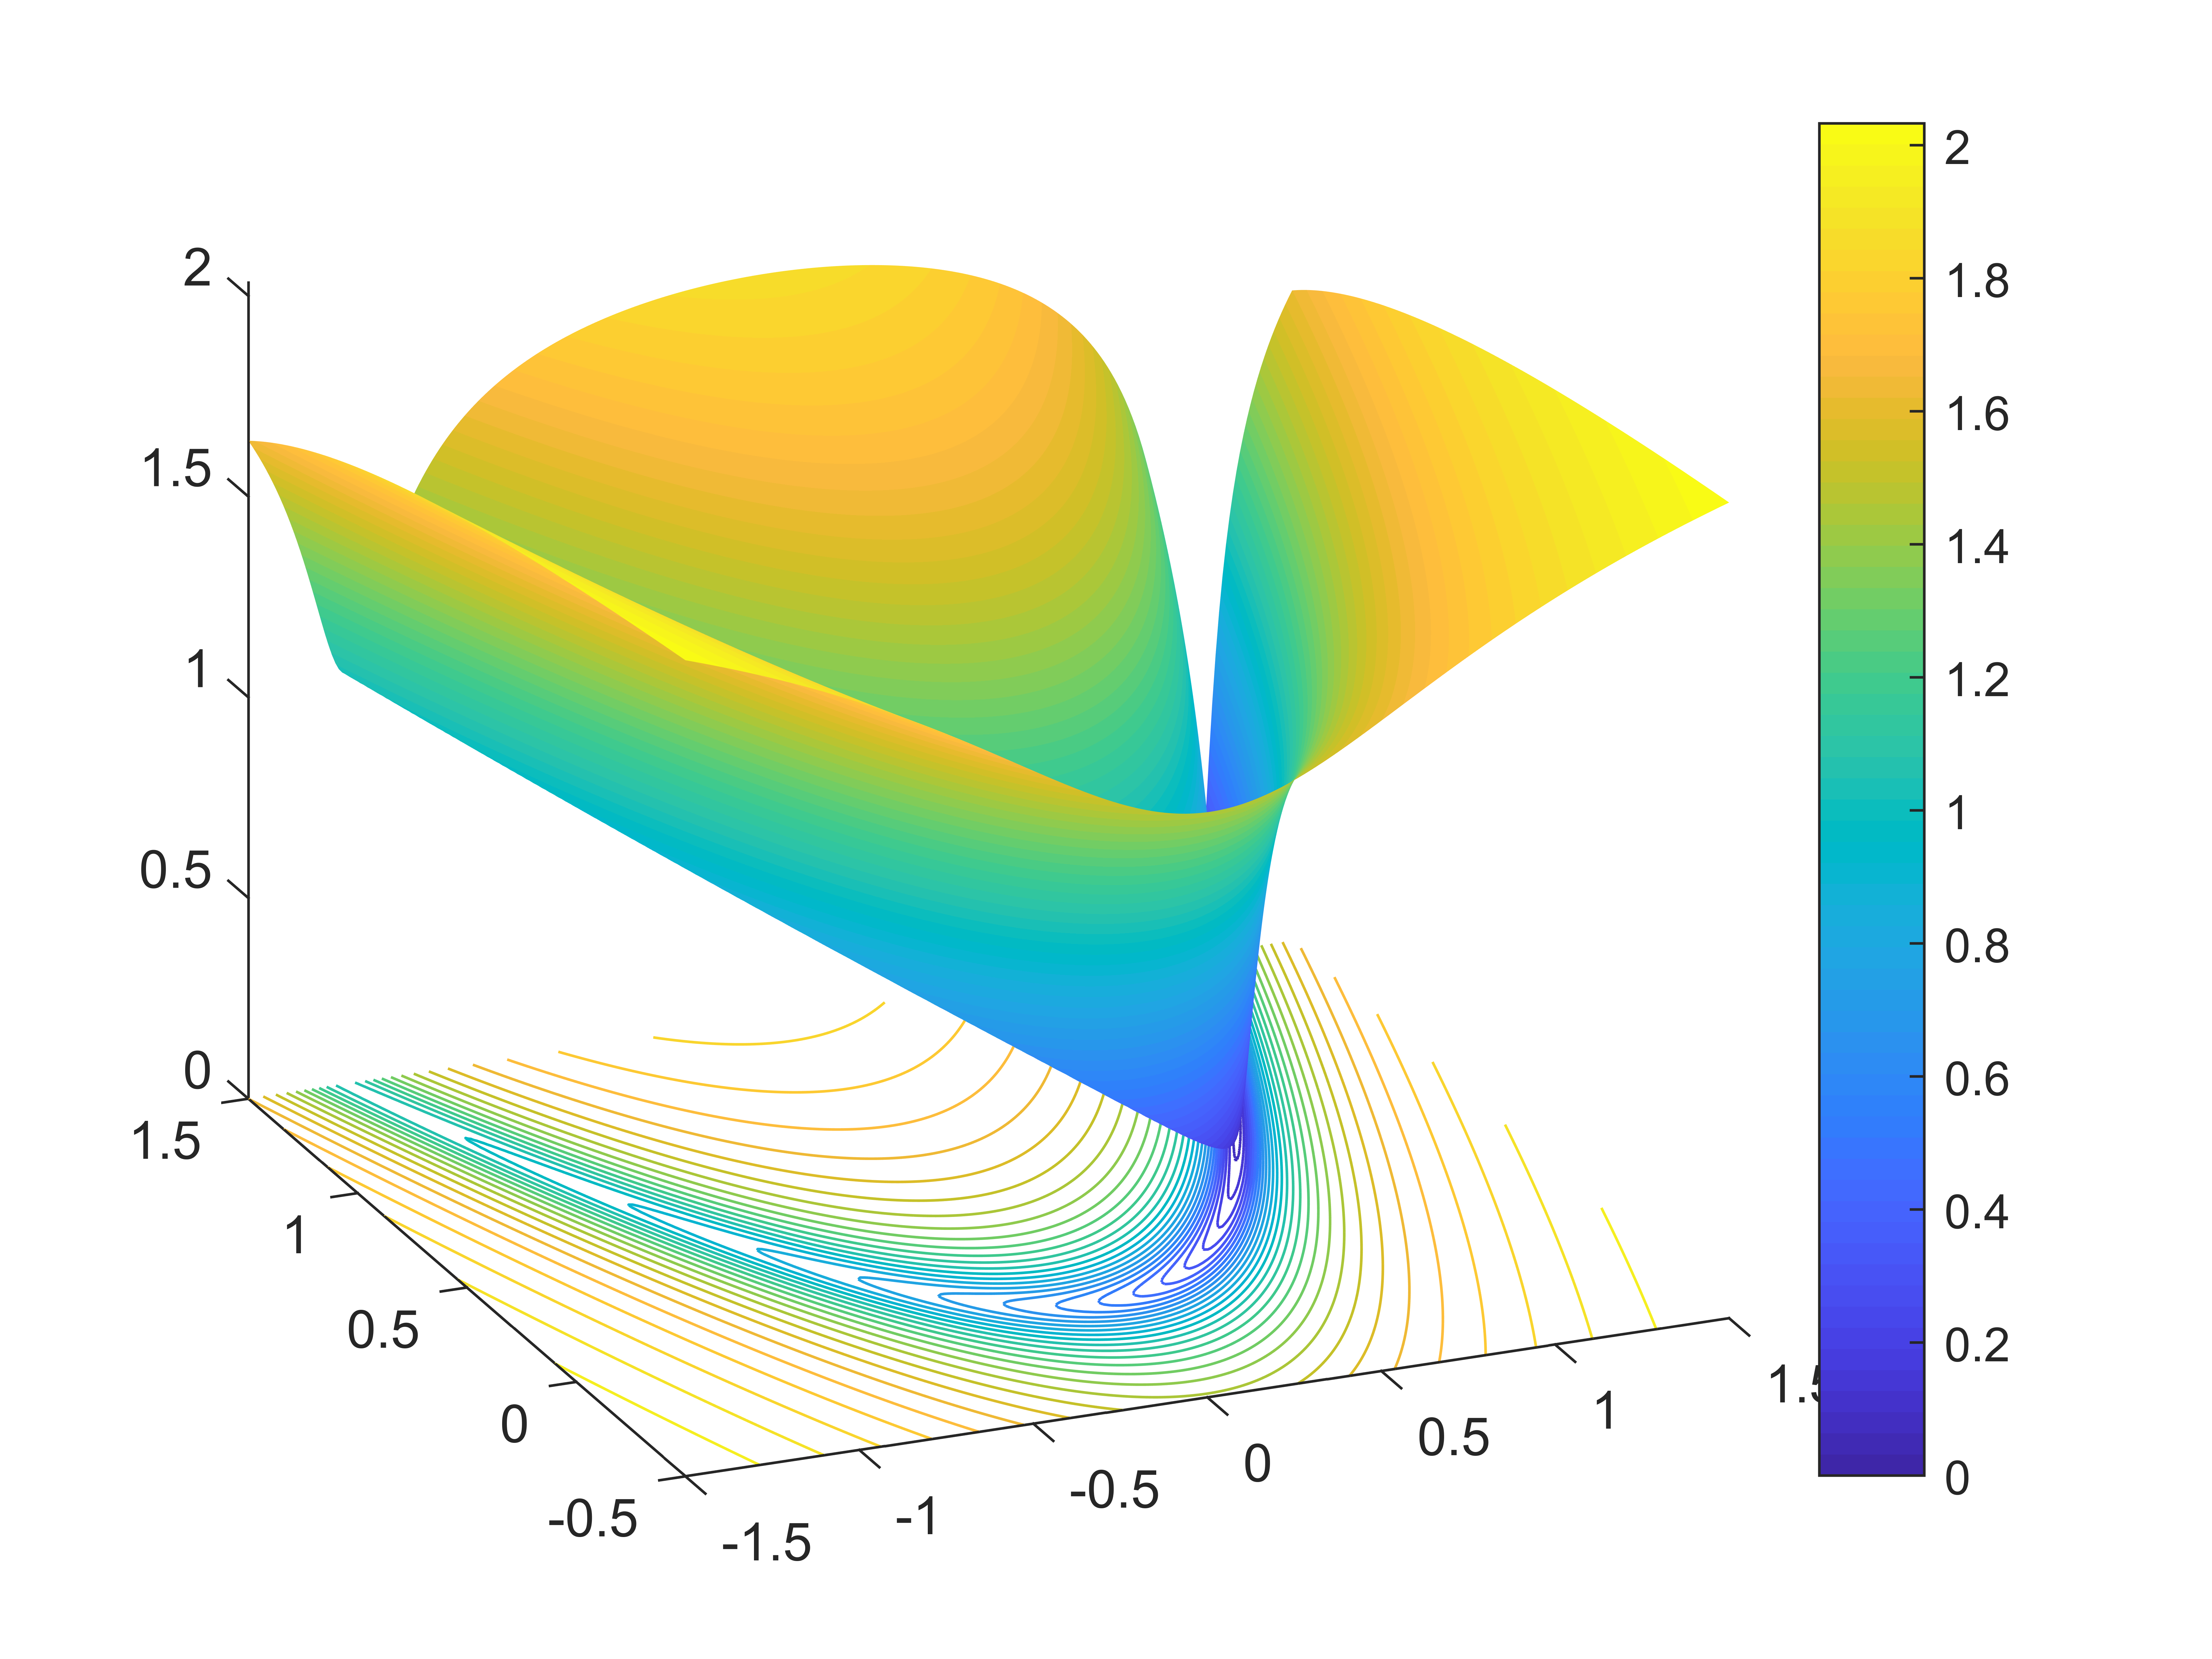
\includegraphics[width=11cm]{fig/4_02.png}
\end{figure}

本题中Armijo线搜索的参数为$\gamma=0.5,\rho=0.01$.

然后分别以梯度下降法和牛顿法迭代,并画出等高线、运动轨迹、迭代值如下:

\begin{figure}[H]
\centering
\subfigure{
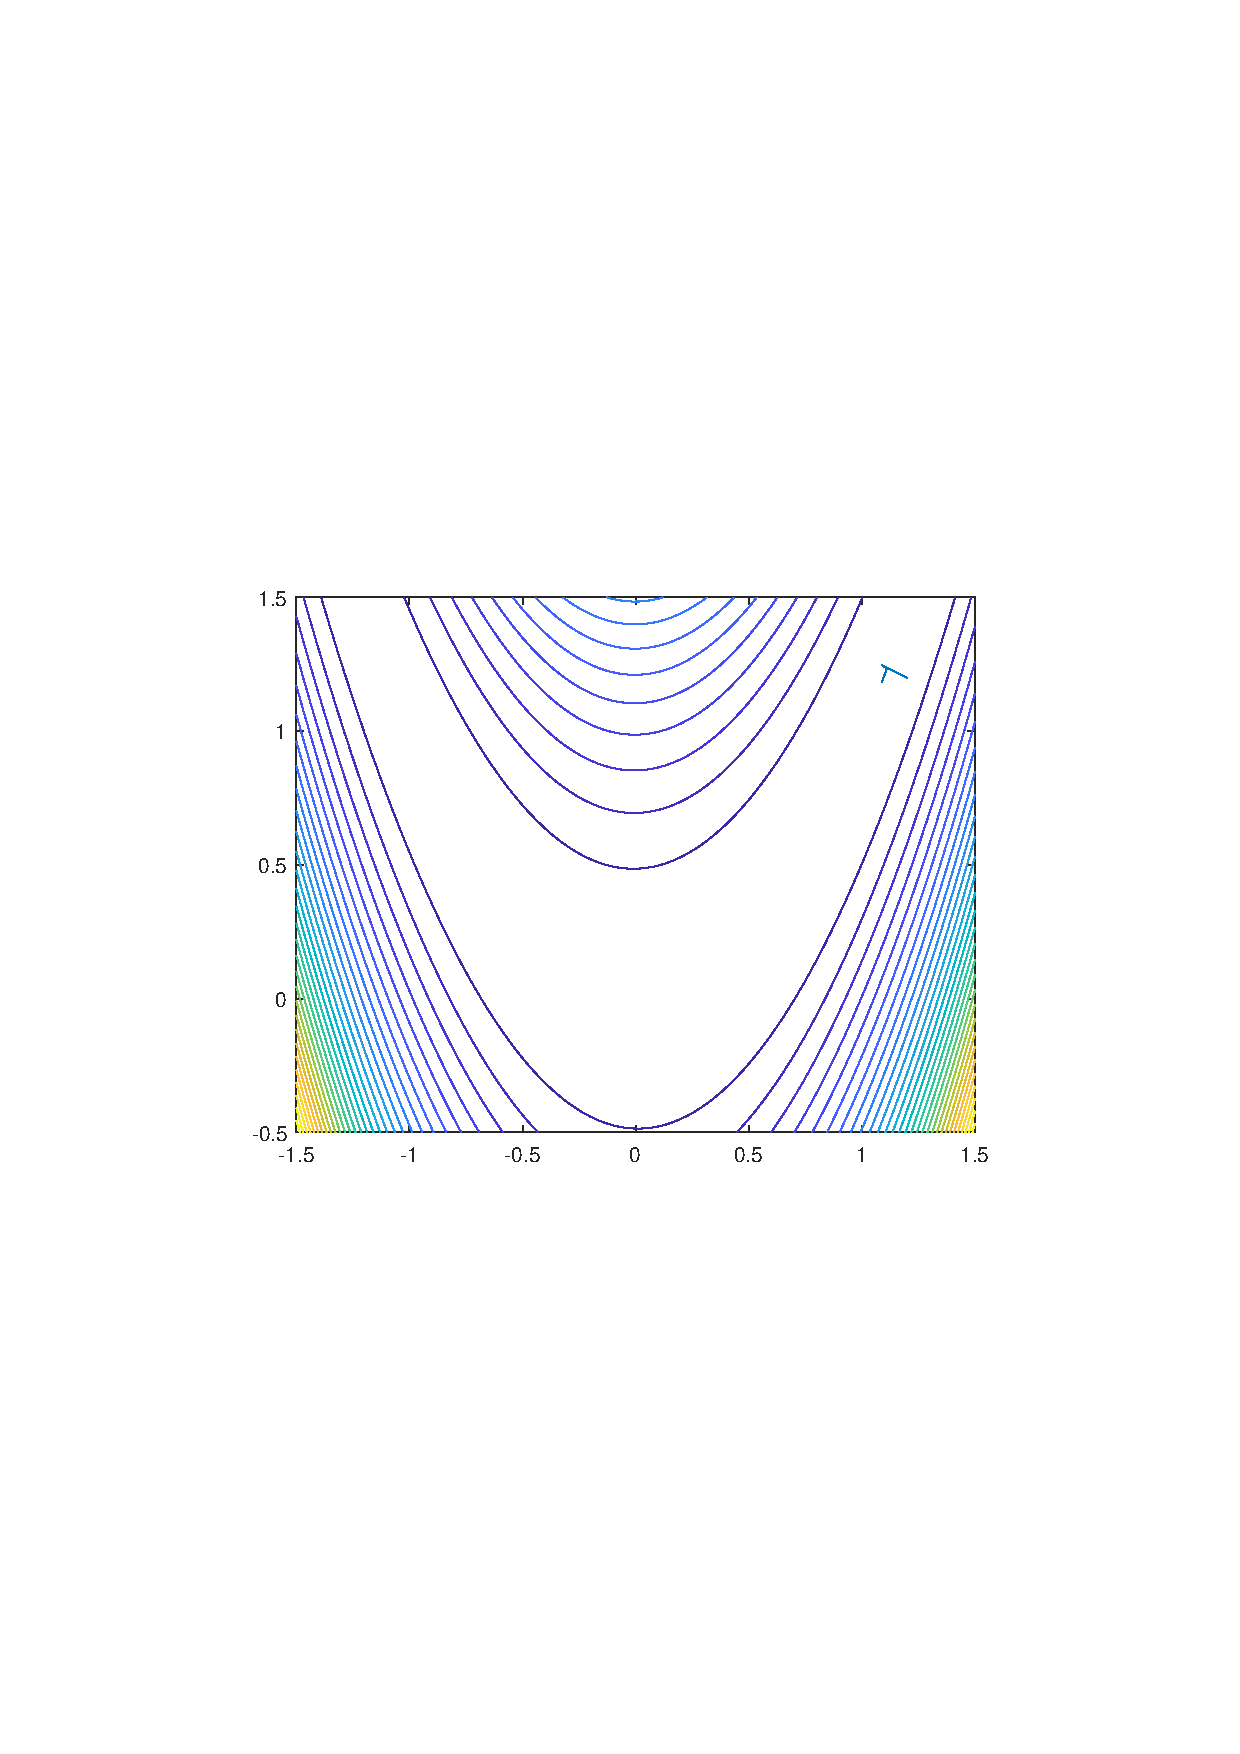
\includegraphics[width=5cm]{fig/4_11.pdf}}
\subfigure{
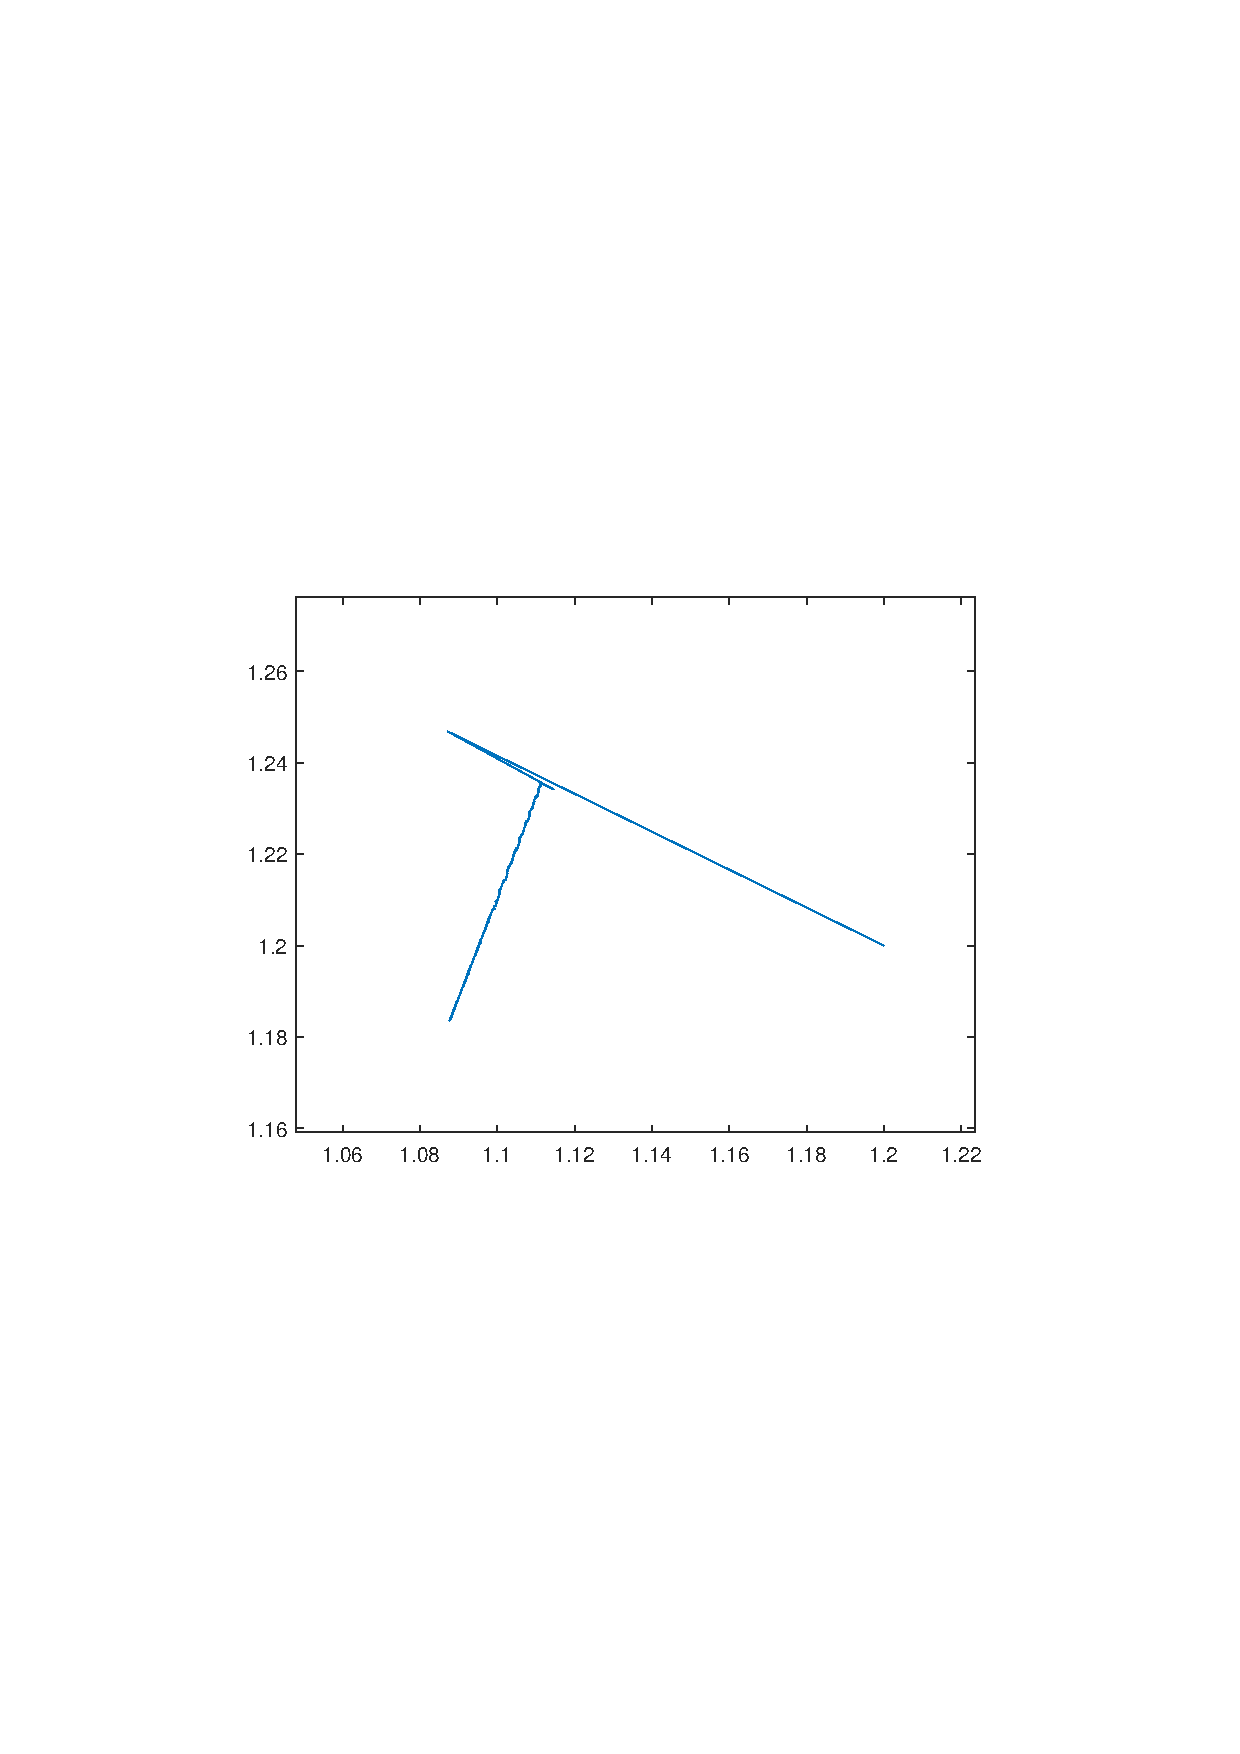
\includegraphics[width=5cm]{fig/4_12.pdf}}
\subfigure{
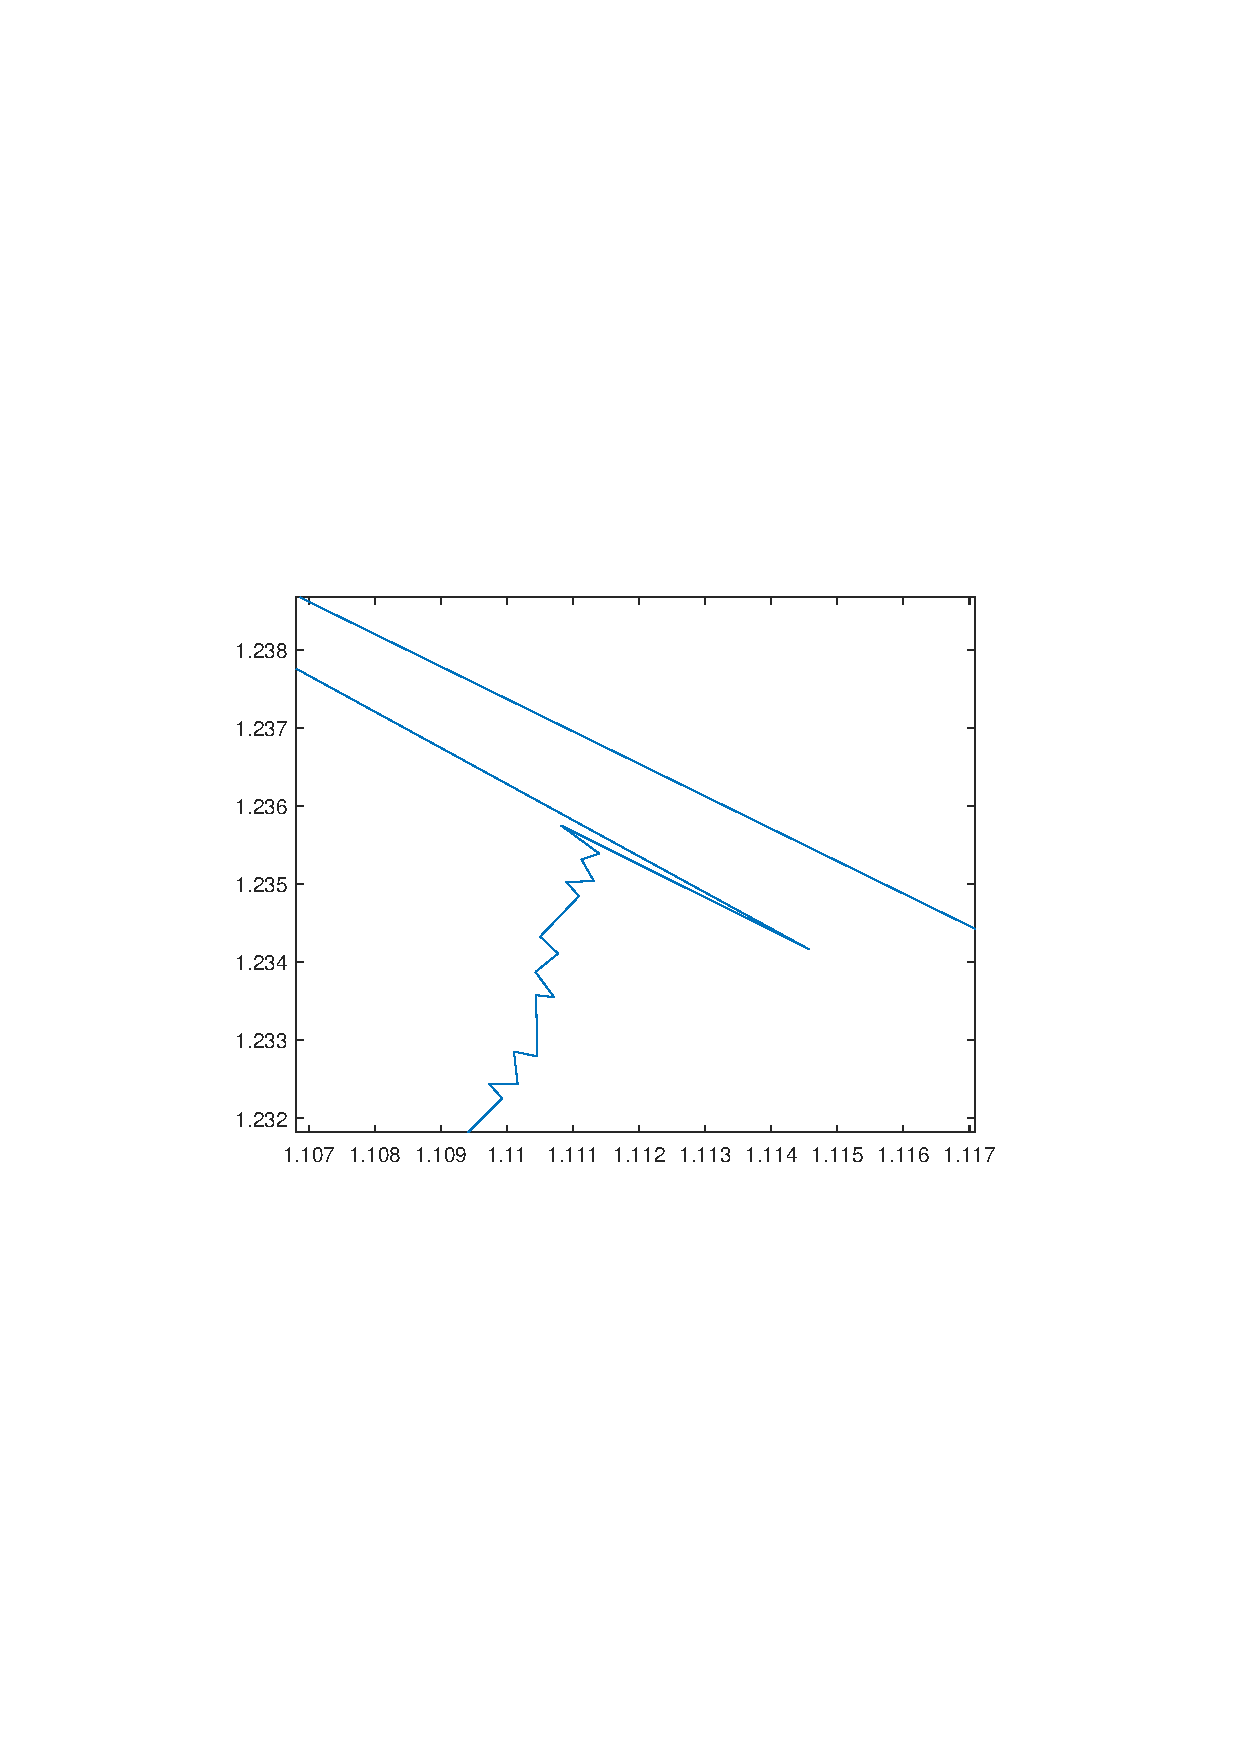
\includegraphics[width=5cm]{fig/4_13.pdf}}
\subfigure{
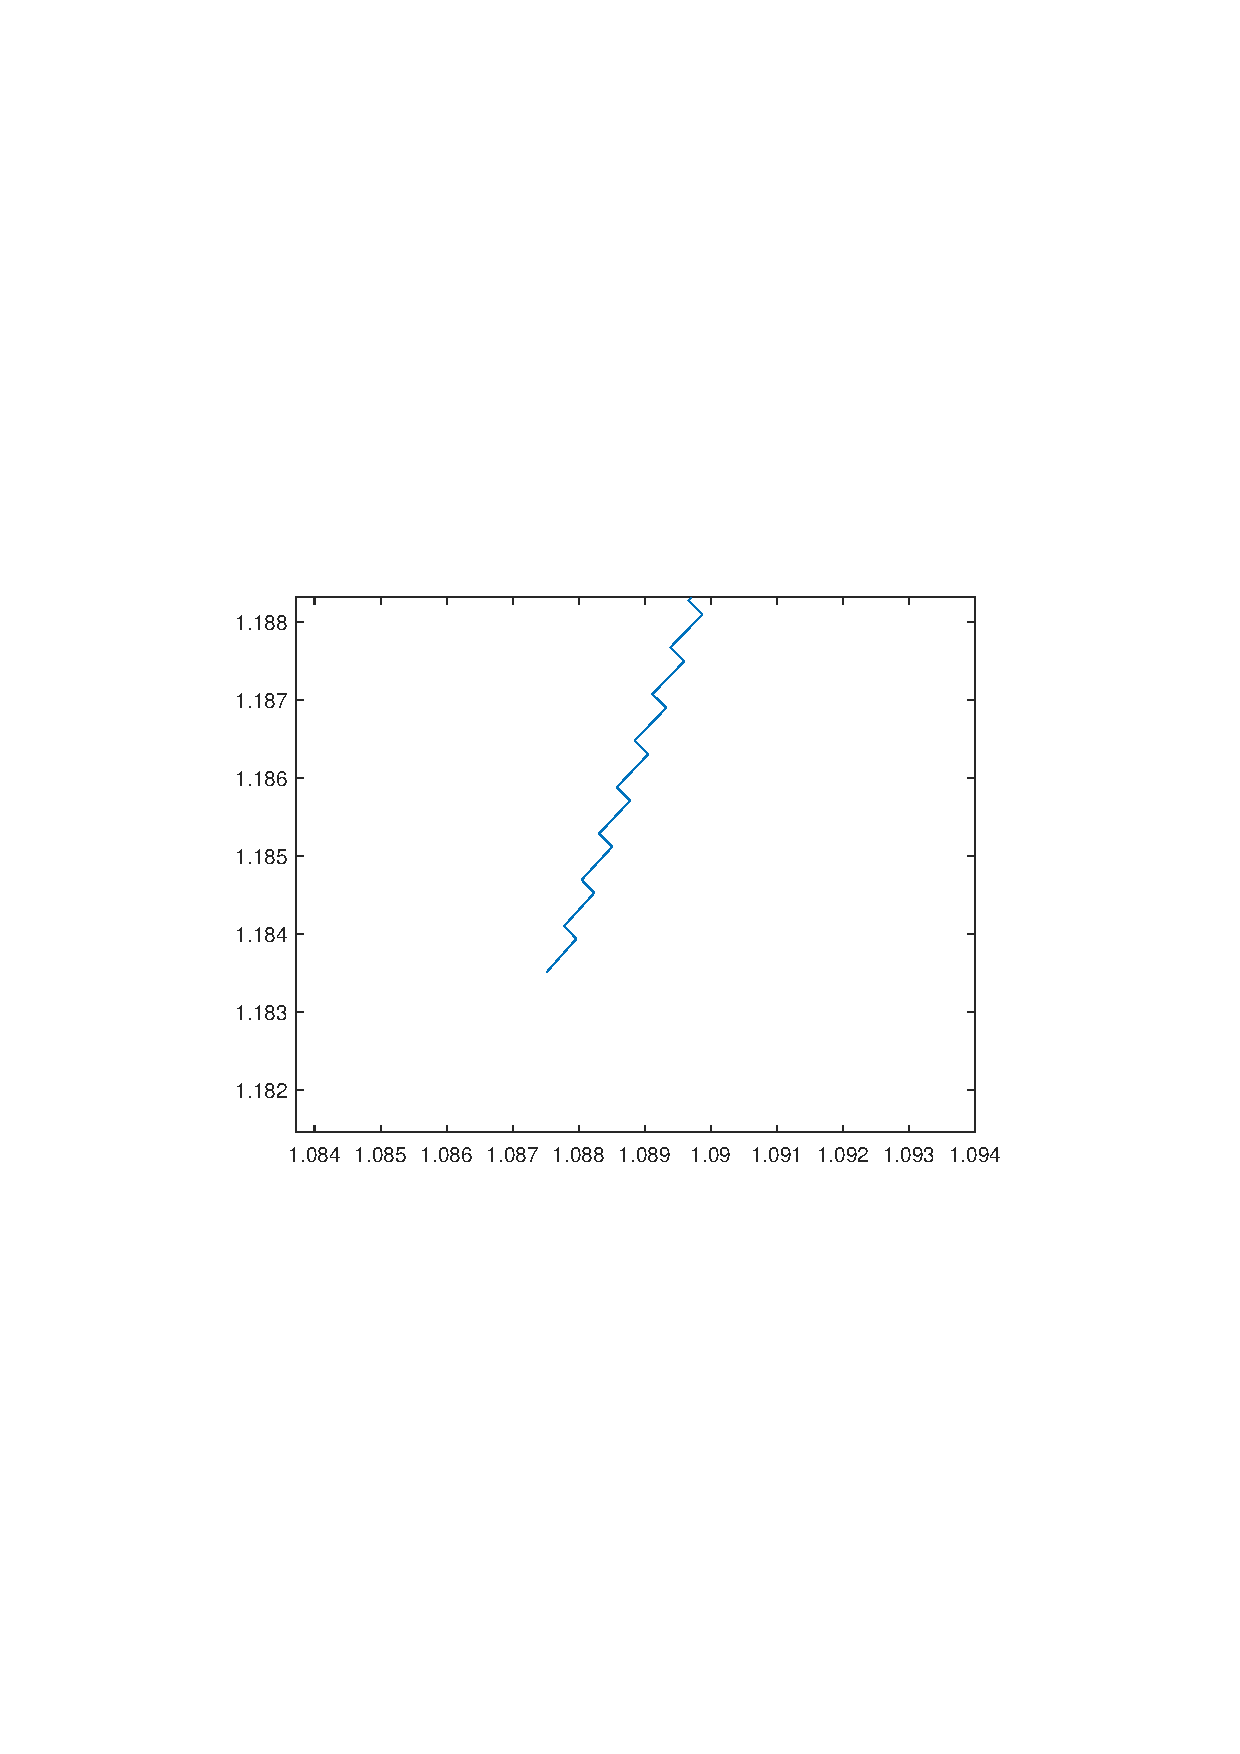
\includegraphics[width=5cm]{fig/4_14.pdf}}
\caption{Steepest-denscent in (1.2,1.2)}
\label{Fig.lable}
\end{figure}

\begin{figure}[H]
\centering
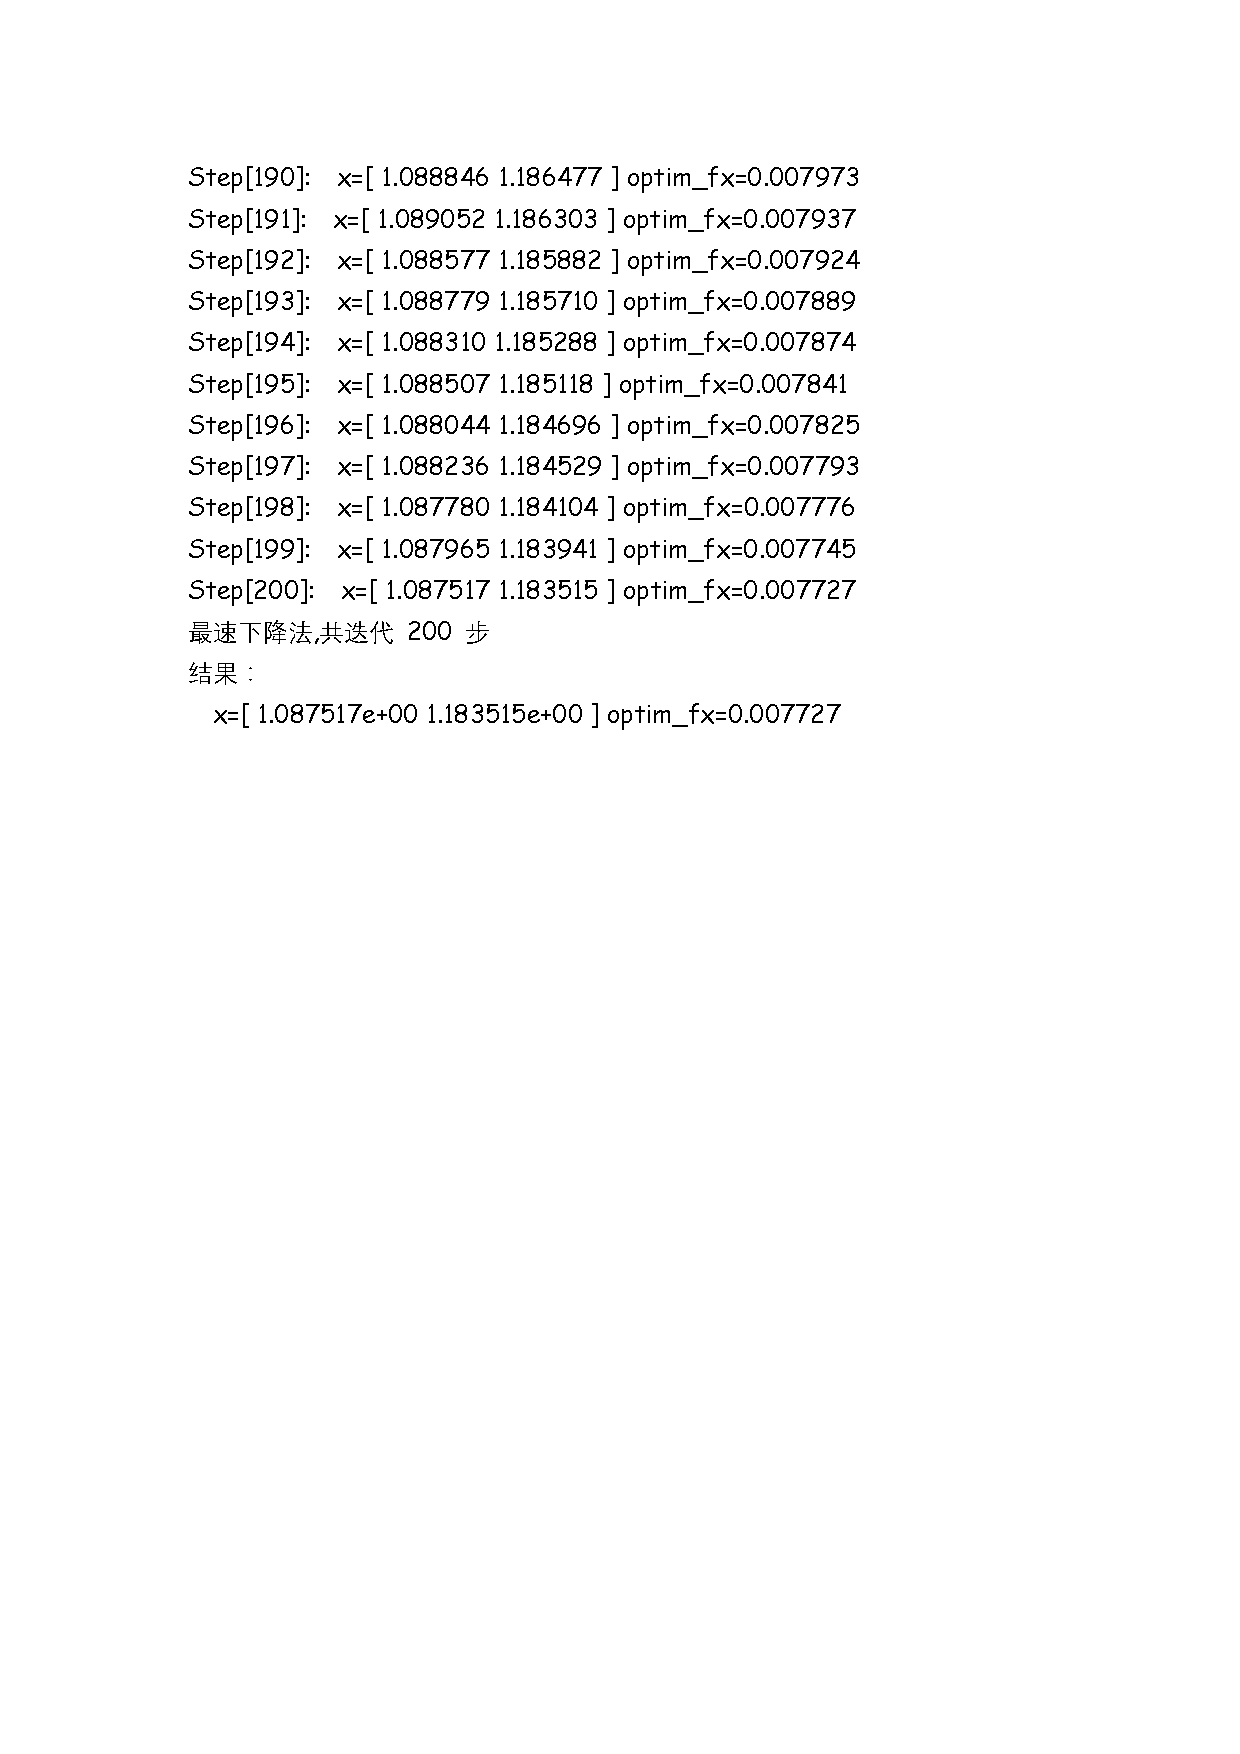
\includegraphics[width=10cm]{fig/4_15.pdf}
%\caption{在$(1,1)$处附近的三维等高线}
\end{figure}

\begin{figure}[H]
\centering
\subfigure{
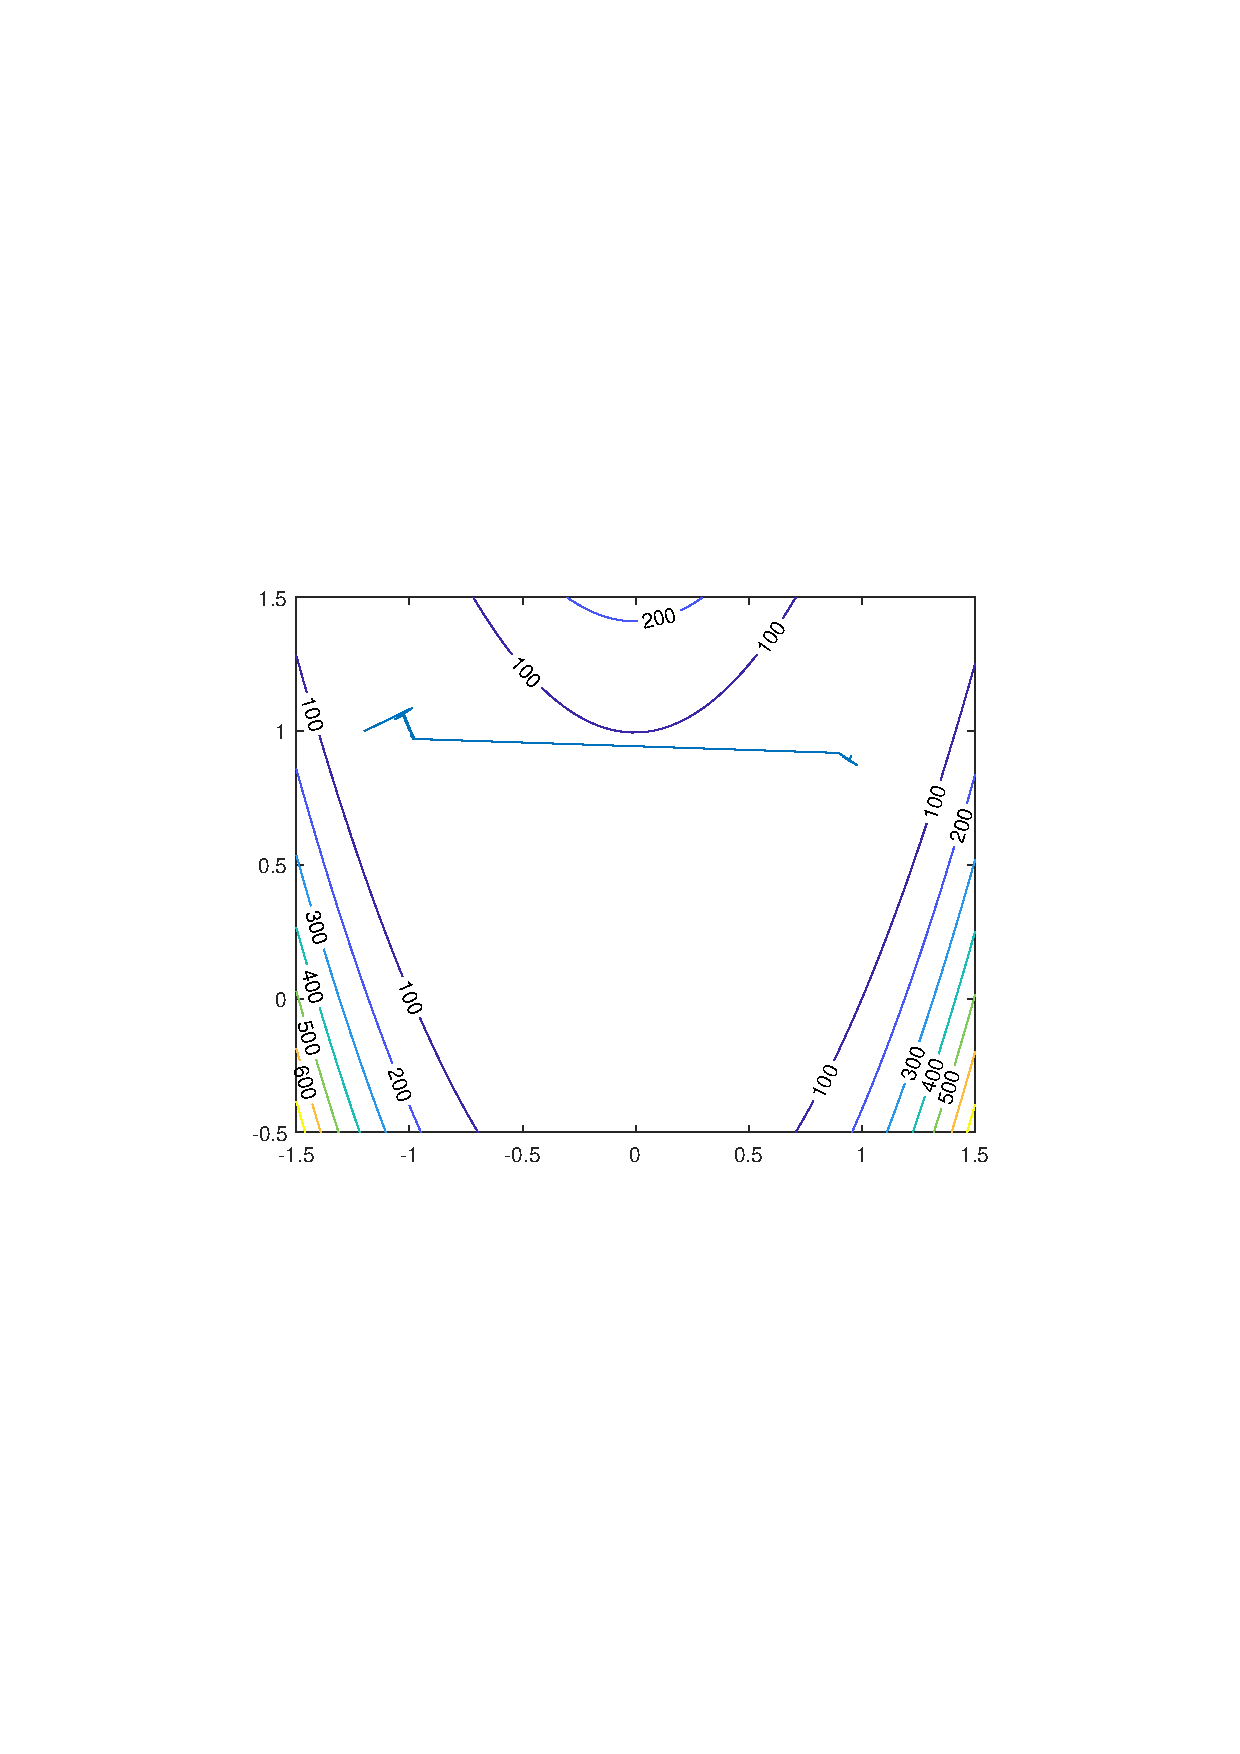
\includegraphics[width=5cm]{fig/4_21.pdf}}
\subfigure{
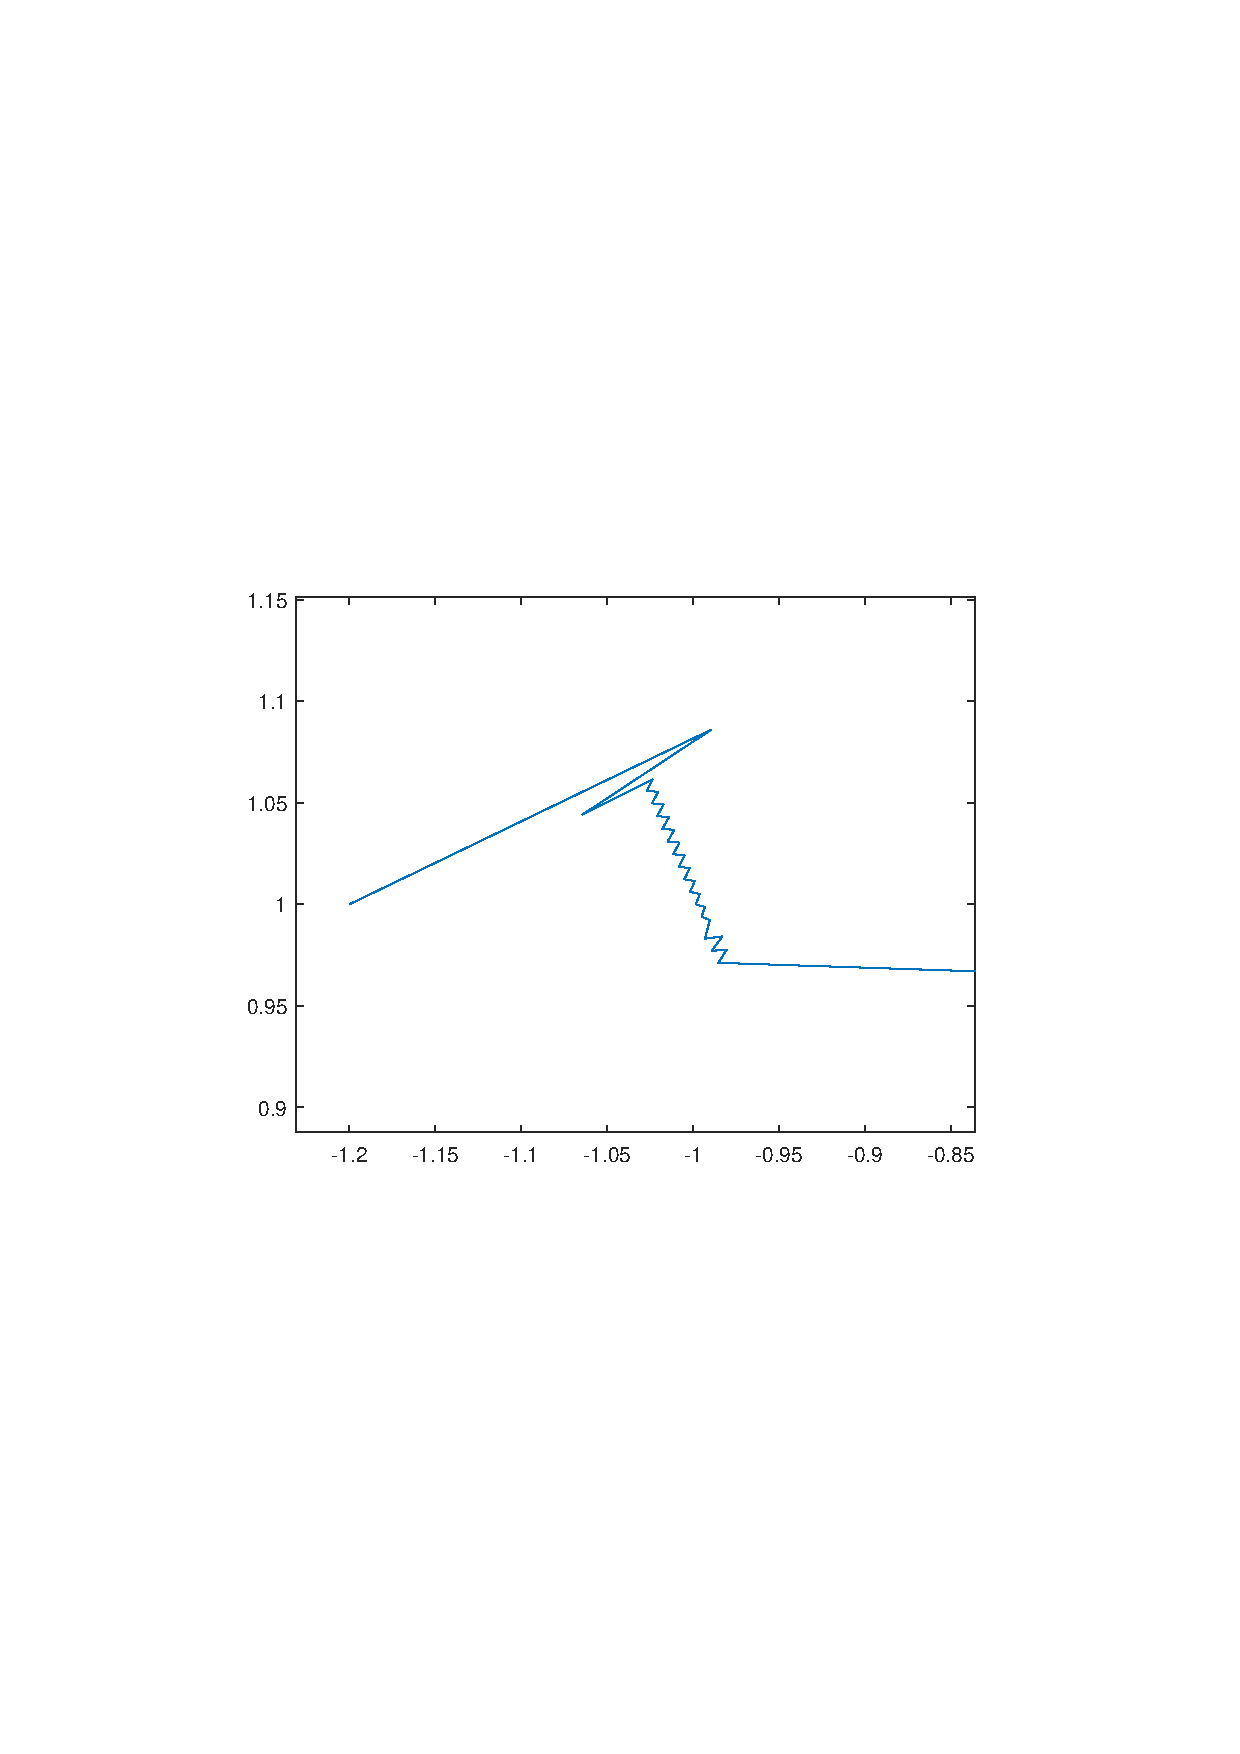
\includegraphics[width=5cm]{fig/4_22.pdf}}
\subfigure{
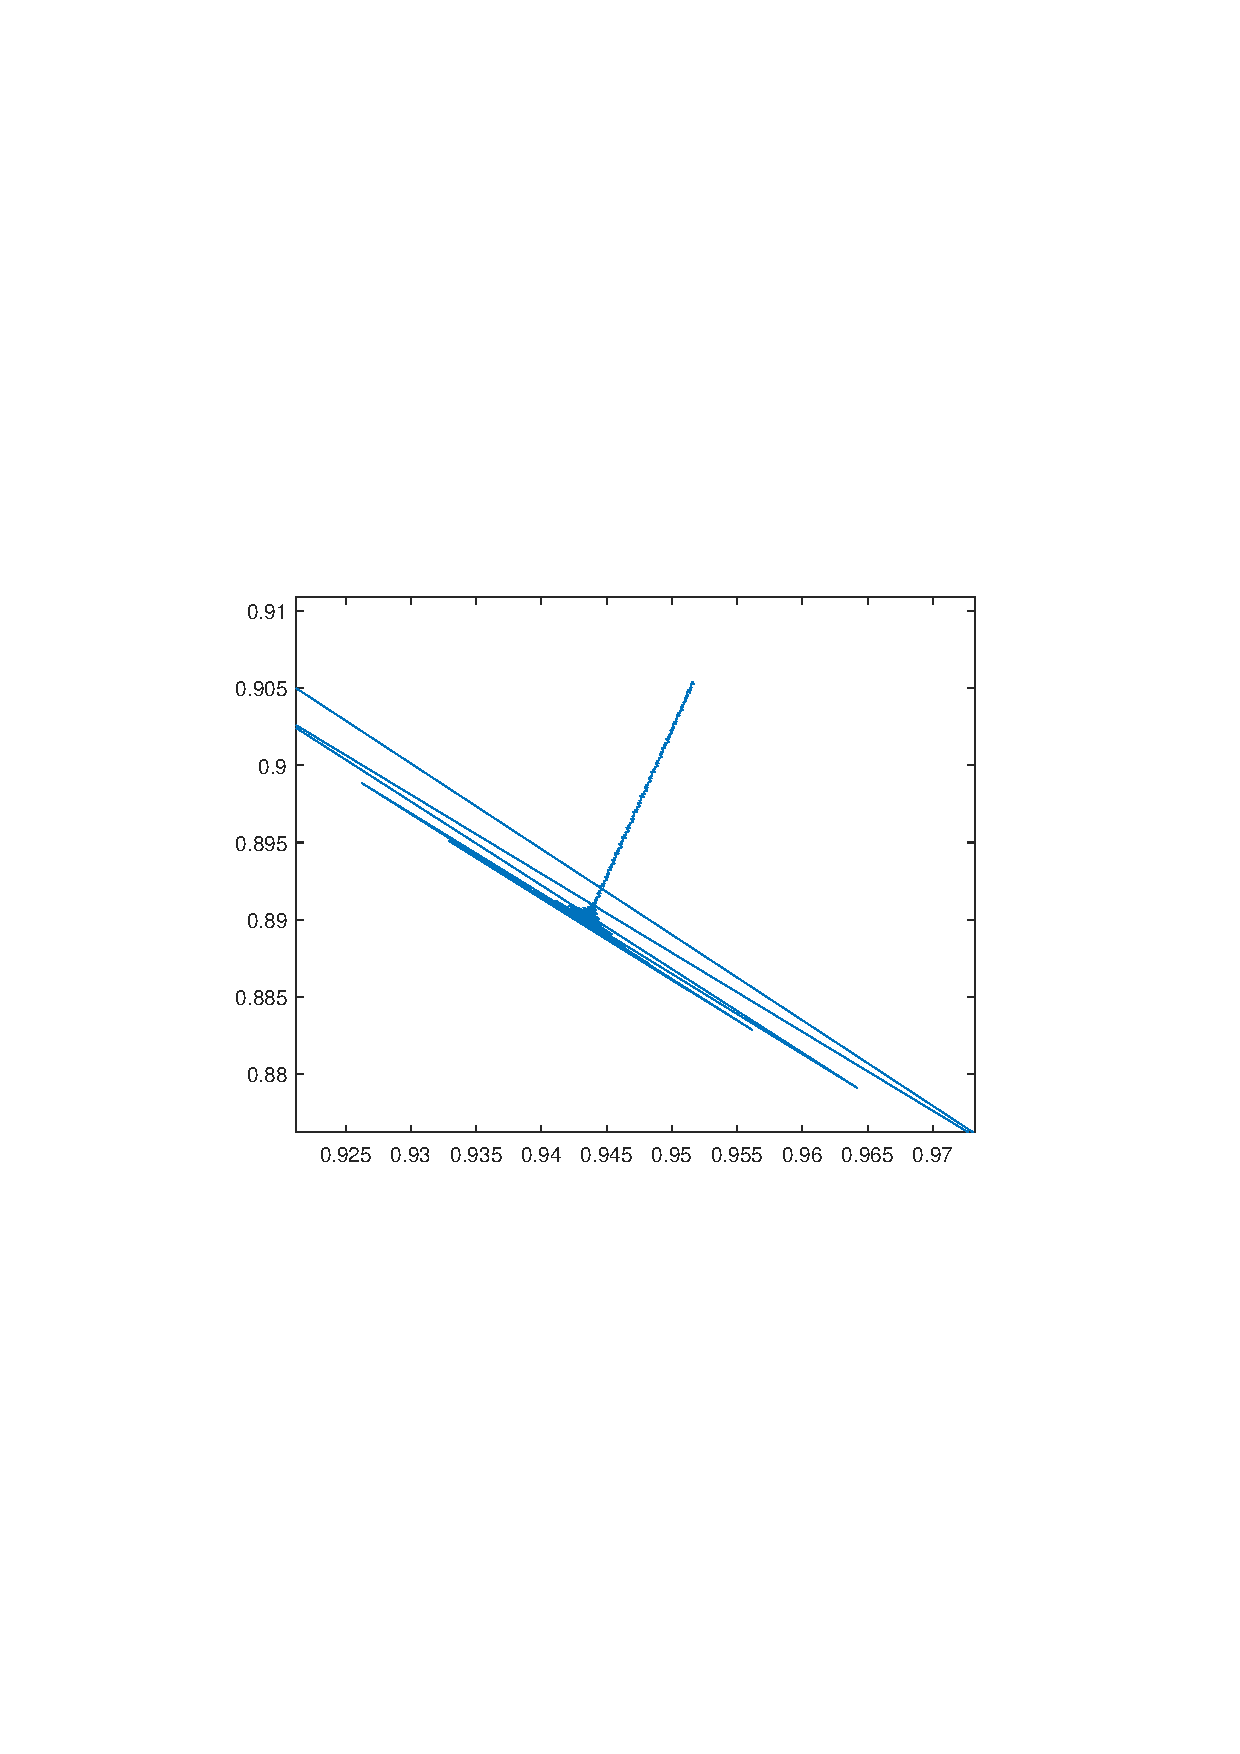
\includegraphics[width=5cm]{fig/4_23.pdf}}
\subfigure{
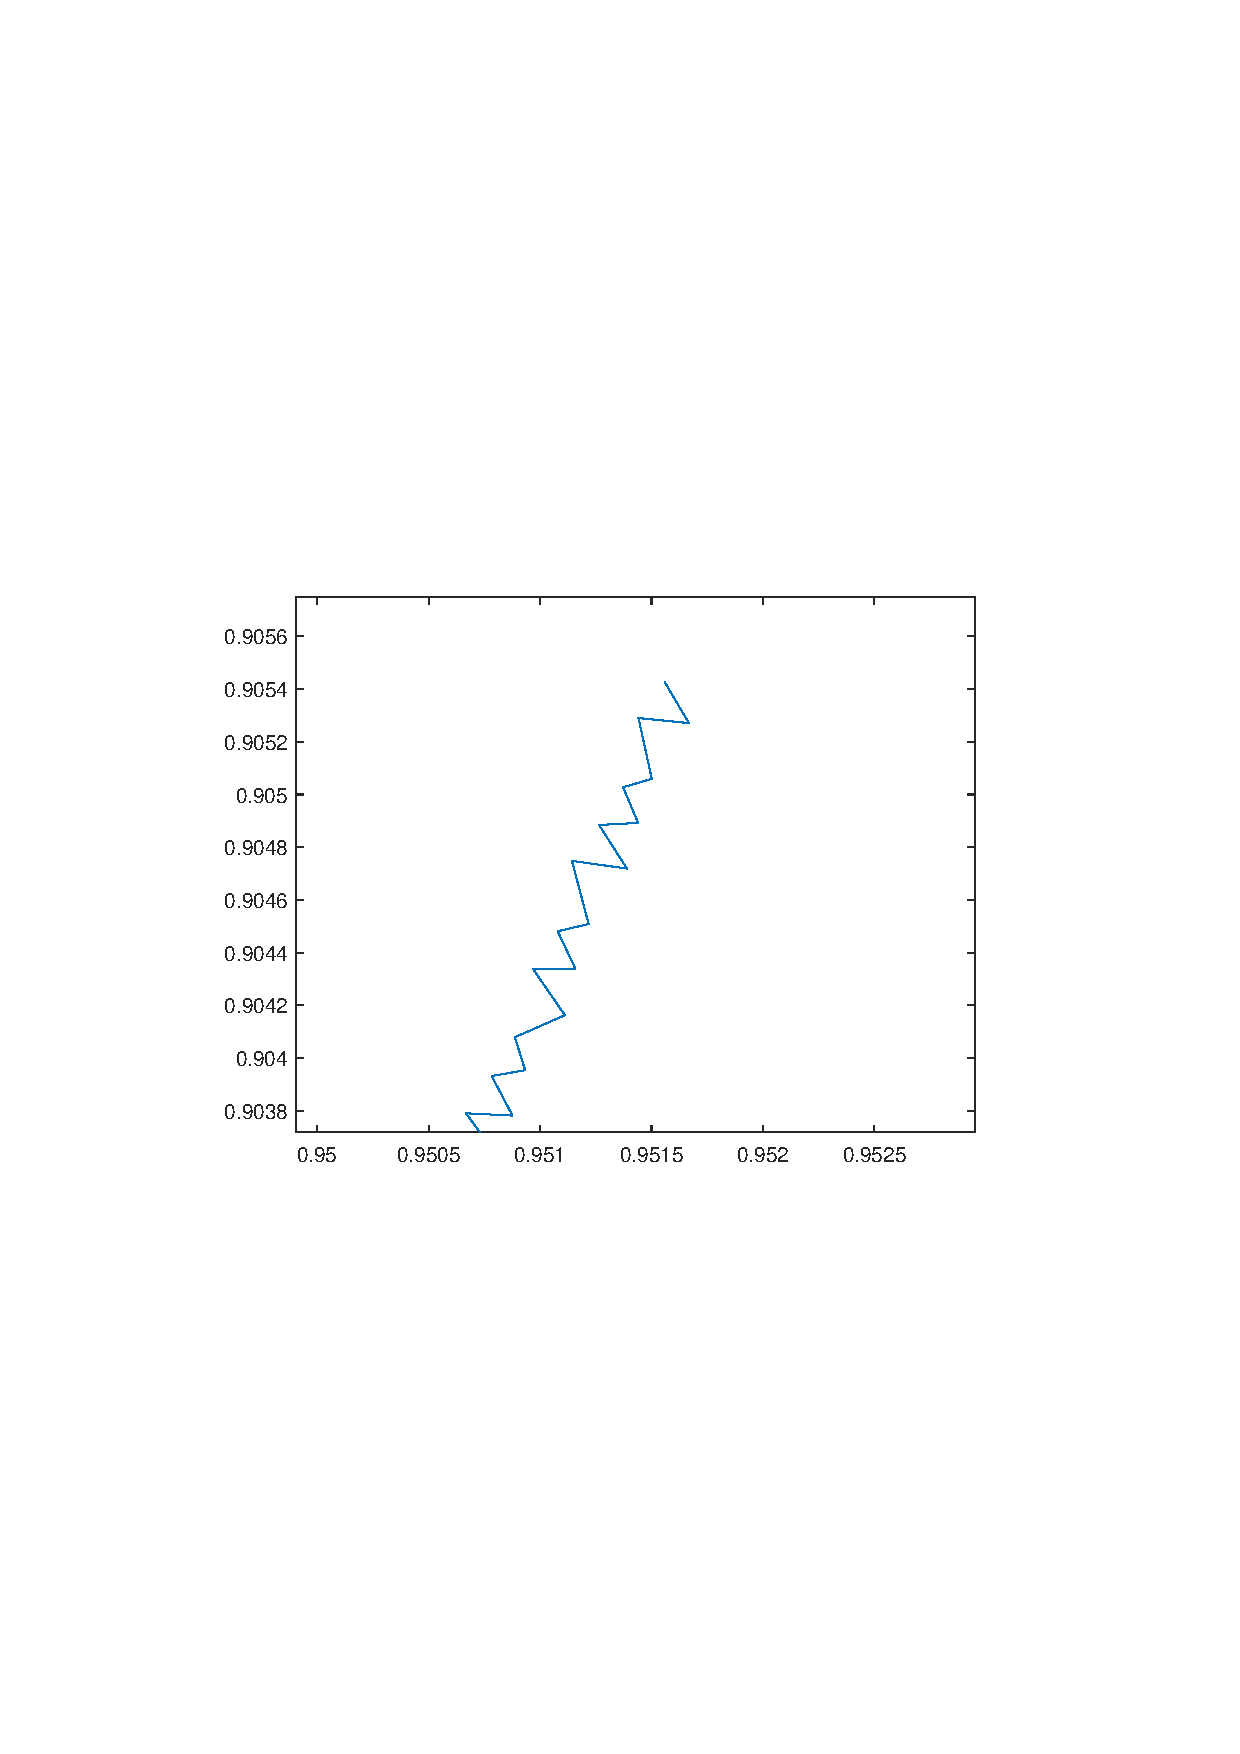
\includegraphics[width=5cm]{fig/4_24.pdf}}
\caption{Steepest-denscent in (-1.2,1)}
\label{Fig.lable}
\end{figure}

\begin{figure}[H]
\centering
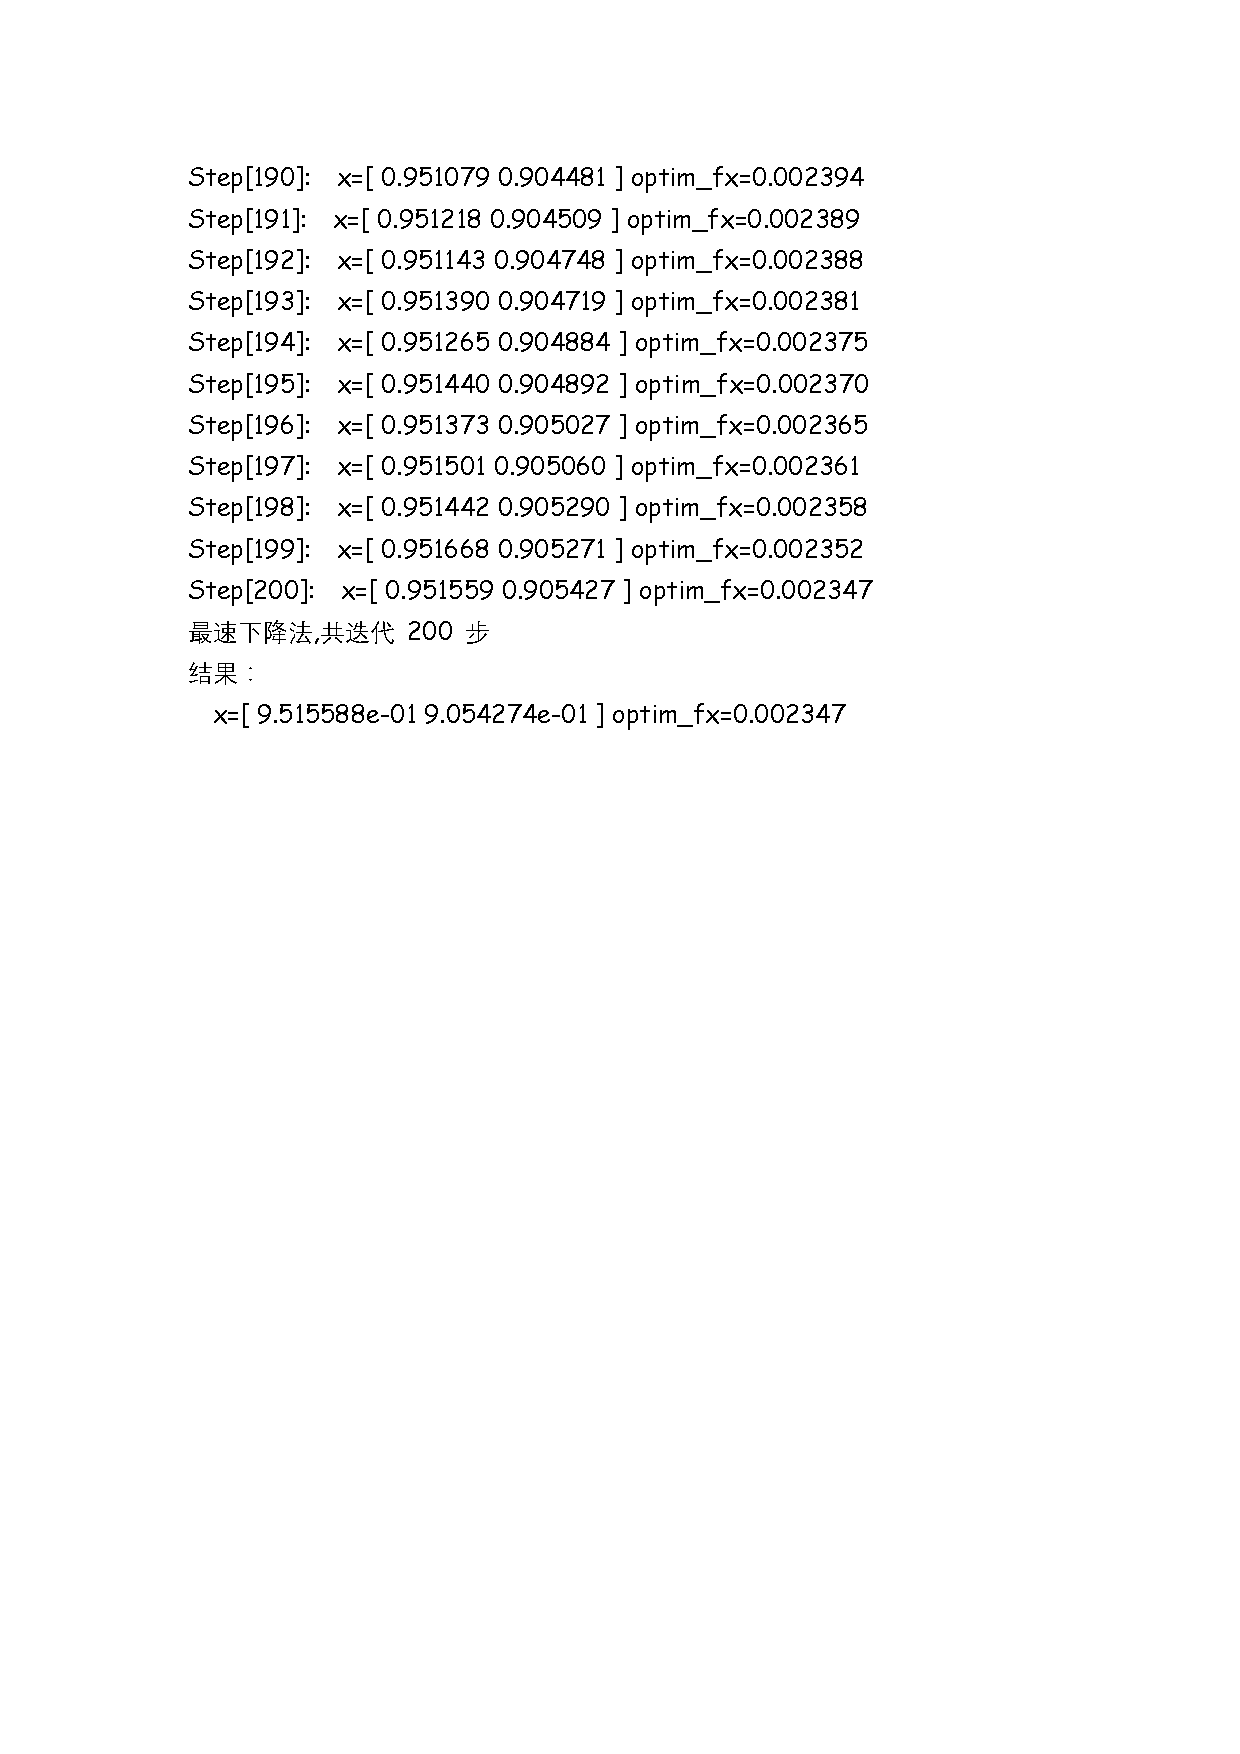
\includegraphics[width=10cm]{fig/4_25.pdf}
%\caption{在$(1,1)$处附近的三维等高线}
\end{figure}

\begin{figure}[H]
\centering
\subfigure{
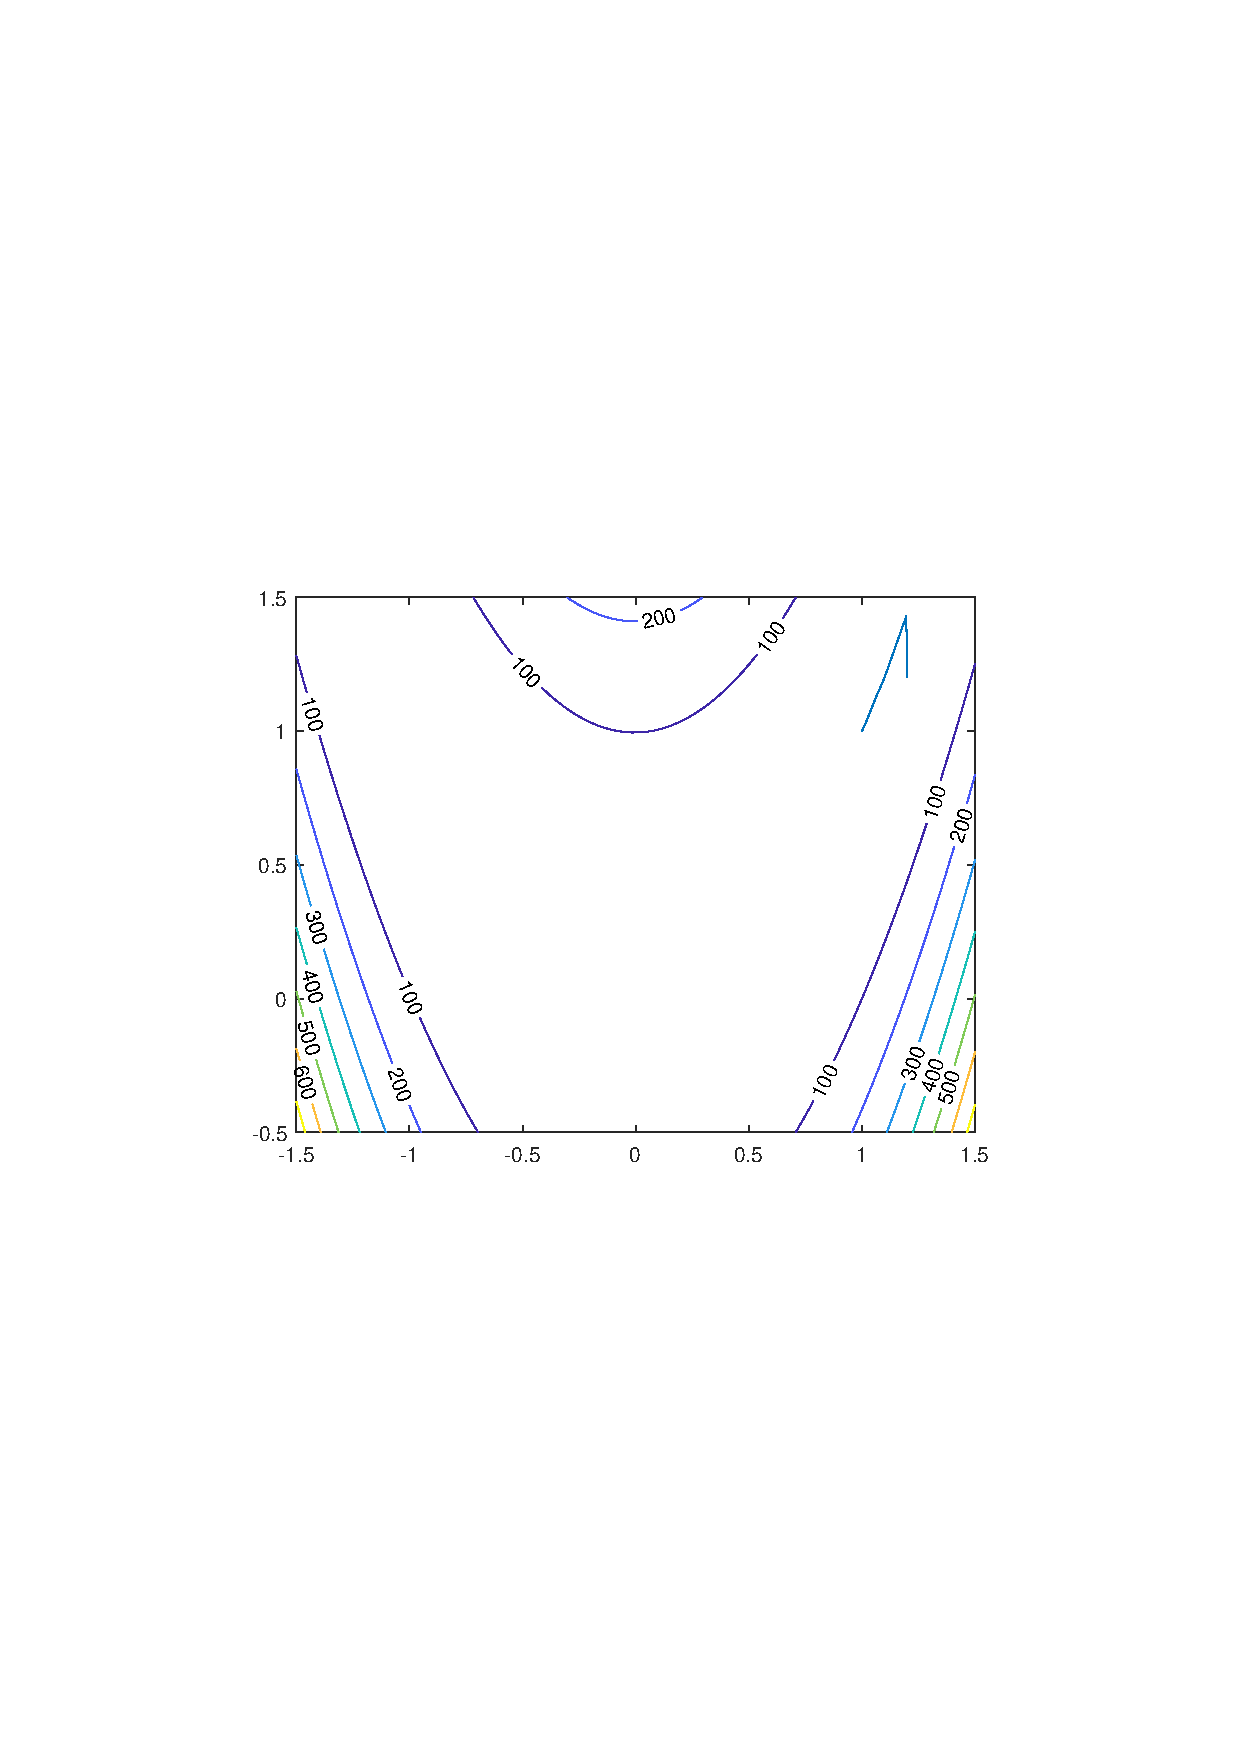
\includegraphics[width=5cm]{fig/4_31.pdf}}
\subfigure{
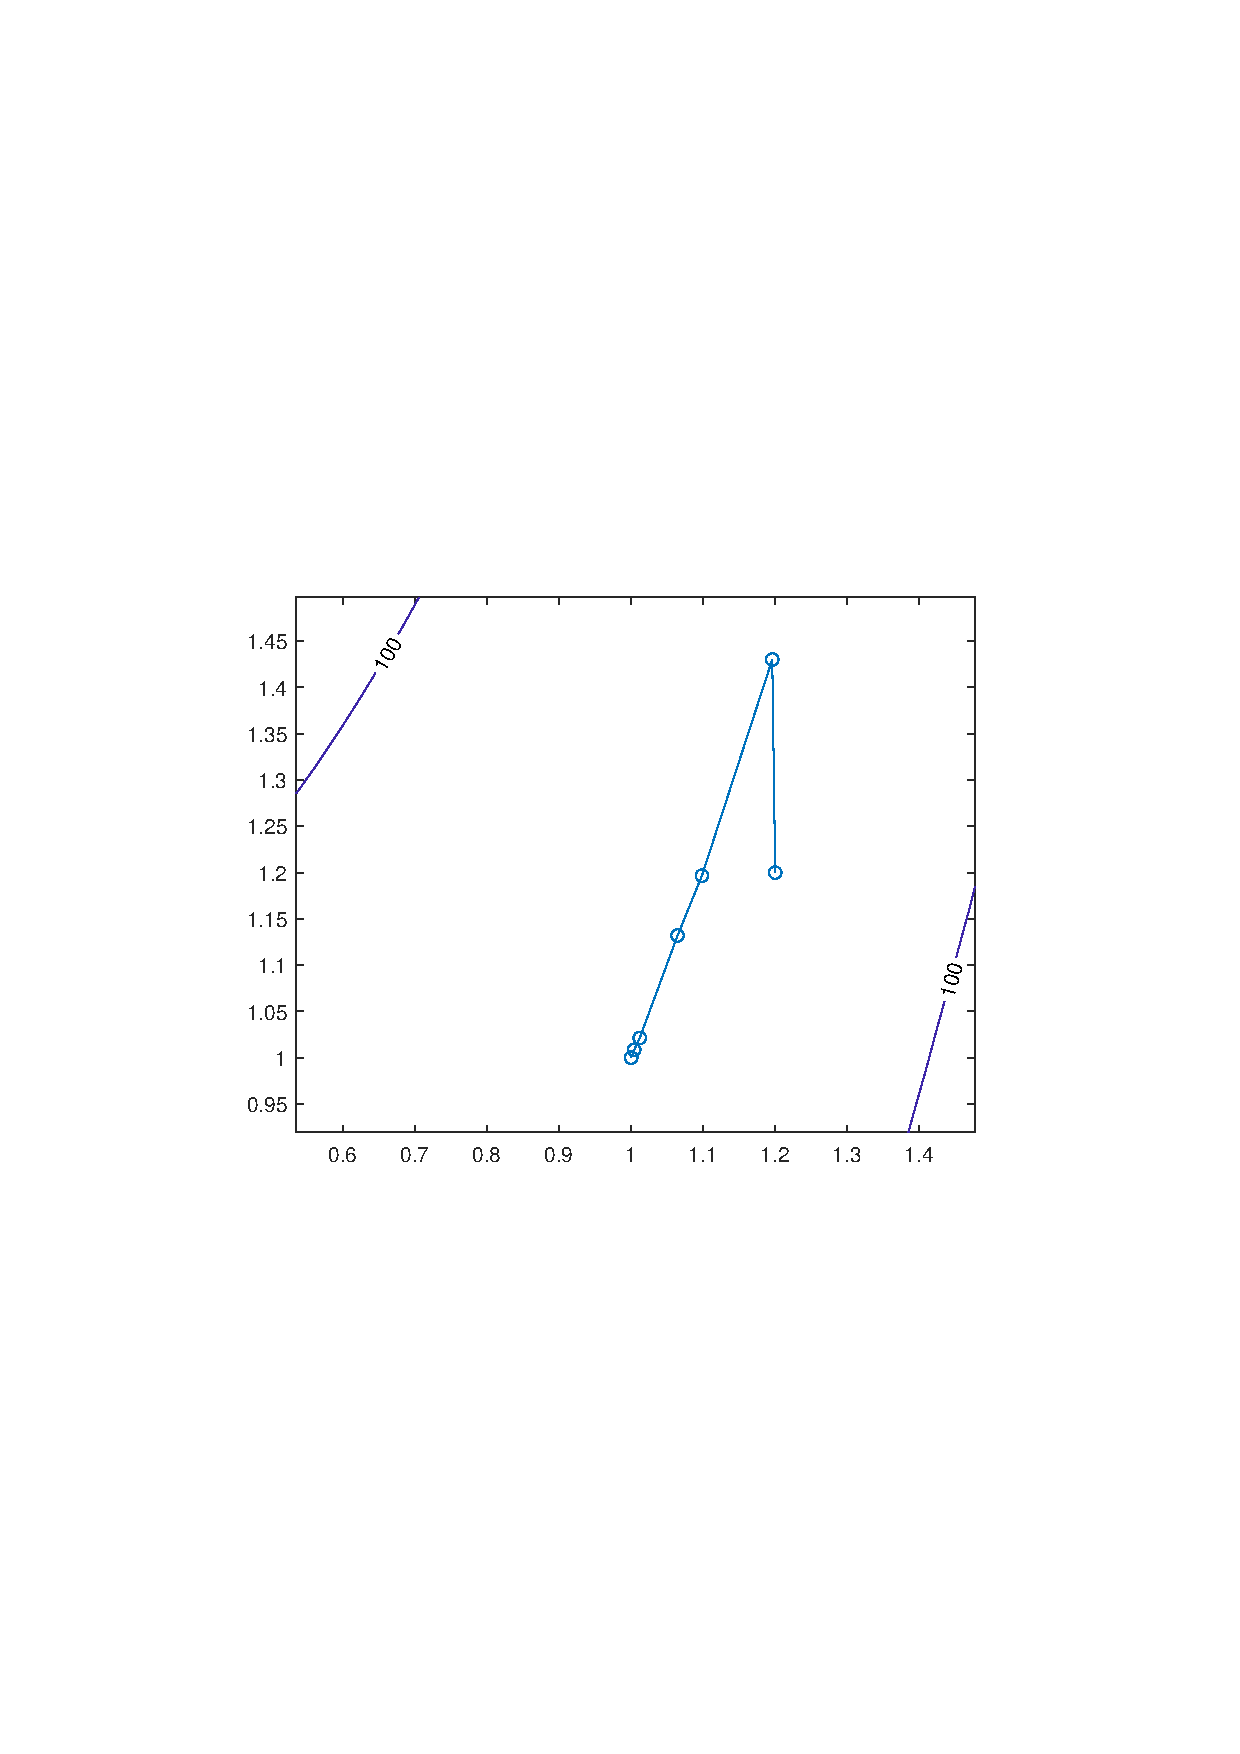
\includegraphics[width=5cm]{fig/4_32.pdf}}
\subfigure{
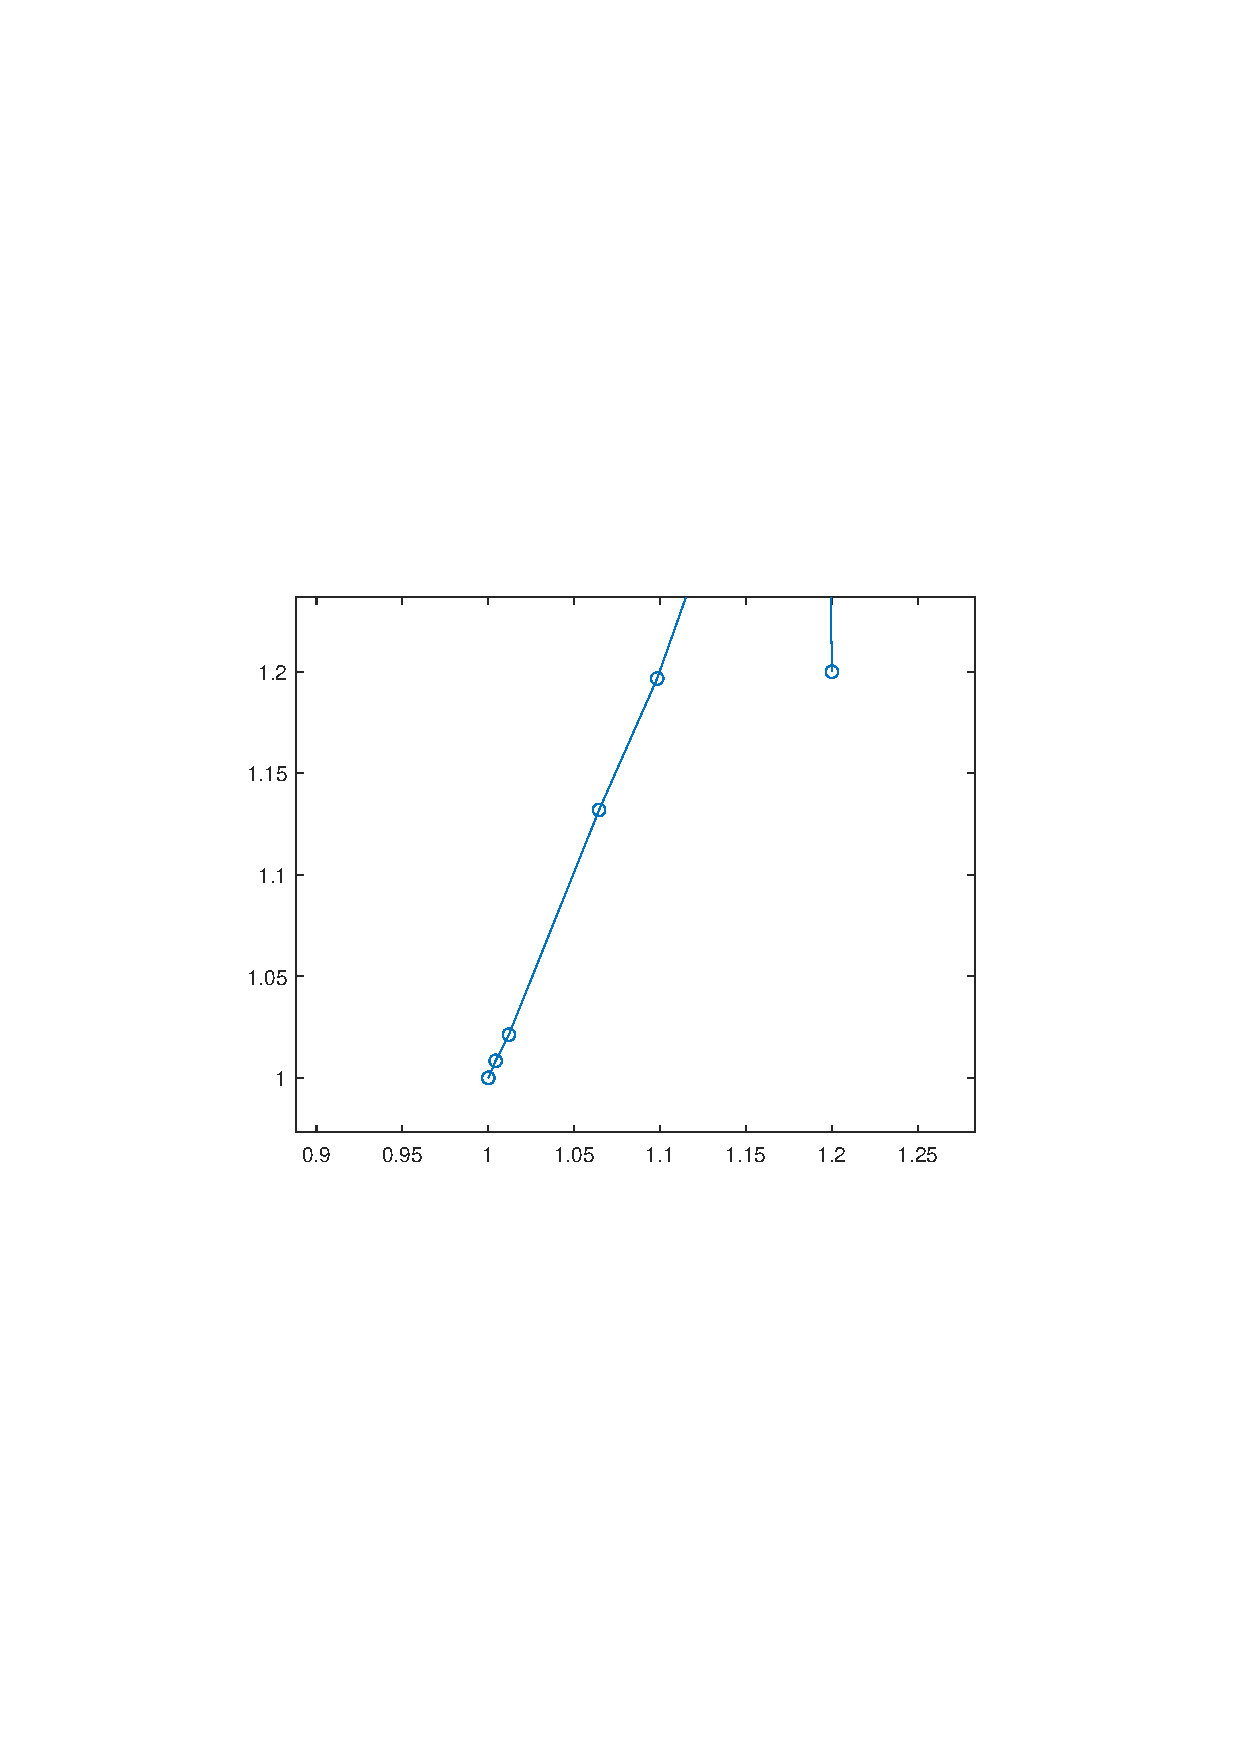
\includegraphics[width=5cm]{fig/4_33.pdf}}
\subfigure{
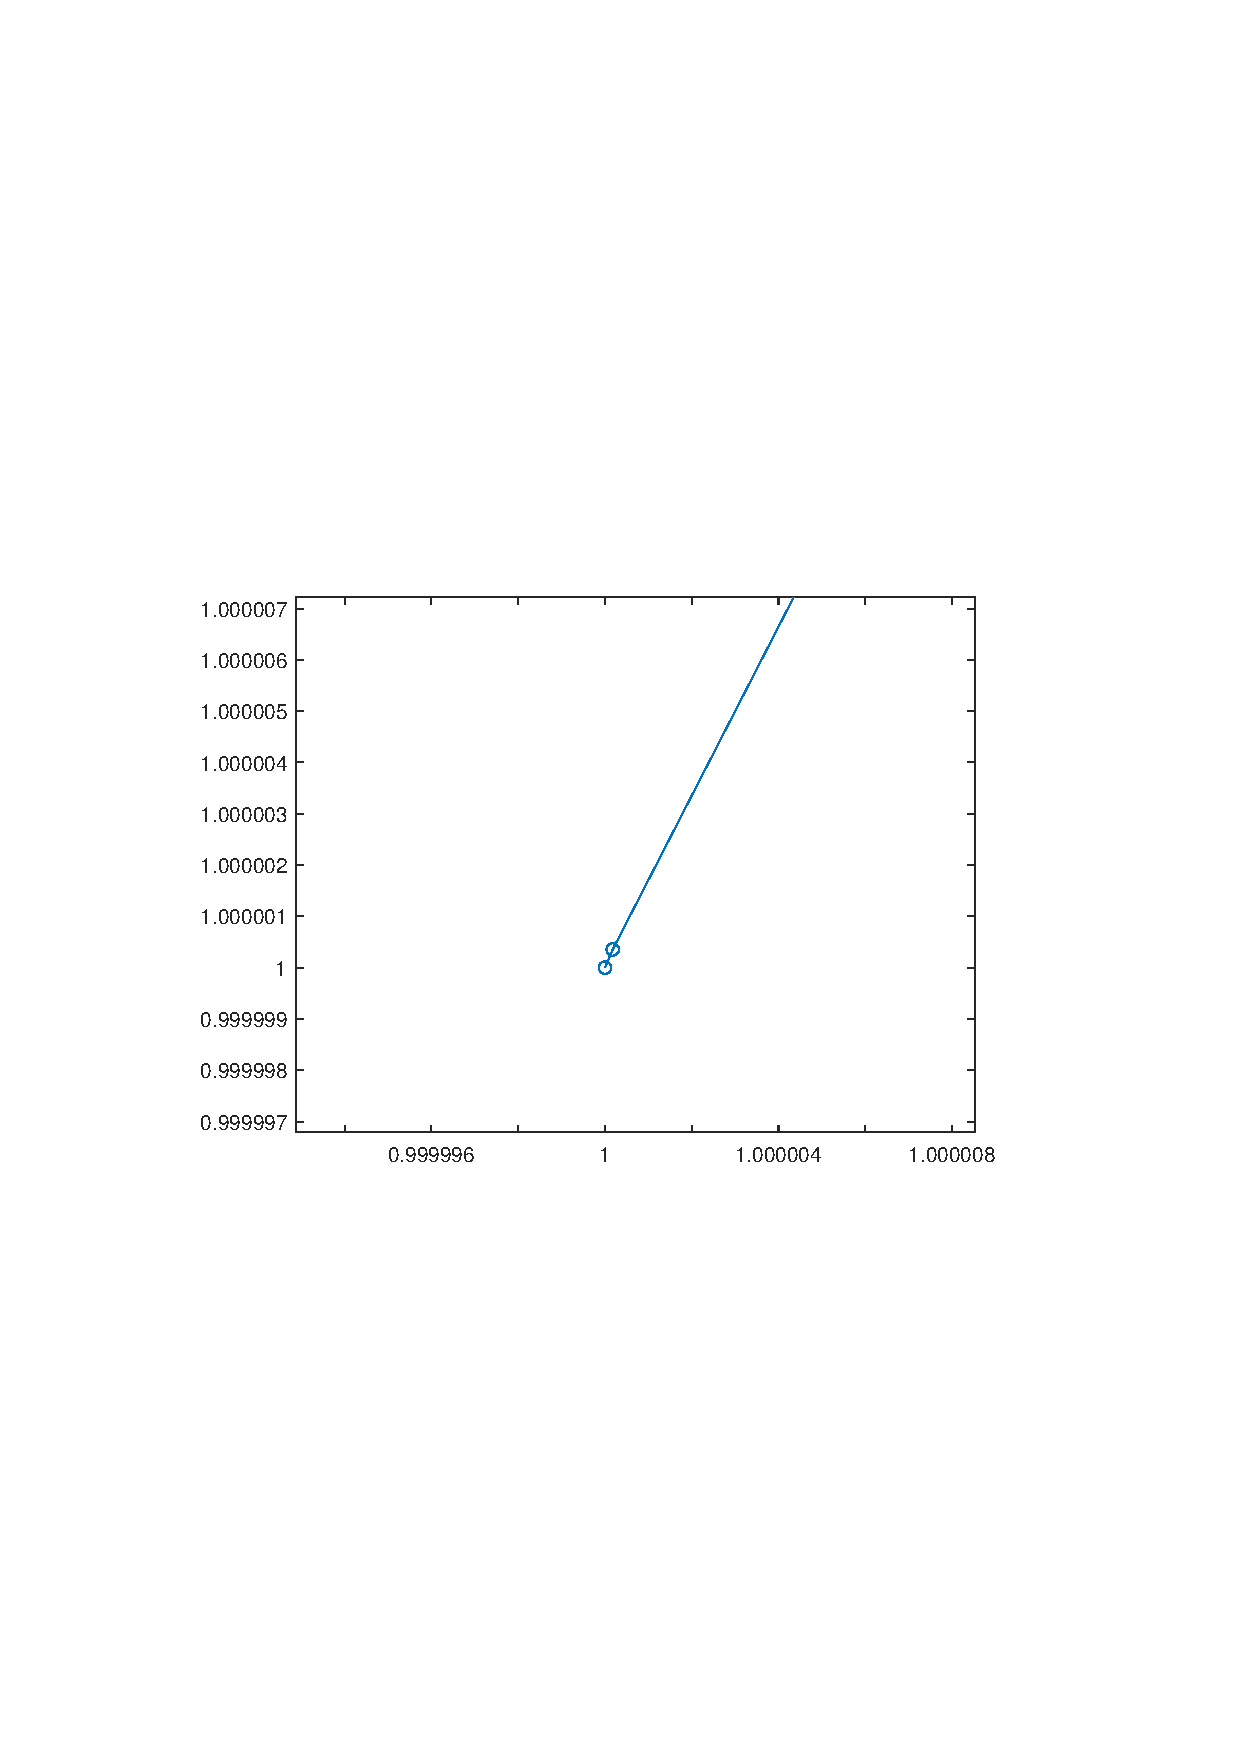
\includegraphics[width=5.3cm]{fig/4_34.pdf}}
\caption{Newton-Armijo in (1.2,1.2)}
\label{Fig.lable}
\end{figure}

\begin{figure}[H]
\centering
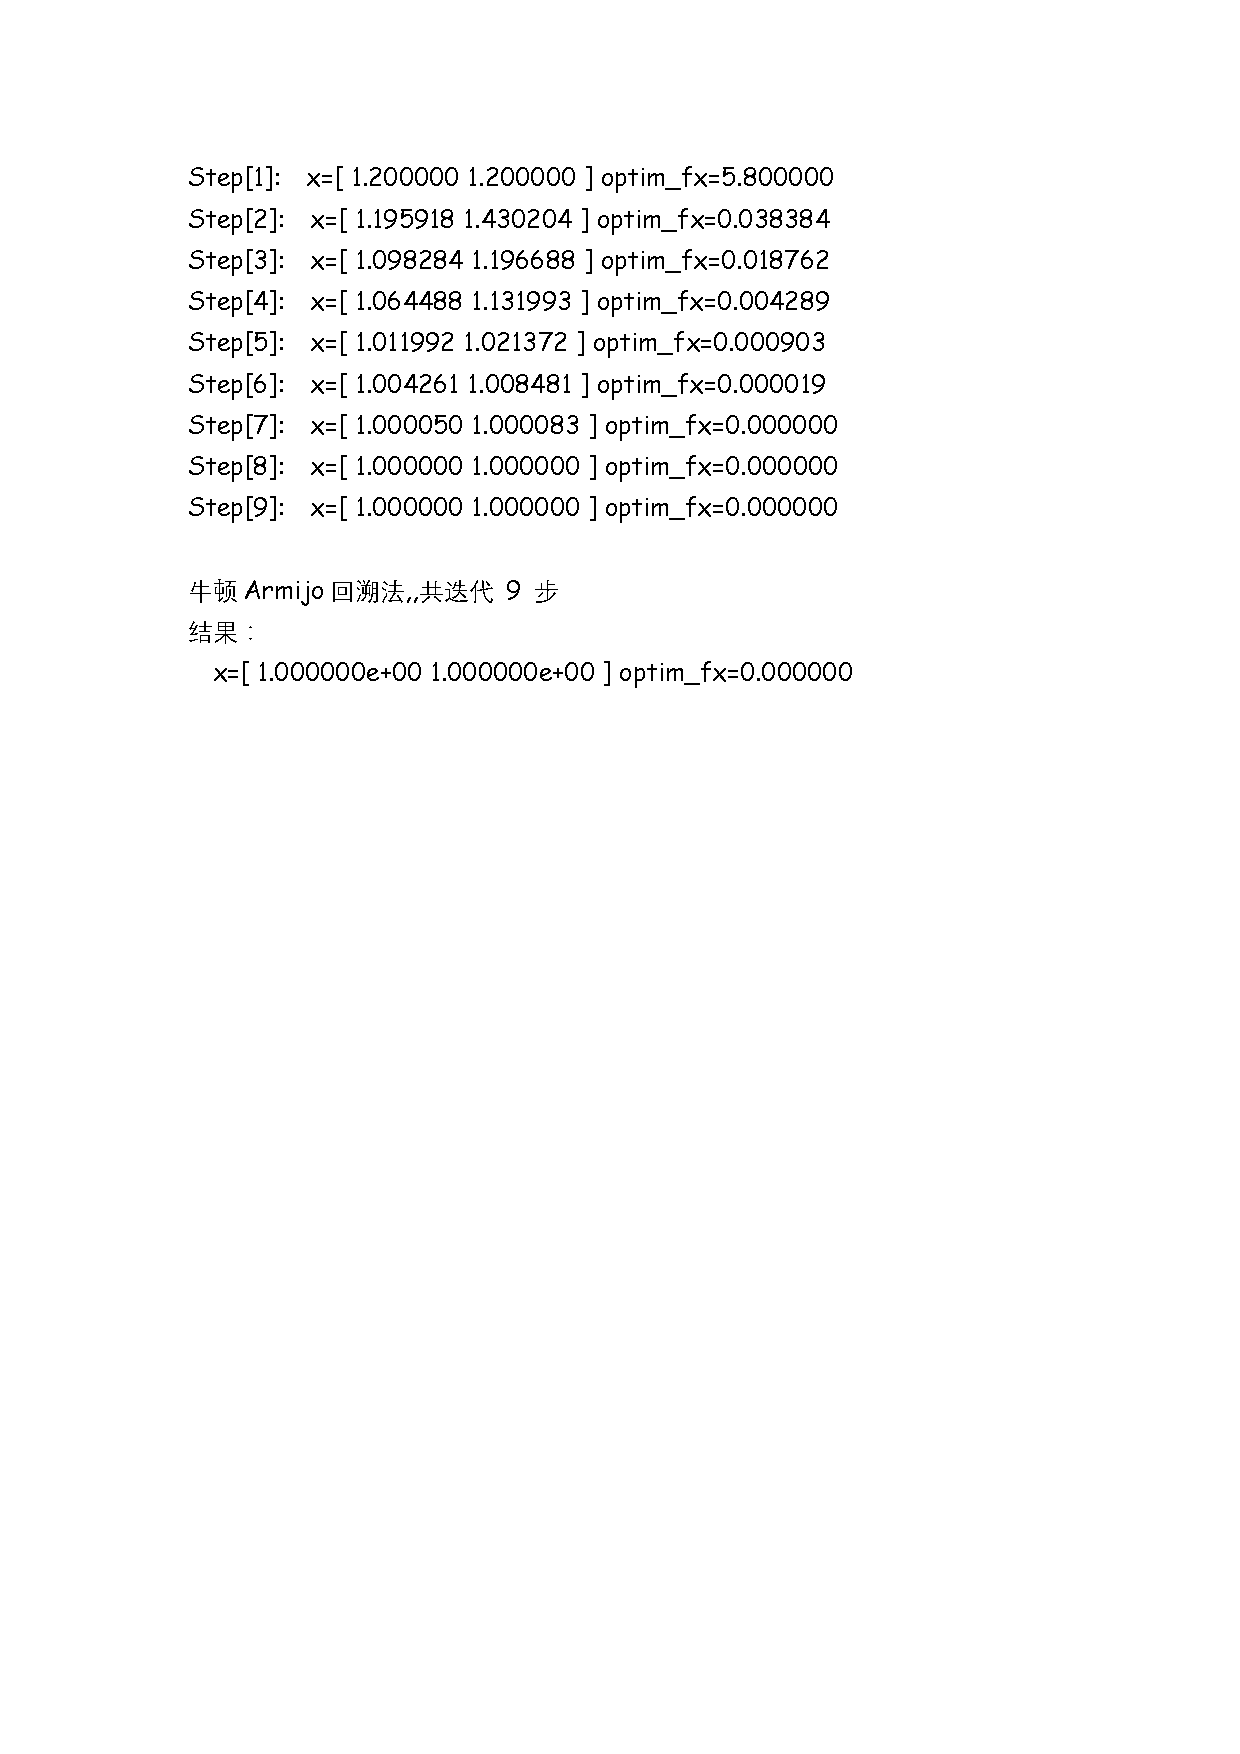
\includegraphics[width=10cm]{fig/4_35.pdf}
%\caption{在$(1,1)$处附近的三维等高线}
\end{figure}

\begin{figure}[H]
\centering
\subfigure{
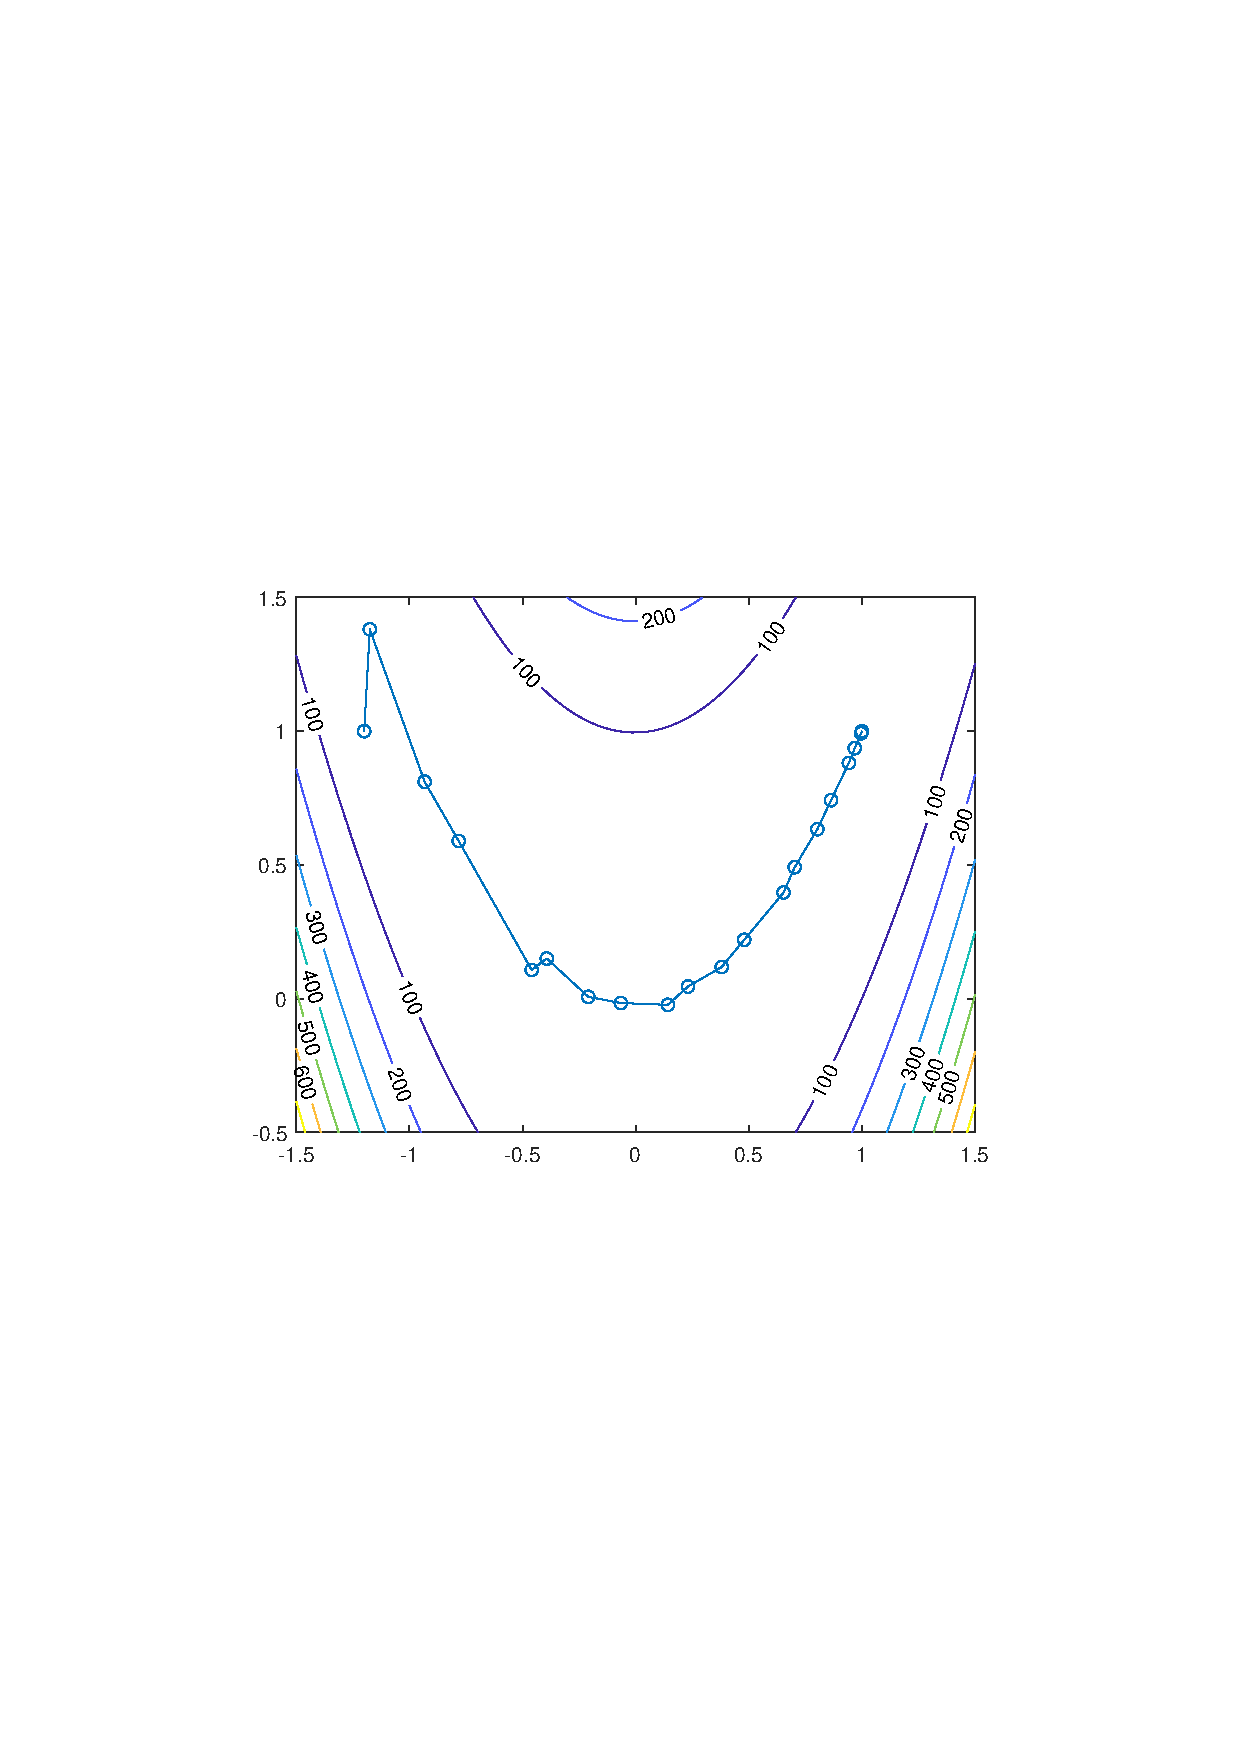
\includegraphics[width=5cm]{fig/4_41.pdf}}
\subfigure{
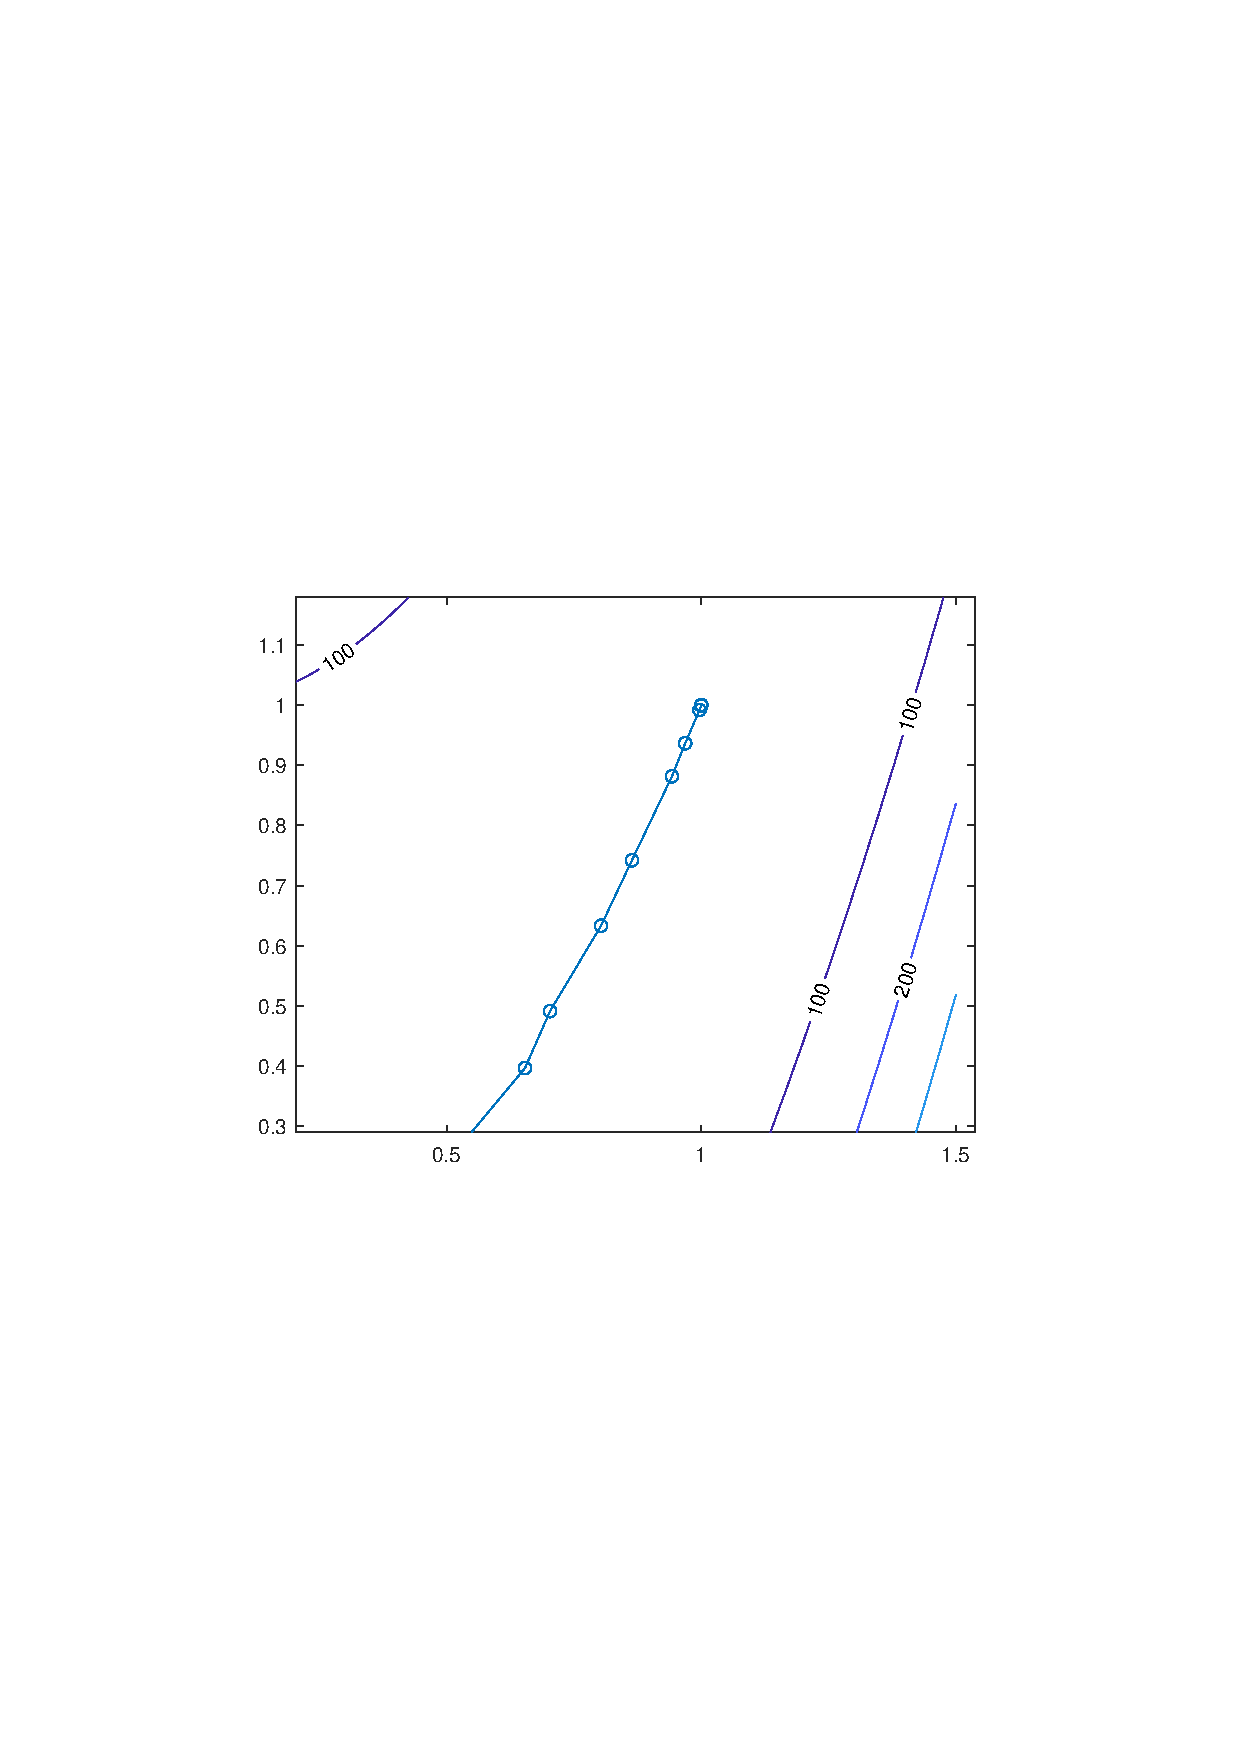
\includegraphics[width=5cm]{fig/4_42.pdf}}
\subfigure{
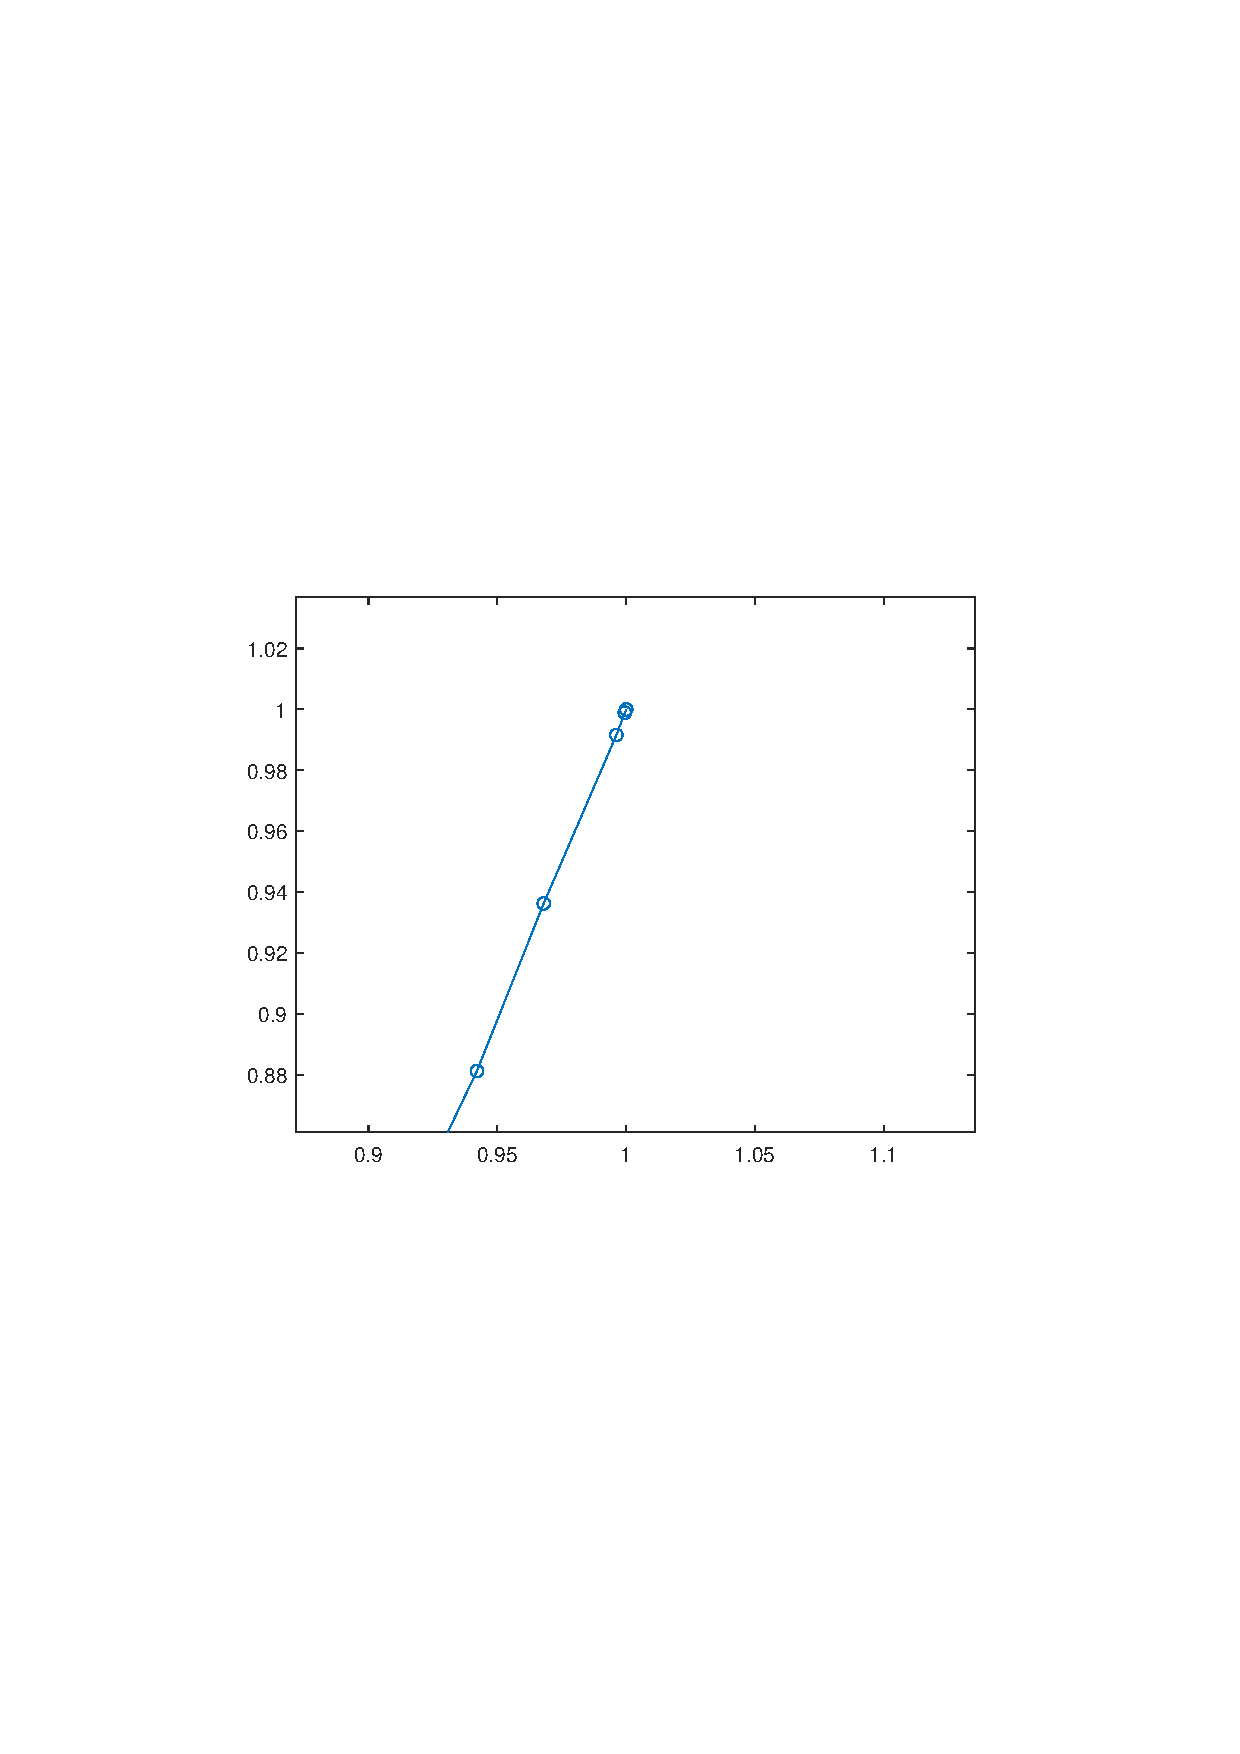
\includegraphics[width=5cm]{fig/4_43.pdf}}
\subfigure{
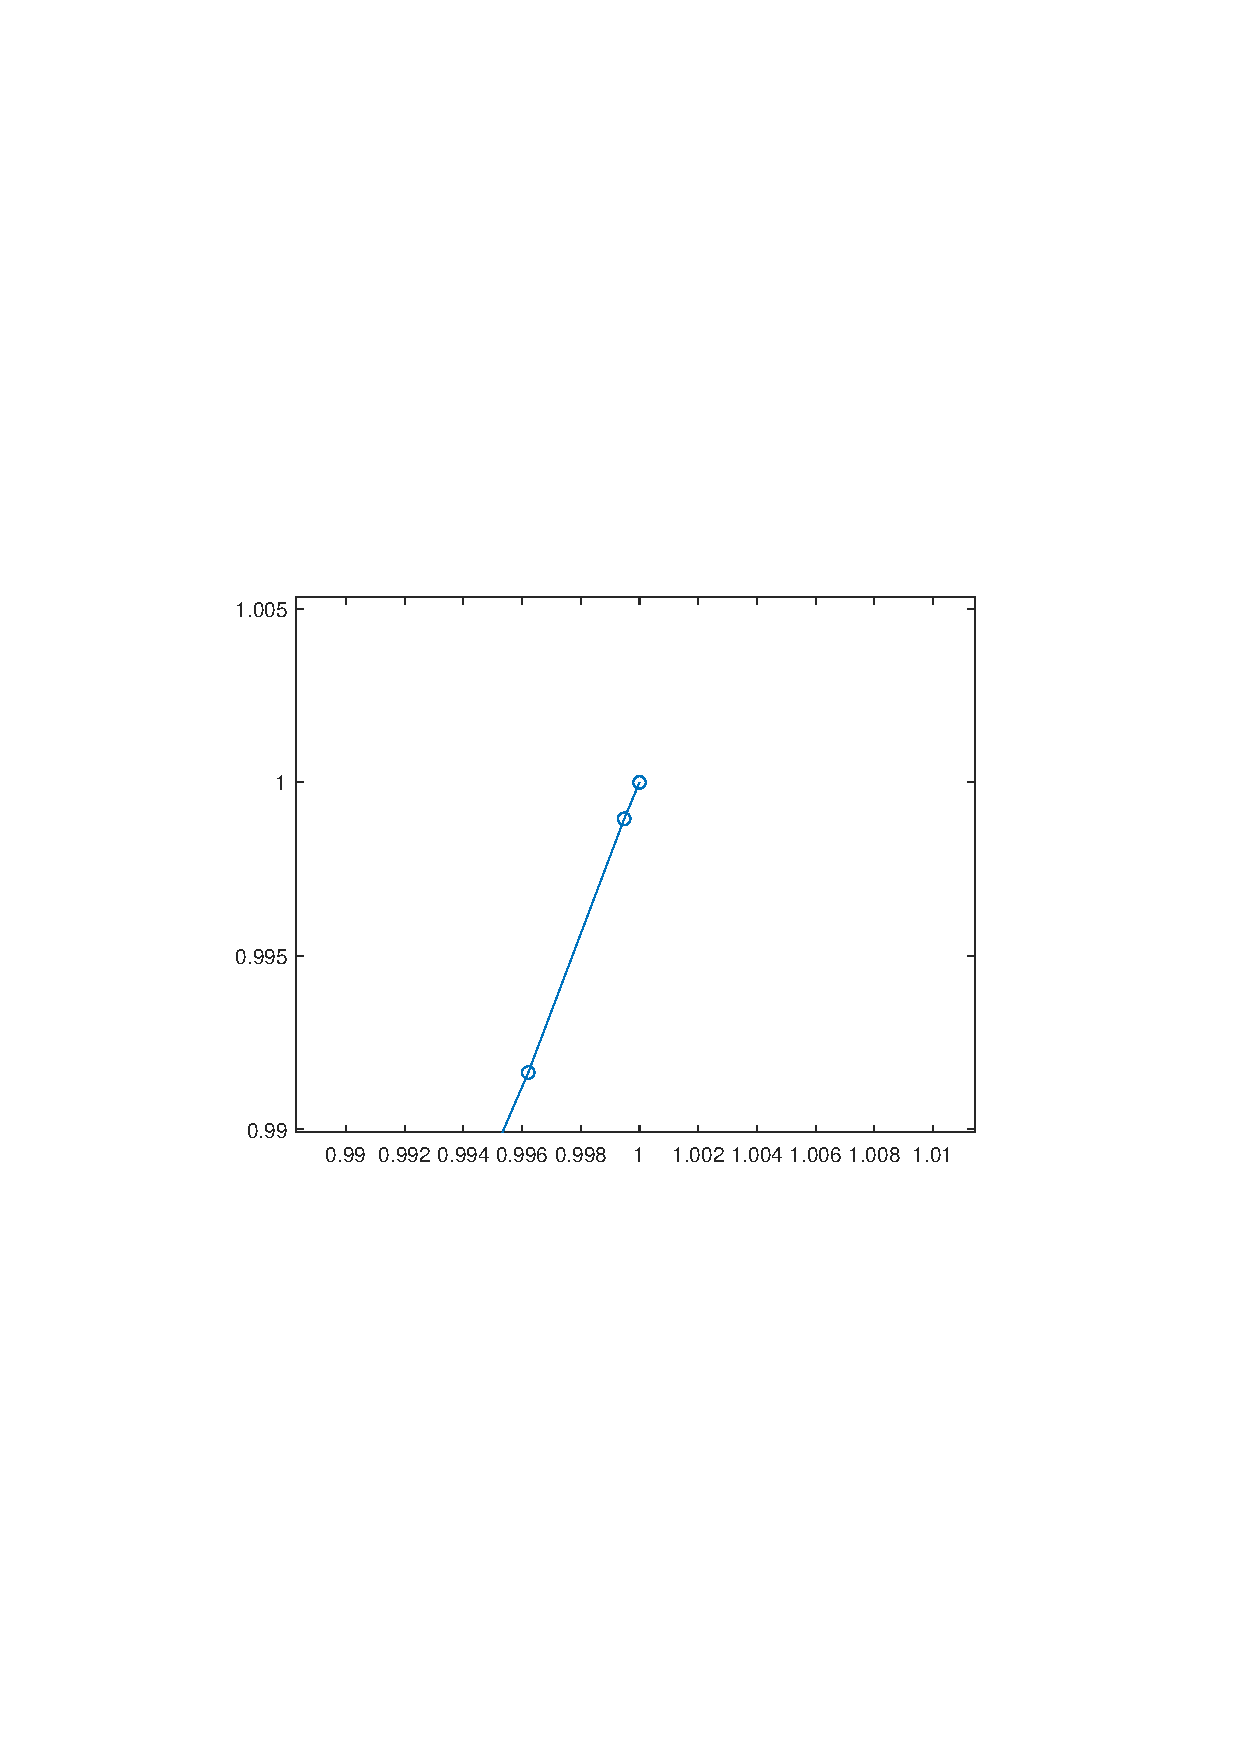
\includegraphics[width=5.3cm]{fig/4_44.pdf}}
\caption{Newton-Armijo in (-1.2,1)}
\label{Fig.lable}
\end{figure}

\begin{figure}[H]
\centering
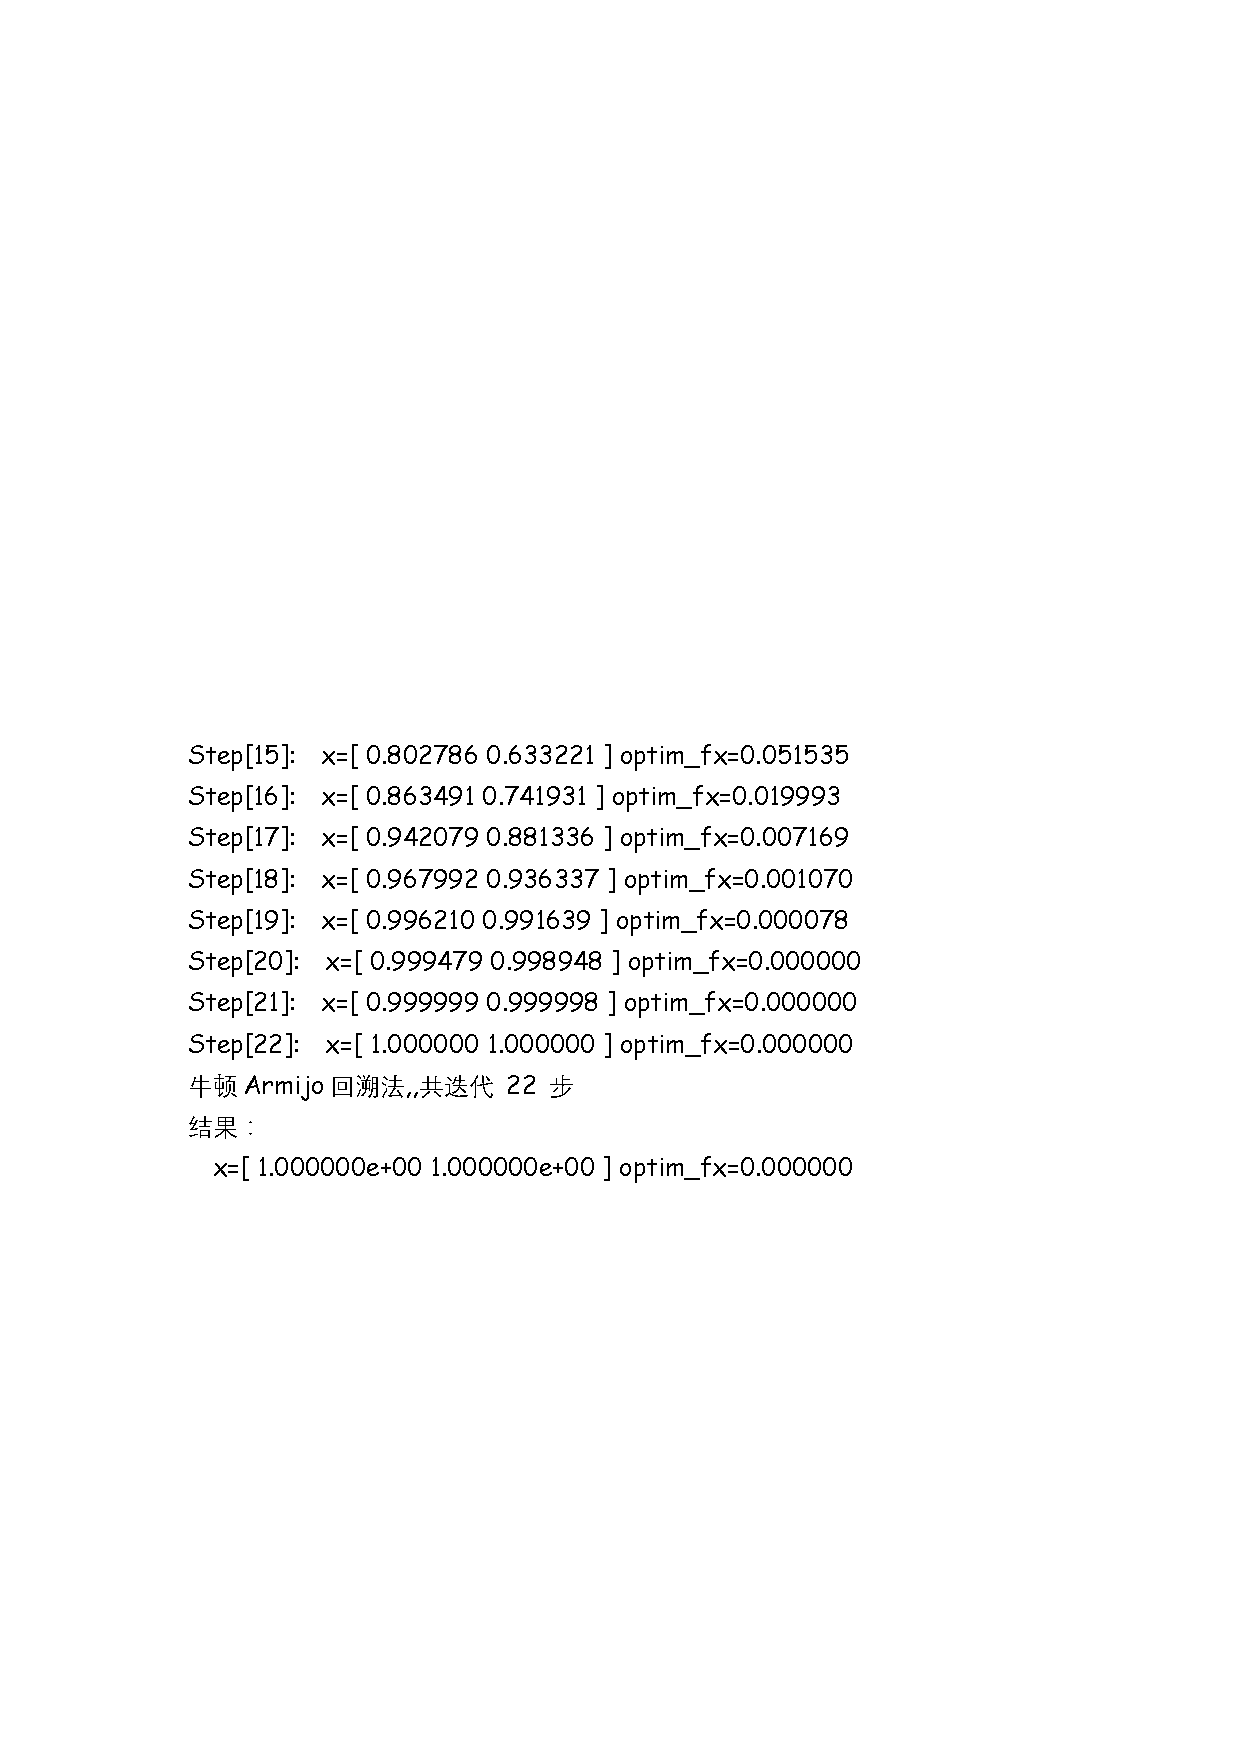
\includegraphics[width=10cm]{fig/4_45.pdf}
%\caption{在$(1,1)$处附近的三维等高线}
\end{figure}

\section{5.19}
迭代次数和求解的值如下:
\begin{table}[htbp]
  \centering
  \rowcolors{2}{blue!15}{blue!30}
    \begin{tabular}{cccc}
    \rowcolor{gray!50}
    \textbf{n=5} & \textbf{n=8} & \textbf{n=12} & \textbf{n=20} \\
    \rowcolor{lightgray!50}
    k=6   & k=19  & k=35  & k=66 \\
    \rowcolor{gray!50}
    x     & x     & x     & x \\
    5.00E+00 & 5.90E-11 & -9.61E+00 & -1.10E+01 \\
    -1.20E+02 & -6.97E-11 & 8.15E+02 & 1.05E+03 \\
    6.30E+02 & -5.16E-10 & -1.65E+04 & -2.40E+04 \\
    -1.12E+03 & 1.12E-09 & 1.36E+05 & 2.20E+05 \\
    6.30E+02 & 3.17E-10 & -5.36E+05 & -9.65E+05 \\
          & -6.55E-10 & 1.03E+06 & 1.99E+06 \\
          & -6.57E-10 & -6.43E+05 & -1.25E+06 \\
          & 4.59E-10 & -6.58E+05 & -1.34E+06 \\
          &       & 8.04E+05 & 8.83E+05 \\
          &       & 6.63E+05 & 1.69E+06 \\
          &       & -1.24E+06 & 3.88E+05 \\
          &       & 4.66E+05 & -1.31E+06 \\
          &       &       & -1.71E+06 \\
          &       &       & -5.28E+05 \\
          &       &       & 1.21E+06 \\
          &       &       & 2.00E+06 \\
          &       &       & 9.45E+05 \\
          &       &       & -1.43E+06 \\
          &       &       & -2.65E+06 \\
          &       &       & 1.89E+06 \\
    \end{tabular}%
  \label{tab:addlabel}%
\end{table}%

\section{5.27}
此题采用线搜索确定步长时,得到的结果误差极大,因为$\phi'(0)$在离稳定点较远时数量级高达$10^{40}$量级,导致线搜索得到的步长极小,几乎为0,无法收敛,经反复调整参数都没能取得好的结果,最后只好手动确定步长$\alpha_k=0.05$,此时效果良好,残量的2-范数随迭代次数的下降情况如下:(由于数量级巨大,为了更好的显示残差的波动,将原图中将残差取对数处理后并排参考)

\begin{figure}[H]
\centering
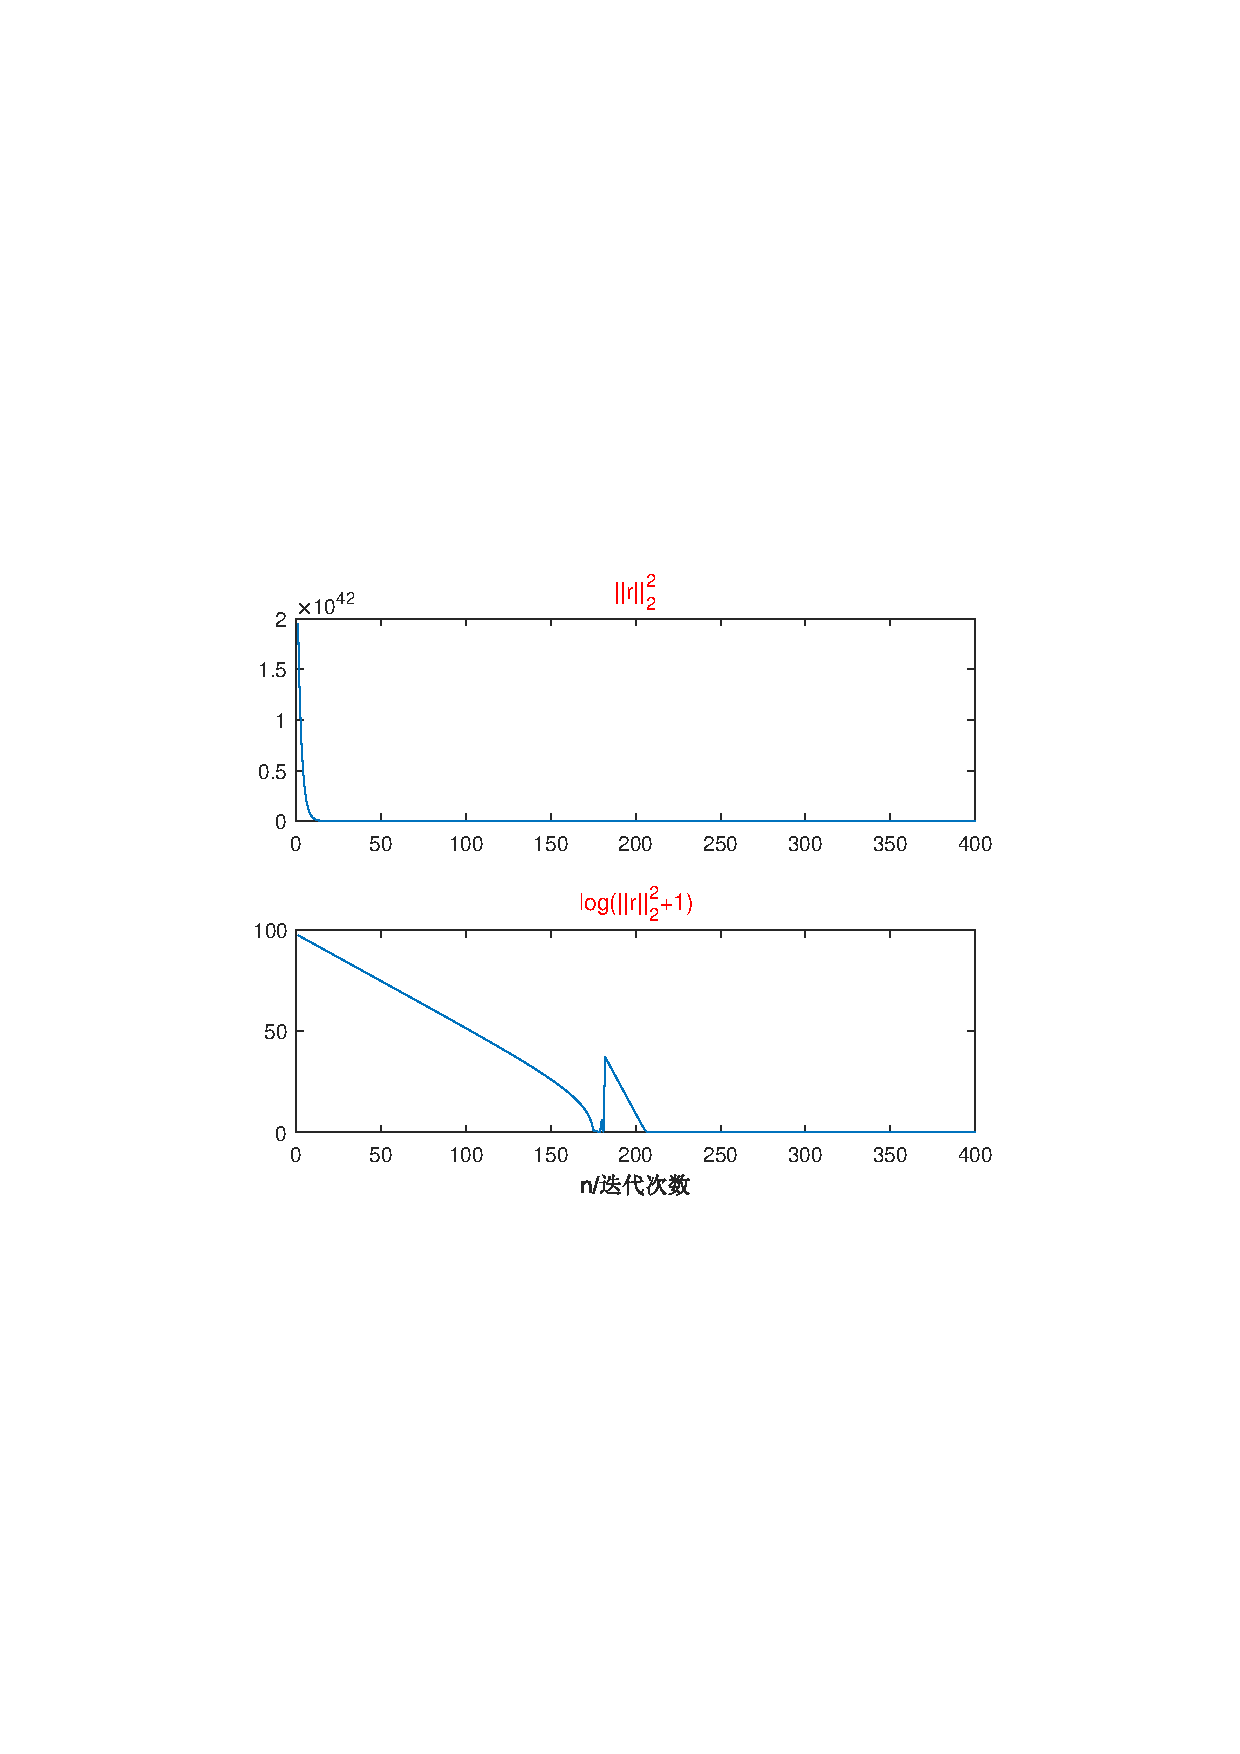
\includegraphics[width=12cm]{fig/6_1.pdf}
\end{figure}



又采用MATLAB中优化工具箱中的lsqnonlin函数进行拟合,得到的结果比我的程序算出来的略好,将两者进行比较,比较结果如下:

\begin{figure}[H]
\centering
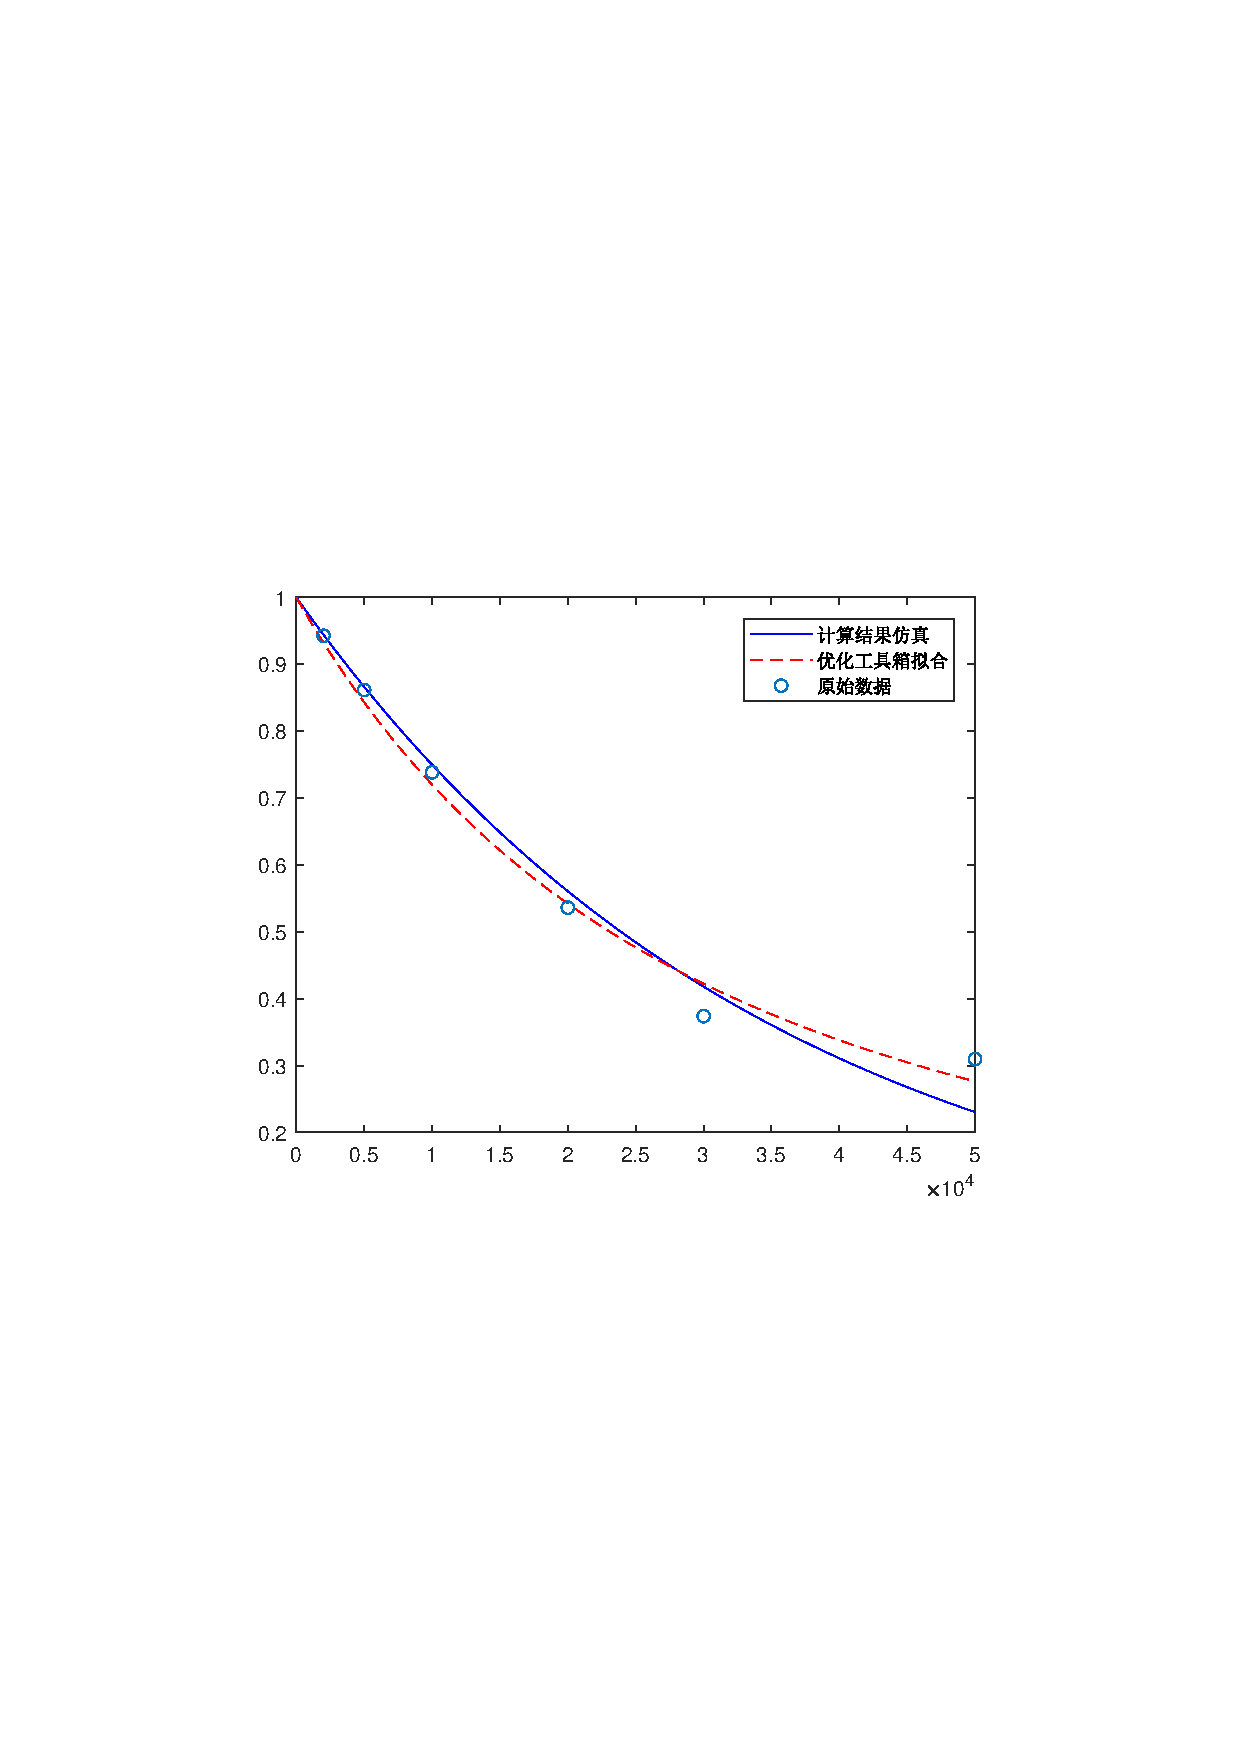
\includegraphics[width=12cm]{fig/6_2.pdf}
\end{figure}


\begin{table}[H]
\centering
\caption{结果比较}
	\begin{tabular}{ccc}
	\toprule
	{}&程序计算&工具箱拟合\\
	\midrule
	stv&0.125639950119876&0.104420208306470\\
	$x_1$&3.323336983976929e-04&-0.009615612533368\\
	$x_2$&3.516673367231929e+02&-19.446505801429495\\
	\bottomrule
	\end{tabular}
\end{table}



\end{document}